%%%%%%%%%%%%%%%%%%%%%%%%%%  phdsymp_sample2e.tex %%%%%%%%%%%%%%%%%%%%%%%%%%%%%%
%% changes for phdsymp.cls marked with !PN
%% except all occ. of phdsymp.sty changed phdsymp.cls
%%%%%%%%%%                                                       %%%%%%%%%%%%%
%%%%%%%%%%    More information: see the header of phdsymp.cls   %%%%%%%%%%%%%
%%%%%%%%%%                                                       %%%%%%%%%%%%%
%%%%%%%%%%%%%%%%%%%%%%%%%%%%%%%%%%%%%%%%%%%%%%%%%%%%%%%%%%%%%%%%%%%%%%%%%%%%%%%


%\documentclass[10pt]{phdsymp} %!PN
\documentclass[twocolumn]{phdsymp} %!PN
%\documentclass[12pt,draft]{phdsymp} %!PN
%\documentstyle[twocolumn]{phdsymp}
%\documentstyle[12pt,twoside,draft]{phdsymp}
%\documentstyle[9pt,twocolumn,technote,twoside]{phdsymp}

\usepackage[english]{babel}       % Voor nederlandstalige hyphenatie (woordsplitsing)

\usepackage{graphicx}			% Om figuren te verwerken.
\graphicspath{{../../../images/}}
\usepackage{booktabs}
\usepackage{times}
\usepackage{siunitx}
\usepackage{xcolor}
\usepackage{amsmath}
\PassOptionsToPackage{hyphens}{url}
\usepackage{hyperref}
\usepackage{url}

\usepackage[acronym,toc,shortcuts]{glossaries}
\setglossarystyle{super}
\renewcommand{\glsnamefont}[1]{\textbf{#1}}
\makeglossaries




%-------------------------------- acroniemen

\newacronym{UABS}{UABS}{Unmanned Arial Base Station}
\newacronym{EIRP}{EIRP}{equivalent isotropic radiation power}
\newacronym{UE}{UE}{User Equipment}
\newacronym{IEC}{IEC}{International Electrotechnical Commission}
\newacronym{SAR}{SAR}{Specific Absorption Rate}
\newacronym{whipp}{WHIPP}{WiCa Heuristic Indoor Propagation Prediction}
\newacronym{DL}{DL}{downlink}
\newacronym{UL}{UL}{uplink}
\newacronym{LTE}{LTE}{Long-Term Evolution}
\newacronym{FDD}{FDD}{Frequency Division Duplex}
\newacronym{TDD}{TDD}{Time Division Duplex}
\newacronym{ICNIRP}{ICNIRP}{International Commission on Non-Ionizing Radiation Protection}
\newacronym{LOS}{LOS}{line of sight}
\newacronym{NLOS}{NLOS}{non line of sight}
\newacronym{Exp Opt}{Exp. Opt.}{exposure optimized}
\newacronym{PwrC Opt}{PwrC. Opt.}{power consuption optimized}
\newacronym{WHO}{WHO}{World Health Organization}
\newacronym{FCC}{FCC}{Federal Communications Commission}
\newacronym{USA}{USA}{United States of America}
\newacronym{IOT}{IoT}{Internet of Things}
\newacronym{UAV}{UAV}{Unmanned Aerial Vehicle}
\newacronym{EU}{EU}{European Union}
%--------------------------------- woordenlijst
\newglossaryentry{isotropicradiator}{
	name = equivalent isotropic radiator,
	text = equivalent isotropic radiator,
	description = A theoretical source of electromagnetic waves which radiates the same intensity for all directions
}

\newglossaryentry{spuriousradiation}{
	name = spurious radiation,
	text = spurious radiation,
	description = According to the thefreedictionary.com: Any emission from a radio transmitter at frequencies outside its frequency band. Also known as spurious emission
}

\newglossaryentry{RRP}{
	name = RRP,
	text = RRP,
	description = RRP is an abreviation used in this paper to indicate an extension on EIRP and stands for Real Radiation Pattern. An RRP value indicates the power (in dBm) for a certain location unlike an EIRP where the power (in dBm) is independent of the location
}

\newglossaryentry{power flux density}{
	name = power flux density,
	text = power flux density,
	description = Magnitude of power ($W$) that travels through a curtain area ($m^2$)
}

\newglossaryentry{thermoregulatory capacity}{
	name = thermoregulatory capacity,
	text = thermoregulatory capacity,
	description = The capacity of an organism to regulate body temperture
}

%\printglossary[type=\acronymtype,title={Lijst van acroniemen}]
%\addcontentsline{toc}{chapter}{\textcolor{maincolor}{Lijst van acroniemen}}
%\printglossary
%\addcontentsline{toc}{chapter}{\textcolor{maincolor}{Verklarende woordenlijst}}






\hyphenation{si-mu-la-ted re-a-lis-tic packets really in-clu-ding}

\def\BibTeX{{\rm B\kern-.05em{\sc i\kern-.025em b}\kern-.08em
    T\kern-.1667em\lower.7ex\hbox{E}\kern-.125emX}}

\newtheorem{theorem}{Theorem}

\begin{document}

\title{	Evaluatie van de elektromagnetische blootstelling van de mens in een netwerk van drones}

\author{Thomas Detemmerman}

\supervisor{Wout Joseph, Luc Martens, Luc Martens, German Dario Castellanos Tache}

\maketitle

\begin{abstract}
De hedendaagse samenleving vertrouwt meer dan ooit op de aanwezigheid van draadloze netwerken. 
Tevens groeit ook de bezorgdheid bij de menigte over de elektromagnetische straling die hierbij gebruikt wordt. De overheid hanteert dan ook
strenge richtlijnen waaraan mobiele toestellen en zendmasten moeten voldoen.

Dit onderzoek tracht de specifieke absorptie snelheid van elektromagnetische straling in kaart te brengen door rekening te houden met alle mobiele 
toestellen en zendmasten. Om dit te verwezelijken wordt gebruik gemaakt van een tool ontwikkeld door de onderzoeksgroep WAVES aan de UGent. Deze tool
simmuleert een volledig netwerk waarbij zendmasten bevestigd worden aan drones. Dit onderzoek observeert verder hoe deze drones kunnen worden aangestuurd
zodoende dat bepaalde doelstellingen zoals het minimaliseren van energieverbruik of elektromagnetische straling bereikt kunnen worden.

Uit de resultaten blijkt dat...
\end{abstract}

\begin{keywords}
LTE, elektromagnetische blootstelling, energieverbruik, drone, femtocell, microstrip patch antenne, stralingspatroon, specifieke absorptietempo (SAT)
\end{keywords}

\section{Introductie}
\PARstart{D}{e} samenleving is meer dan ooit afhankelijk van draadloze communicatie.
Een elektronisch apparaat kan op elk gegeven moment in elke willekeurige plaats beroep doen 
op het draadloze netwerk, gaande van kleine \gls{IOT} apparatuur tot volwaardige zelf-rijdende auto's.

Ook in uitzonderlijke en mogelijks levensbedreigende situaties verwacht de samenleving de aanwezigheid 
van het mobiele netwerk. Desondanks het feit dat dit netwerk zelf mogelijks beschadigd is door de situatie.
Een mogelijk tijdelijke oplossing om een beschadigd network bij te staan is met behulp van onbemande vliegtuigen zoals drones.
Een base station kan geplaatst worden op een drone en zo effici\"ent verplaatst worden naar de nodige locatie.

Deze aanpak is niet alleen handig als het bestaande netwerk beschadigd is maar ook voor onverwachte toename aan gebruikers.
Bijvoorbeeld tijdens de aanslagen op de Brusselse Luchthaven zagen alle mobiele operatoren een toename in data verkeer.
Sommige operatoren raakten zodoende verzadigd dat ze als enige oplossing zagen om de wetgeving te negeren en de 
elektromagnetische straling te laten toenemen zodoende dat toch iedereen behandeld kon worden \cite{baseZaventem}.

De elektromagnetische straling die vrijkomt bij netwerken kunnen echter niet met onachtzaamheid behandeld worden.
Onderzoek toont aan dat buitensporige elektromagnetische straling verscheidinge biologische neveneffecten kunnen veroorzaken \cite{bioeffects,WHO}.
Het wordt dus duidelijk dat elektromagnetische straling een sleutelrol speelt bij het ontwikkelen van een met drones beholpen netwerk 
waarbij de wetgeving nauwkeurig nageleefd dient te worden.

Drone-gestuurde netwerken kunnen dankzij hun mobiliteit eenvoudig verplaatst worden. Verschillende onderzoeken 
tonen aan hoe deze netwerken geoptimaliseerd kunnen worden zodoende dat bepaalde doelstellingen zoals minimaal energieverbruik
bereikt kunnen worden.

Desondanks is er zeer beperkt onderzoek gedaan waarbij een drone-gestuurd netwerk wordt geoptimaliseerd naar elektromagnetische straling.
Verscheidene publicaties bespreken hoe elektromagnetische straling berekend kunnen worden maar 
overwegen zelden alle verschillende bronnen van straling.

Dit onderzoek stelt een methode voor waarbij rekening gehouden wordt met 
elektromagnetische straling en energieverbruik voor alle bronnen in een mobiel netwerk, zijnde: de gebruiker zijn eigen 
mobiel apparaat, de base station dat deze gebruiker aan het behandelen is, alle andere mobiele apparaten en 
alle andere base stations die andere gebruikers behandelen. Op deze manier kan duidelijk de bijdrage van elektromagnetische straling
 van elke bron duidelijk geïdentificeerd worden. 

Het gedrag van de elektromagnetische straling en het energieverbruik zullen geanalyseerd worden door de 
tool toe te passen op verschillende scenario's door gebruik te maken van verschillende soorten antennes, vlieghoogtes 
en bevolkingsdichtheden.
Waarden zoals \gls{SAR}, elektromagnetische straling en energieverbruik zullen inzicht 
geven in hoe het netwerk reageert op deze veranderede scenario's en hoe het netwerk 
ernaar te optimaliseren.

Om dit onderzoek mogelijk te maken zal een bestaande deployment tool, ontwikkeld
door de onderzoeksgroep WAVES van de universiteit van Ghent, uitgebreid worden. Deze tool 
beschrijft een volledig geconfigureerd drone netwerk wat een geschikt startpunt is voor dit onderzoek.

\section{State of the Art}
\subsection{Elektromagnetische Straling}

Personen in een mobiel network worden blootgesteld aan verscheidene bronnen van elektromagnetische straling, uitgedrukt in $V/m$.
Eenmaal deze elektromagnetische straling geabsorbeerd wordt door het menselijk lichaam spreken we van het specifieke absorptietempo (\gls{SAR}).
wat uitgedrukt wordt in $W/kg$. Al deze waarden zijn onderworpen aan limieten opgelegd door de overheid.
Dit onderzoek vindt plaats in Gent, een Vlaamse stad in Belgi\"e, waarbij voor het 2.6 GHz spectrum een individuele zendmast 
is gelimiteerd tot 4.5 V/m en de totale elektrische veldsterkte voor elk punt niet meer dan 31 V/m mag bedragen.  \cite{J23,S13_normenBelgie}. 
De maximale \gls{SAR} voor het volledige lichaam komende van een mobiel apparaat verspreid over een 
10 g tissue ($SAR_{10g}$) is beperkt tot $2 W/kg$ \cite{J30}. 

Verschillende onderzoeken berekenen de elektromagnetische veldsterkte van verschillende bronneen \cite{J6_originalExposureFormula,J1,J10_RDP,J10.1} 
waarbij sommigen de \gls{UL} elektromagnetische veldsterkte geconverteerd wordt naar locale \gls{SAR} \cite{J10_RDP,J10.1}. 
Met de naderende 5G technologie werd \cite{J17_kuehn2019modelling} gepubliceerd waarbij beschreven wordt hoe 
deze locale  \gls{SAR}-waarden van alle verschillende bronnen berekend kunnen worden en bij elkaar opgeteld worden.
Uiteindelijk beschrijft \cite{J22_plets2015joint} hoe de elektromagnetische veldsterkte omgezet kan worden 
naar \gls{SAR}-waarden voor het volledige lichaam.

In een realistisch netwerk kunnen sommige gebruikers telefoneren terwijl anderen andere vormen van telecommunicatie gebruiken zoals 
surfen op het internet. Aangezien de positie van het mobiel apparaat t.o.v. zijn gebruiker niet gekend is,
is het belangrijk dat de \gls{SAR}-waarden berekend worden in functie van het volledige lichaam. 

\subsection{Geoptimaliseerde drone-gestuurde netwerken}

Drones kennen verschillende toepassingen. Ze werden oorspronkelijk voornamelijk gebruikt door het leger waarbij ze dienst doen  
als camera bewaking of aanvallen zonder piloten in gevaar te brengen \cite{U12}. 
Deze drones zijn de laatste jaren in prijs gedaald waardoor ze beter toegankelijk worden
voor het algemene publiek. Hierdoor is het onderzoek naar nieuwe toepassingen ervan sterk toegenomen.

Een drone uitgerust met een femtocell base station wordt een \gls{UABS} genoemd en 
geniet verschillende voordelen zoals mobiliteit en snelle inzetbaarheid.
Desondanks zijn er ook verschillende nadelen zoals het beperkte gewicht dat een drone kan dragen 
en de schaarse energievoorziening.

Kawamoto et al. introduceert in \cite{U11} een WiFi netwerk  met behulp van drones waarbij rekending gehouden wordt
met de richting van de geplaatste antenes op de drone. 
Gangula et al. illustreert in \cite{U10} hoe drones gebruikt kunnen worden voor \gls{LTE}
en
Zeng et al. presenteerd in  \cite{U12} een handleiding waarbij uitdagingen   zoals energieverbruik, mobiliteit en 
de richting van de antenne voor een 5G netwerk besproken worden. 
In \cite{J2}, Deruyck et al. ontwikkeld een deployment tool voor een drone gestuurd netwerk voor rampsituaties waarbij 
een ideale vlieghoogte van 100 meter aangeraden wordt.  
Dit word verder uitgebreid in \cite{U1} waarbij ook rekening gehouden wordt met 
 direct-link backhaul connecties waarbij een ietwat lagere vlieghoogte van 80 meter bekomen wordt.

Mozaffari et al. voorziet in \cite{U3} richtlijnen hoe een een drone-gestuurd netwerk geoptimaliseerd en geanalyseerd kan worden.
Eén onderzoekggebied dat uitgebreid onderzocht wordt is het optimaliseren van de lacaties ware drones zich moeten bevinden.
Deze algoritmen trachten bepaalde doelstellingen zoals minimaal energieverbruik of kortste vlieg afstand te bereiken \cite{U6,U7,U8,U9}.
Deze optimalistatie kan gebeuren door verschillende implementaties waaronder exacte algoritmen of machinaal leren \cite{U3,U5}.

Onderzoek waarbij de elektromagnetische straling gelimiteerd wordt is echter beperkt.
Deruyck et al. bespreekt in \cite{J1} hoe een conventioneel mobiel netwerk geoptimaliseerd kan worden zodoende dat het energieverbruik 
van het volledige netwerk minimaal wordt of de elektromagnetische bloodstelling van een individu.
Echter onderzoek waarbij een drone-gestuurd netwerk geoptimaliseerd wordt naar elektromagnetische straling is 
door de auteur niet gekend.

\subsection{Technologies}
Voor het ontwikkelen van het netwerk zullen de meer robuuste drones van \cite{J2} gebruikt worden (details in tabel \ref{table:defaultconf}). De 
gekoppelde antennes zullen opereren in het 2.6 GHz spectrum. Aangezien het aangenomen wordt dat de gebruikers een voortdurende bloodstelling
van  elektromagnetische straling ondervinden zonder onderbrekingen, wordt frequency division duplexing gebruikt. 

% problem antennae on drones
De antenne op de drone zullen dienst doen als gateway tussen de mobiele apparaten op de grond en het backbone netwerk.
Bepalen welke antenne gebruikt moet worden en hoe deze vervolgens het beste gepositioneerd kan worden brengt 
verschillende uitdagingen met zich mee. Het stralingspatroon van de antenne kan be\"invloed worden door de drone \cite{A1}.
Maar ook het feit dat deze drones boven de gebruikers zullen vliegen zorgt er voor dat 2D modellering onvoldoende is.
Een 3D model waarbij rekening gehouden wordt met zowel horizontale als verticale richting zal een veresite vormen \cite{U12}.

Het eenvoudigste stralingspatroon is een hypothetische isotrope antenne dewelke straalt met gelijke hoeveelheid in elke richting.
Een antenne die gelijkwaardig straalt over een specifiek vlak wordt een omnidirectionele antenne genoemd 
\cite{U12}. Hiervan bestaan verschillende soorten zoals monopoolantennes, dipoolantennes en vleugel antennes \cite{A4,A10,A11,A12}.
Een andere vorm van antennes zijn directionele antennes dewelke energie besparen door de elektromagnetische straling daar 
te focussen waar het nodig is. Eén soort hiervan dat uitgebreid onderzocht  zijn in verscheidene antenne-arrays 
zijn de microstrip-antennes \cite{A5,A6,A8}.
Deze voorzien verschillende voordelen ten opzichte van meer traditionele antennes 
\cite{J13_microstripadvantages,J14_antennadesign} zoals het beperkte gewicht, lage productiekosten en aerodynamica.

Een microstrip-antennes is opgebouwd uit een grondplaat en een stralingsplaat met daartussen een di\"electrisch substraat.
Verscheidene variates bestaan zoals microstrip patch antennes, microstrip slot antennes and geprinte dipool antennes. 
dewelke allemaal gelijkende karakteristieken hebben \cite{J13_microstripadvantages,J14_antennadesign}. 
Ze zijn allemaal dun, ondersteunen dubbele frequenties and hebben allemaal het nadeel dat 
ze interferentie kunnen veroorzaken op frequenties buiten het bedoelde spectrum. 
De microstrip patch en slot antenne ondersteunen beide circulaire en lineaire pollarisatie terwijl de geprinte dipool antenne enkel 
lineare polarisatie ondersteund. Verder is de microstrip patch antenne het eenvoudigste te produceren ten opzichte 
van de andere overwogen antennes \cite{J13_microstripadvantages}. 

Figuur \ref{fig:exampleDrone} toont een microstrip patch antenne dewelke bestaat 
uit aluminium die bevestigd is op een substraat van teflon. De microstrip patch antenna 
wijst naar de grond aangezien de drone boven de mensen zal vliegen.

\begin{figure}[h]
\centering
  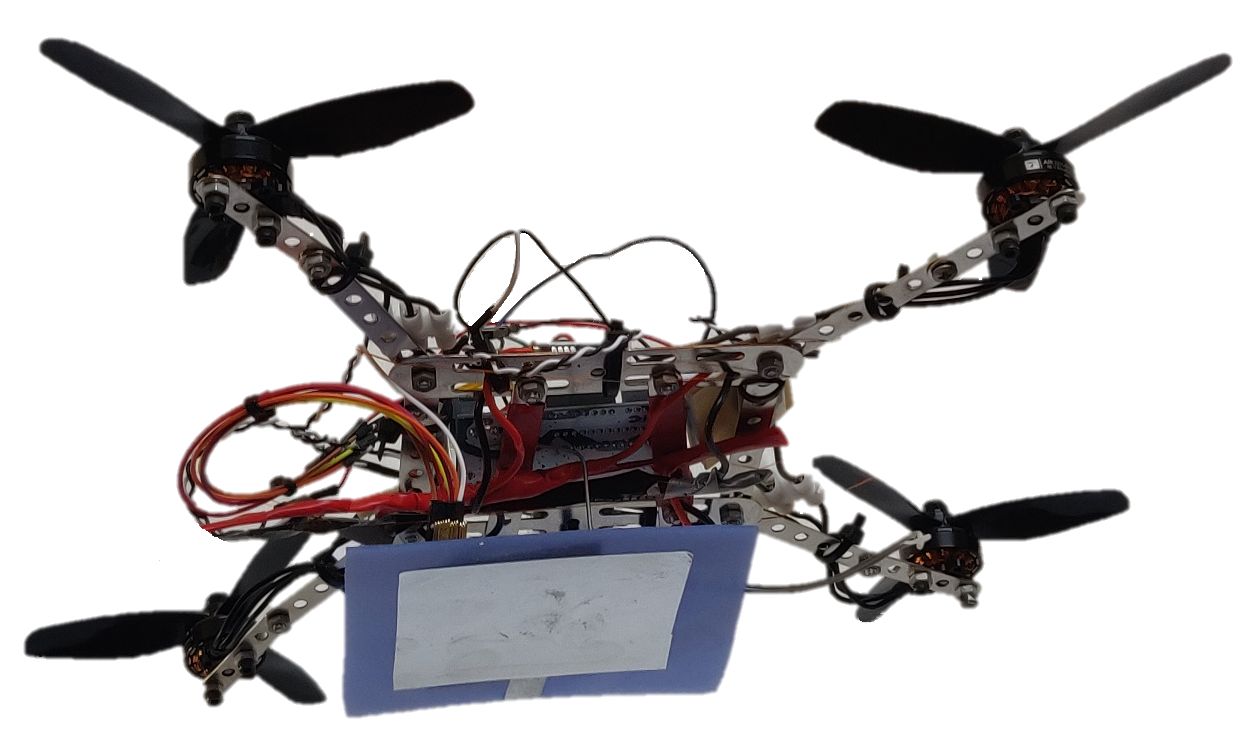
\includegraphics[width=\linewidth]{drone.png}
  \caption{Image of a microstrip patch antenna attached to the bottom of a \gls{UAV}. }
  \label{fig:exampleDrone}
\end{figure}

\section{Methodologie}
\subsection{Elektromagnetische Straling}
\subsubsection{Totale Electromagnetische Straling}
De totale \gls{SAR} voor het volledige lichaam ($SAR^{wb,total}_{10g}$) van een individu 
can berekend worden als een eenvoudige som van de \gls{SAR}-waarden van de verschillende bronnen. 
Dit is gebaseerd op de formule in \cite{J17_kuehn2019modelling} dewelke aanneemt dat het mobiele apparaat 
tegen het oor van zijn gebruiker gehouden wordt. Hierdoor worden alle waarden in locale \gls{SAR}-waarden voor het hoofd uitgedrukt.
In dit netwerk is de plaats van het mobiele apparaat echter  niet  gekend wat zou leiden tot incorrecte conclusies. Bijgevolg 
zal alles uitgedrukt worden in functie van het volledige lichaam.

\begin{equation} 
\begin{aligned}
SAT^{wb,total}_{10g} = SAT^{wb,myUE}_{10g} +  SAT^{wb,myUABS}_{10g} \\
+ SAT^{wb,otherUE}_{10g} + SAT^{wb,otherUABSs}_{10g}
\end{aligned}
\label{eq:overallSARwb}
\end{equation}

In bovenstaande formule staat $wb$ voor whole body oftewel het volledige lichaam en $UE$ voor User Equipment oftewel het mobiele apparaat op de grond.
De eerste parameter, $SAT^{wb,myUE}_{10g}$, duidt de geabsorbeerde elektromagnetische straling aan komende van de gebruik zijn eigen apparaat.
Ondanks het feit dat de \gls{UL} straling bedoeld is voor het \gls{UABS} die deze gebruiker behandeld,
een deel van deze straling wordt ook geabsorbeerd door zijn gebruiker. 
Dit komt vanwege het omnidirectionele gedrag van de gsm zijn antenne.
Een tweede parameter is $SAT^{wb,myUABS}_{10g}$ dewelke de straling aanduid veroorzaakt door \gls{DL} dataverkeer, komende van de \gls{UABS} die deze gebruiker behandeld.
Als derde parameter hebben we $SAT^{wb,otherUE}_{10g}$ dewelke de straling aanduidt veroorzaakt door andere gebruikers hun mobiel apparaat.
Als laatste stelt $SAT^{wb,otherUABSs}_{10g}$ de \gls{DL} straling voor komende van alle \gls{UABS}en die andere gebruikers behandelen.
Een illustratie is te vinden in \ref{fig:networkIllustration} waarbij de groene pijl straling in het nabije veld voorstellen en alle andere 
pijlen straling in het verre veld voorstellen.

\begin{figure}[h!]
\centering
  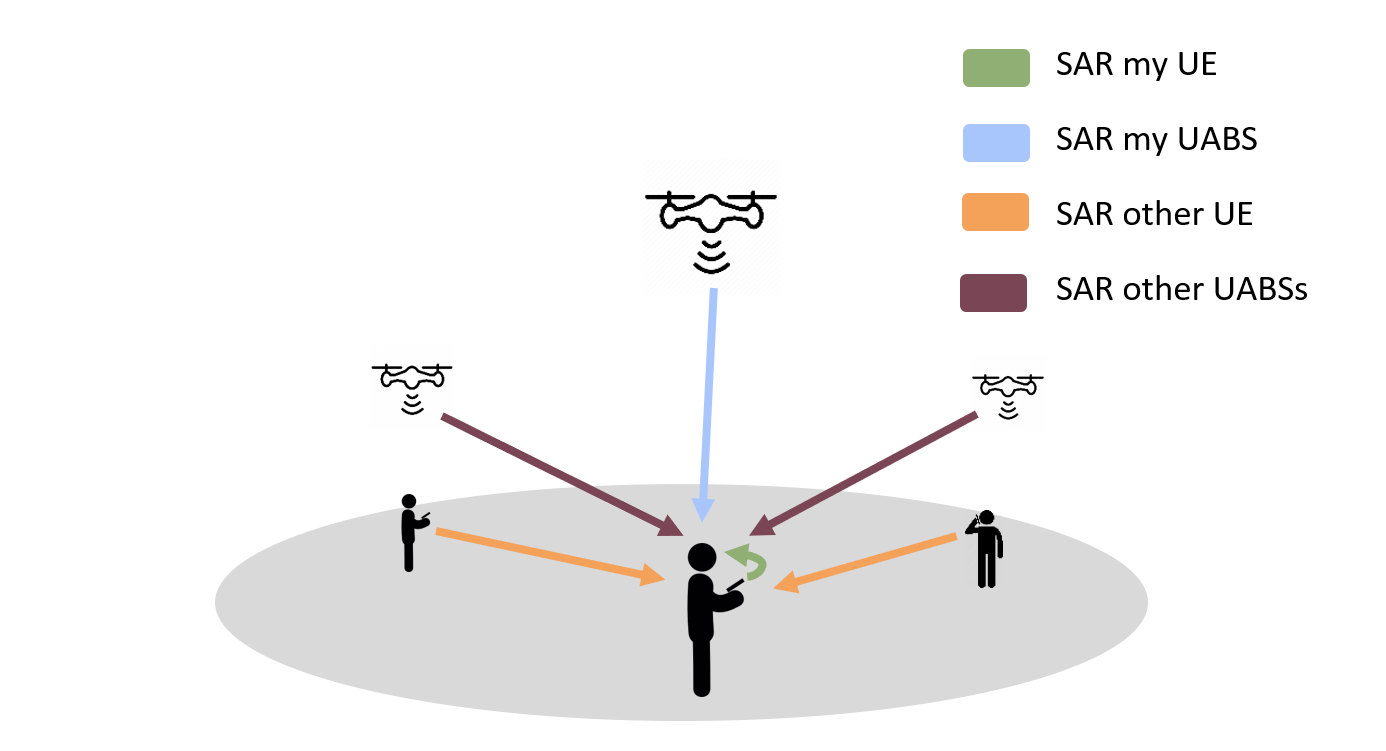
\includegraphics[width=\linewidth]{networkIllustrationSARSources.png}
  \caption{Deze illustratie toont hoe de gemiddelde gebruiker (hier getoond in het midden) be\"invloed worden door verschillende bronnen van elektromagnetische straling.}
  \label{fig:networkIllustration}
\end{figure}

\subsubsection{Electromagnetische straling van een indivuele bron}
\label{sec:calculatingexposure}

De elektromagnetische veldsterkte berekenen in een bepaald punt in het verre veld wordt gedaan worden voor alle \gls{UABS}'en en 
alle mobiele apparaten behalve het apparaat in dat punt. Dit zal namelijk straling in het nabije veld zijn en dient anders berekend te worden. 
De elektromagnetische veldsterkte $E$ voor het individu $u$ komende van een brom $i$ wordt als volgt berekend.

\begin{equation}
E_i(u) [V/m] = 10^{\frac{ES(u)[dBm] - 43.15 + 20*\log(f [MHz])- PL(u) [dB]}{20}}
\label{eq:singleexposure}
\end{equation}

Het berekenen van de effectieve straling (ES) voor een gebruiker $u$ vereist eerst om de  \gls{EIRP}-waarde te hebben berekend 
 \cite{J6_originalExposureFormula,J1}. Dit kan bekomen worden door de zendvermogen $P_t$ op te tellen met de zendversterking $G_t$
 en het aftrekken van het kabelverlies $L_t$.
 Deze formule dient echter uitgebreid te worden zodoende dat er rekening gehouden wordt met signaalverzwakking die komt met
 verschillende stralingspatronen. Deze waarde hangt af van de hoek tussen de gebruiken en de richting waarnaar de antenne wijst. 
 De signaalverzwakking bij een \gls{isotropicradiator} is altijd nul ongeacht de hoek.
 Dit leidt tot de volgende formule.

\begin{equation}
\begin{aligned}
RRP [dBm] = P_t [dBm] + G_t [dBi]- L_t [dB]\\
     - attenuation(u) [dB]
\end{aligned}
\label{eq:eirp}
\end{equation}

De gebruikte frequentie $f$ in formule \ref{eq:singleexposure} is uitgedrukt in MHz. Aangezien 
\gls{LTE} gebruikt wordt zal deze waarde 2600 MHz bevatten.

Als laatste dient formule \ref{eq:singleexposure} ook het padverlies $PL$ te kennen.
Een geschikt propagatie model dient gekozen te worden. Hier wordt geopteerd voor het 
Walfish-Ikegami model aangezien deze goed presteerd voor femtocell netwerken in stedelijke gebieden \cite{J2}.

\subsubsection{Samenvoegen van meerdere bronnen}

De totale elektromagnetische straling $E_{tot}$ in een bepaald punt, komende van alle verschillende bronnen kan berekend worden 
m.b.v. formule \ref{eq:totalexposure}. Hierin staat $E_i$ voor de elektromagnetische veldsterkte voor dat punt komende van bron $i$
en $n$ staat voor alle bronnen in het verre veld van een bepaalde categorie wat hier ofwel \gls{UABS}'s of mobiele apparaten van andere personen.
$E_{tot}$ zal berekend worden in elk punt waar er zich een gebruiker bevindt.
\begin{equation}
E_{tot} [V/m] = \sqrt{\sum_{i=1}^{n} (E_i [V/m]) ^2}
\label{eq:totalexposure}
\end{equation}

\subsubsection{Omzetten van elektromagnetische veldsterkrte naar \gls{SAR}}

Formule \ref{eq:overallSARwb}  verwacht dat de \gls{SAR} waarden in functie van het volledige lichaam uitgedrukt zijn.
Om de elektromagnetische veldsterkte te kunnen omzetten daar deze \gls{SAR}-waarden dient er een onderscheid gemaakt te worden 
tussen bronnen in het nabije veld ($SAR^{wb,nf}$) en het verre veld ($SAR^{wb,ff}$).
$SAR^{wb,myUABS}_{10g}$ is een bron waarbij de gebruiker zich in het nabije veld bevindt terwijl 
de gebruiker zich voor alle andere bronnen in het verre veld bevindt.

Het omzetten van deze waarden gebeurd door middel van een conversie constante dewelke gebaseerd is op 
Duke van de Virtual Family. Duke is een 34 jarige man met een gewicht van 72 kg, een hoogte van 1.74 en 
een bmi van 23.1 kg/m \cite{J22_plets2015joint}. 
Onderzoek toont aan dat conversie constante voor WiFi in het verre veld $0.0028 \frac{W/kg}{W/m^2}$ bedraagt
en  0.0070 $\frac{W/kg}{W}$ in het nabije veld \cite{J22_plets2015joint}.
WiFi maakt gebruik van het 2400 MHz spectrum wat heel dichtbij \gls{LTE} valt (2600 MHz). Daarom 
wordt in \cite{J22_plets2015joint} aangenomen dat de conversie  constante ook van toepassing is voor \gls{LTE}.

Het berekenen van \gls{SAR} in het verre veld  word bijgevolg als volgt gedaan.

\begin{equation}
S [W/m^2]= \frac{(E_{tot} [V/m])^2}{337}
\label{eq:flux}
\end{equation}
\begin{equation}
SAR^{wb,ff}_{10g} [W/kg]= S [W/m^2]* 0.0028 \left[\frac{W/kg}{W/m^2}\right]
\label{eq:DLconversion}
\end{equation}

De constante is vergelijking \ref{eq:DLconversion} zet de \gls{power flux density} $S$ om  naar de verwachtte $SAR^{ff,wb}_{10g}$.
Om dit mogelijk te maken moet 
de uitkomst van formule \ref{eq:totalexposure} eerst nog omgezet worden naar \gls{power flux density} met behulp van formule
\ref{eq:flux}.

De \gls{SAR} die veroorzaakt wordt door het mobiel apparaat in het nabije veld kan gevonden worden door 
het zendvermogen $P_{tx}$ van het  apparaat te vermenigvuldigen met de conversie constante voor het nabije veld.
\begin{equation} 
SAR^{wb,nf}_{10g} \left[\frac{W}{kg}\right] = 0.0070 \left[\frac{W/kg}{W}\right] * P_{tx} [W]
\label{eq:ulToSar}
\end{equation}

De energie die door het mobiele aparaat wordt gebruikt kan berekend worden met formule \ref{eq:powerUE} \cite{J22_plets2015joint}.
\begin{multline} 
P_{tx}^{UE} = min \big\{P_{max} [dBm] , \\
 P_{pusch} [dBm] + \alpha * PL [dB] + 10log(M) + \sigma \big\}
\label{eq:powerUE}
\end{multline}

\subsection{Microstrip Patch Antenne}
Een microstrip patch antenne is gekozen vanwege zijn eenvoudige productieproces maar voornamelijk vanwege het
 lage gewicht en aerodynamica wat heel voordelig is wanneer het aan een drone gekoppeld wordt \cite{J13_microstripadvantages}.

De dimensies van de antenne hangen af van de gebruikte frequentie en de eigenschappen van het di\"electrisch substraat.
De antenne zal opereren met een frequentie $f_0$ van 2.6 GHz. 
Elk substraat heeft een di\"electrische constante $\epsilon_r$ dat de doorlaatbaarheid 
van eht substraat aanduid en hangt af van het gebruikte materiaal.
Substraten met een hoge di\"electrische constante en kleine hoogte zullen de dimensies van de antenne reduceren 
terwijl  een lager di\"electrische constante met een hogere hoogte de performantie van de 
antenne zullen bevorderen \cite{J14_antennadesign,J15_antennadesign}. 
Voor dit onderzoek is glas het gekozen substraat vanwege zijn hogere di\"electrische constante
van $\epsilon_r = 4.4$ ten opzichte van andere materialen zoals Teflon met een di\"electrische constante
van $\epsilon_r = 2.2$ \cite{J14_antennadesign}. 
Glass met een hoogte van 2.87 mm 
zal de dimensies van het volledige antenne opperlakte verminderen wat 
voordelig is bij de beperkte ruimte die beschikbaar is op een drone.

\begin{table}[h!]
\centering
\begin{tabular}{|l|c|l|}
\hline
 beschrijving            & symbool          & waarde         \\    \hline
 middenfrequentie      & $f_0$           & 2600 Hz       \\ 
 di\"electrische constante    & $\epsilon_r$    & 4.4         \\ 
 Hoogte van het substraat & $h$             & 0.00287 m    \\ \hline
\end{tabular}
\caption{Overzicht van de configuratie parameters}
\label{table:antennaparas}
\end{table}

De dimensies van de stralingsplaat kunnen berekend worden met de formules uit \cite{J14_antennadesign,J15_antennadesign}.
Dit leidt tot een stralingsplaat van 35.09 mm bij 26.55 mm en  een grondplaat van minstens 52.40 mm bij 43.80 mm.
De resulterende microstrip patch antenne is ge\"illustreerd in figuur \ref{fig:basicpatchantenna} en zal resulteren 
in het stralingspatroon getekend in figuur \ref{fig:radpattern}.
\begin{figure}[h!]
\centering
  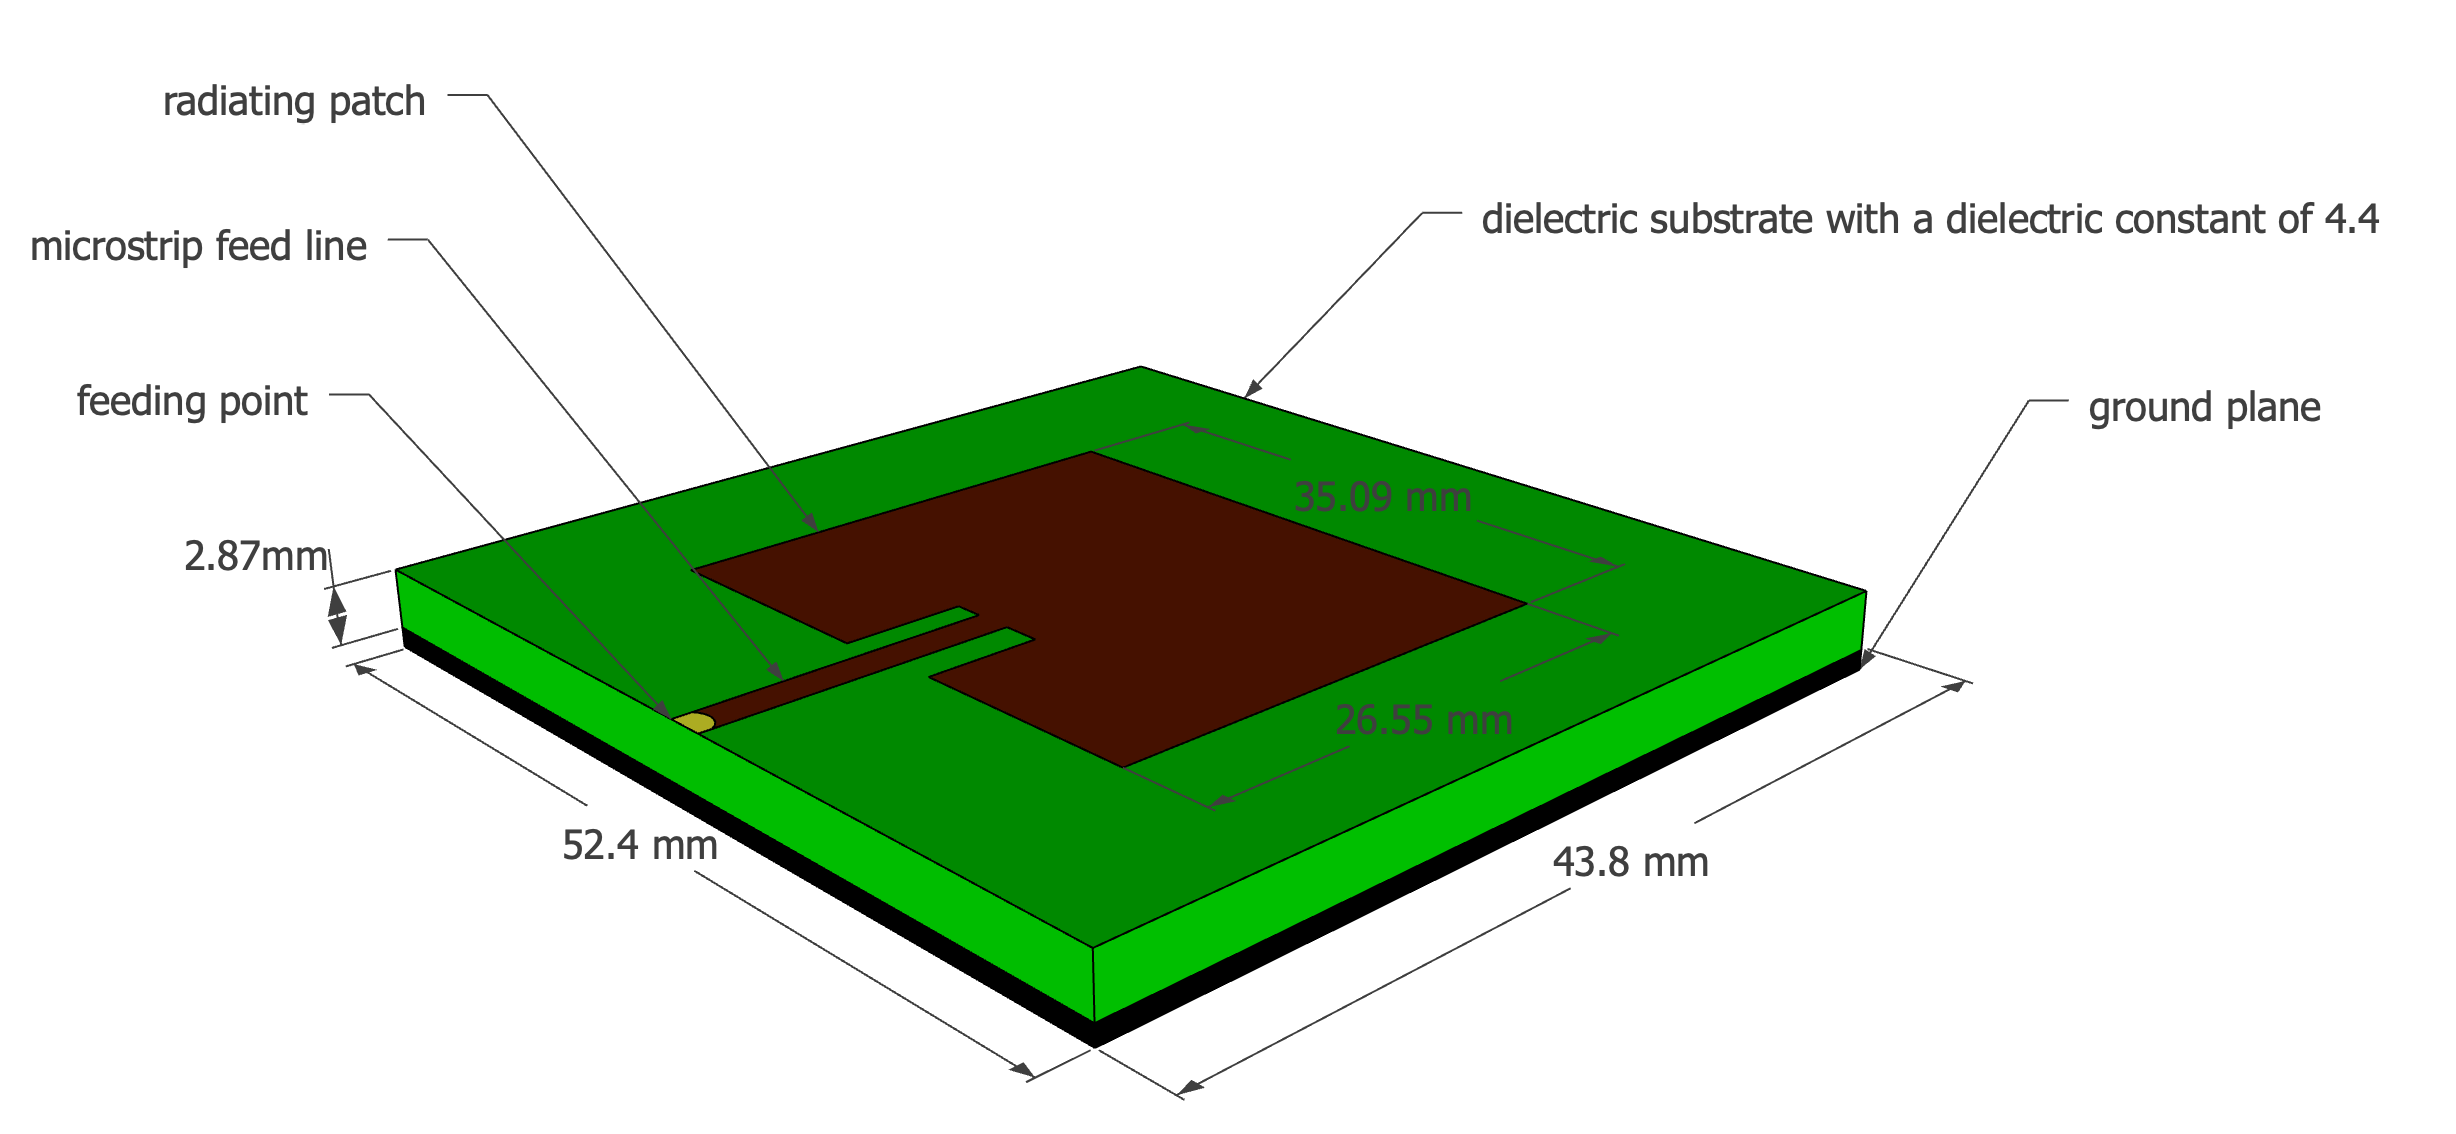
\includegraphics[width=\linewidth]{MicrostripAntenna.png}
  \caption{Design van een microstrip patch antenne.}
  \label{fig:basicpatchantenna}
\end{figure}


\begin{figure}[!htb]
\minipage{0.50\linewidth}
  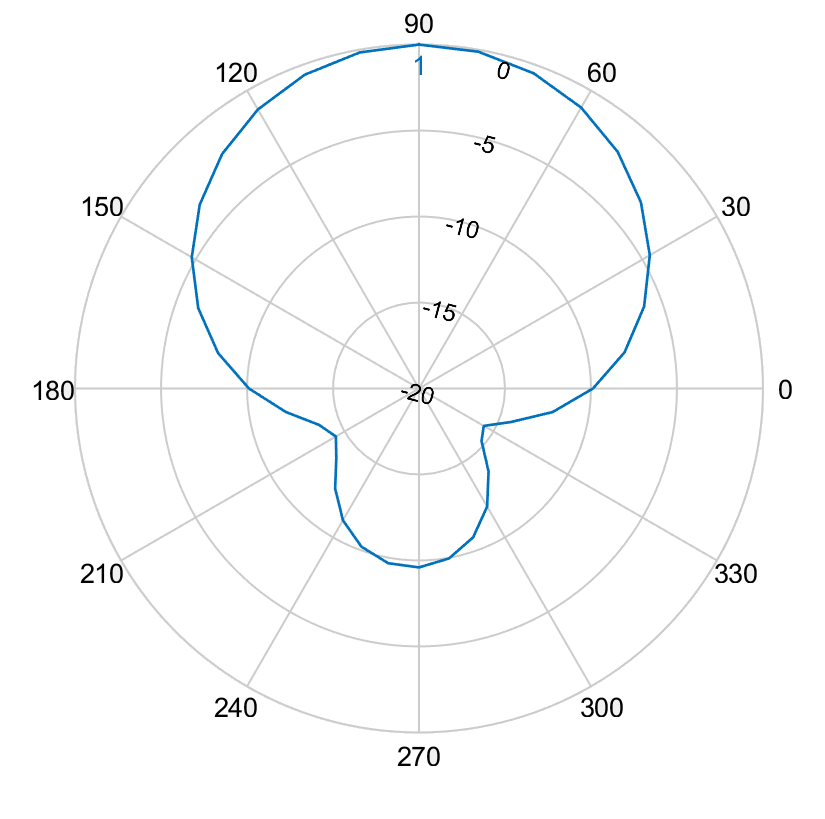
\includegraphics[width=\linewidth]{pattern2/ep.png} 
\endminipage\hfill
\minipage{0.50\linewidth}%
  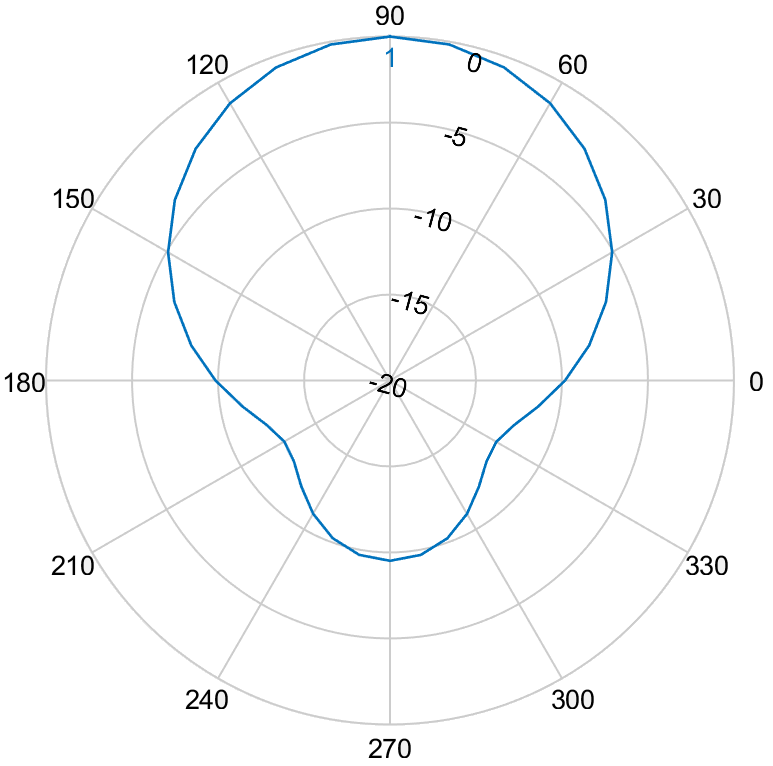
\includegraphics[width=\linewidth]{pattern2/hp.png}
\endminipage
  \caption{Links is het stralingspatroon voor het E-vlak en rechts voor het H-vlak.}
\label{fig:radpattern}
\end{figure}

\subsection{Optimaliseren van het netwerk}

Deruyck et al. bespreekt in \cite{J1} hoe een traditioneel mobiel netwerk geoptimaliseerd kan worden naar
Hoewel een toenemend zendvermogen wel degelijk resulteert in een toenemend elektromagnetische veldsterkte is deze regel niet van 
toepassing indien we het energieverbruik bekijken over het hele netwerk heen. 
De auteurs van \cite{J1} tonen een omgekeerd equivalente relatie aan.
De reden hierachter is dat het vaak goedkoper is op gebied van energie om de elektromagnetische straling van een al actieve base station 
verder te laten toenemen i.p.v.  een nieuwe base station te activeren. Dit leidt tot de volgende fitness functie dewelke
gebaseerd is op \cite{J1}.

\begin{equation} 
f = w * \left(1 - \frac{E_m}{E_{max}}\right) + (1 - w)*\left(1 - \frac{P}{P_{max}}\right) * 100
\label{eq:fitnessfunction}
\end{equation}

Formule \ref{eq:fitnessfunction} geeft een gewicht terug dat aanduid hoe goed het netwerk preseteerd.
$w$ is de belangrijkheidsfactor die loopt van 0 tot 1, grenzen inbegrepen. Een $w$ gelijk aan 0 betekend
dat elektromagnetische straling niet belangrijk is. Een dergelijk network wordt een \gls{PwrC Opt} netwerk genoemd.
Aan de andere kant, een $w$ gelijk aan 1 impliceert dat het minimaliseren van elektromagnetische bloodstelling top prioriteit is
en zal bijgevolg resulteren in een \gls{Exp Opt} netwerk. $P_{max}$ is het energieverbruik van alle \gls{UABS}'s op maximaal 
zendvermogen, ongeacht of ze 
op non-actief staan of niet.
$P$ representeerd de effectieve verbruikte energie van het huidig ontwikkelde netwerk.
$E_m$ is de gewogen elektromagnetische straling van de gemiddelde gebruiken van het huidig ontwikkelde netwerk en 
$E_{max}$ is dezelfde waarde maar met alle \gls{UABS}'s op maximaal zendvermogen.

Bij het optimaliseren van het netwerk is het niet enkel belangrijk om  de gemiddelde gebruiker te overwegen maar ook het limiteren 
van extrema \cite{J1}. 
Daarom wordt er gebruik gemaakt van het gewogen gemiddelde waarbij niet enkel rekening gehouden wordt met de mediaan maar ook 
met het 95\textsuperscript{ste} percentiel. Dit leidt tot formule \ref{eq:em} waarbij 
  $w_1$ en  $w_2$ de gewichten zijn van respectievelijk de mediaan en 95\textsuperscript{ste} percentiel.
 Aangezien verondersteld wordt dat beiden waarden een gelijkwaardige rol spelen zullen beiden een gewicht van 0.5 krijgen. 

\begin{equation} 
E_m = \frac{w_1 * E_{50} + w_2 * E_{95}}{w_1 + w_2}
\label{eq:em}
\end{equation}

\begin{figure}[h!]
  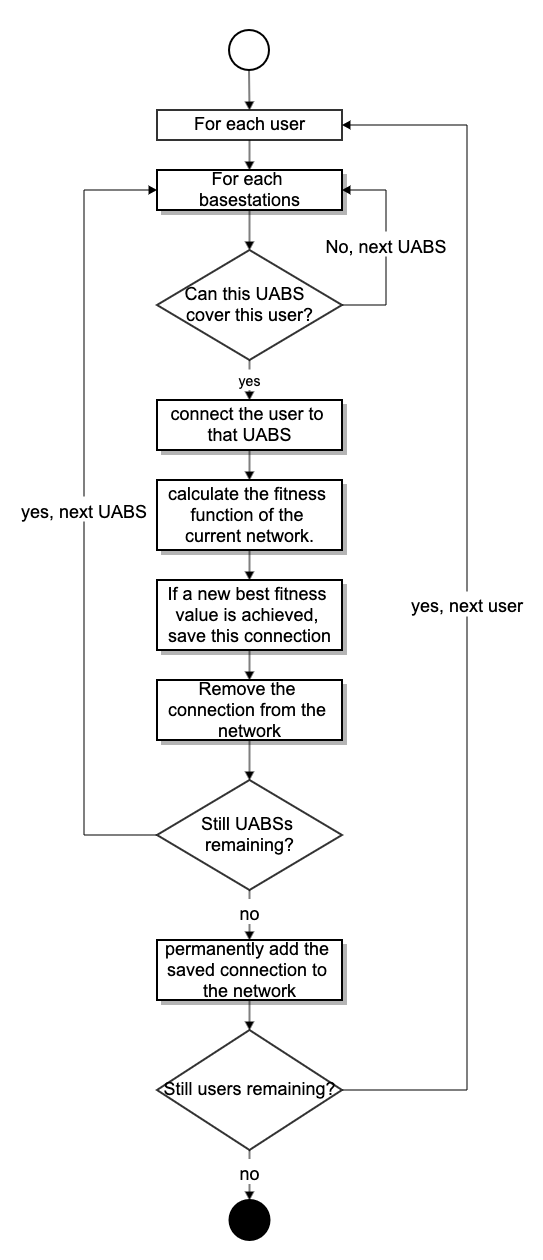
\includegraphics[height=0.8\textheight]{decisionAlgoFlowChart.png}
  \caption{Flowchart of the decision algorithm.}
  \label{fig:decisionAlgoFlowChart}
\end{figure}

\subsection{Simulatie Tool}

\subsubsection{Hoofdalgoritme}
In eerste instantie dient een beschrijving van het gebied voorzien te worden. Dit wordt verwezenlijkt met behulp van 
zogenaamde shape-bestanden. Deze bestanden bevatten een volledige beschrijving van de vorm van elk gebouw. Vervolgens 
worden gebruikers uniform verdeeld over het gebied en zal er een tijdelijke \gls{UABS} geplaatst worden boven elke gebruiker?
Nu is het aan het beslissingsalgoritme om te bepalen welke \gls{UABS}s effectief zal blijven en hoe hoog het zendvermogen van elke \gls{UABS}
zal zijn. Eens het beslissingsalgoritme voltooid is zal de tool controleren of het nummer van online drones niet meer is dat 
de capaciteit van de stockageruimte toelaat. Indien dit wel het geval is zullen drones offline gehaald worden, beginnend bij 
drones die het minste personen behandelen.

\subsubsection{Beslissingsalgoritme}

Het oplossen van het netwerk wordt gedaan door het beslissingsalgoritme en start met het berekenen van het padverlies tussen 
alle gebruikers en tussen gebruikers en drones. Hierna doorloopt het algoritme elke gebruiker waarbij getracht wordt deze te verbinden 
met elke mogelijke drone. Deze verbinding is niet altijd mogelijk omdat een drone al reeds verzadigd kan zijn met andere gebruikers of 
de drone is zo ver verwijderd van deze gebruiker dat het de maximale toegestane zendvermogen zou overschreiden.
Indien een verbinding toch mogelijk is zal de gebruiker met deze drone verbonden worden en zal een score toegekend worden met behulp van 
de fitness functie  \ref{eq:fitnessfunction}. 
Dit proces wordt herhaald voor elke drone. Uitsluitend de verbinding dat resulteert in de beste score voor het volledige netwerk 
zal gebruikt worden. Wanneer de laatste gebruiker behandeld is geweest, bekomen we een volledig netwerk voor een ongelimiteerd aantal drones.
Het network wordt vervolgens terug aan het hoofdalgoritme gegeven voor eventueel verdere afhandeling.
Een stroomdiagram van dit algoritme is gegeven in figuur \ref{fig:decisionAlgoFlowChart}.

%%%%%%%%%%%%%%%%%%%%%%%%%%%%%%%%%%%%%%%%%%%%%%%%%%%%%%%%%%%%%%%%%%%%%%%%%%%%%%%%%%%%%%%%%%%%%%%%%%%%%%%%%%%%%%%%%%%

\section{Scenario's}

De standaard configuratie is gegeven in tabel \ref{table:defaultconf} en is altijd van toepassing tenzij anders vermeld.
\begin{table}[!htb]
\centering
\begin{tabular}[t]{ll}
        \toprule
        \multicolumn{2}{l}{\textbf{Mobiel netwerk}} \\
        \hline
        \hspace{3mm}  technologie        & LTE     \\
        \hspace{3mm}  frequentie         & 2.6 GHz \\
        \hspace{3mm}  Power offset ($P_{pusch}$)            & -120 dBm  \\
        \hspace{3mm}  Compenstatie voor padverlies ($\alpha$)   & 1  \\
        \hspace{3mm}  Correctie waarde                    & 0 dBm  \\
        \hspace{3mm}  Aantal resource blokken      & 100  \\
        \hline
        \multicolumn{2}{l}{\textbf{Drone}} \\
        \hline  
        \hspace{3mm}  energie drone        & 13.0 A   \\
        \hspace{3mm}  gemiddelde snelheid        & 12.0 m/s \\
        \hspace{3mm}  gemiddeld energieverbruik      & 17.33 Ah    \\
        \hspace{3mm}  voltage batterij       & 22.2 V \\
        \hline
        \multicolumn{2}{l}{\textbf{Femtocell antenna}} \\
        \hline  
        \hspace{3mm}  maximum $P_{tx}$          & 33 dBm   \\
        \hspace{3mm}  richting van de antenne   & neerwaards   \\ 
        \hspace{3mm}  zendversterking           & 4 dBm   \\ 
        \hspace{3mm}  kabelverlies               & 2 dBm   \\ 
        \hspace{3mm}  implementation loss       & 0 dBm   \\
        \hspace{3mm}  stralingspatroon         & EIRP or\\
         \hspace{3mm}                           & microstrip patch\\
        \hspace{3mm}  vlieghoogte                & 100m  \\
        \hline
        \multicolumn{2}{l}{\textbf{UE Antenna}} \\
        \hline 
        \hspace{3mm} hoogte                     & 1.5m vanaf de vloer      \\ 
        \hspace{3mm} zendversterking                      & 0 dBm   \\ 
        \hspace{3mm} kabelverlies              & 0 dBm   \\ 
        \hspace{3mm} stralingspatroon         & EIRP  \\
        \hspace{3mm} aantal aanwezig in het netwerk         & 224  \\
        \toprule
\end{tabular}
\caption{Overzicht van de waarden voor een standaard configuratie.}
\label{table:defaultconf}
\end{table}

Drie scenario's zullen onderzocht worden. Het eerste zal \'e\'en enkele gebruiker en 
 \'e\'en enkele drone overwegen 
voor het gehele netwerk. De \gls{SAR}, elektromagnetische straling, energieverbruik  en 
het nodige zendvermogen van de antenne zullen onderzocht worden voor verschillende vlieghoogtes.

Bij het tweede scenario zal het netwerk uitgebreid worden met meerdere gebruikers maar 
er zal nog steeds uitsluitend  \'e\'en drone aanwezig zijn. De eerste onderzochte parameter 
is een varierende vlieghoogte gaande van 20 meter tot 200 meter. Hierbij zullen 224 gebruikers 
uniform verdeerld worden over het centrum van Gent. Dit is de gemiddelde populatiegroote op 
een werkdag om 17 uur in Gent \cite{J2}.
De tweede parameter is een varierende population lopend van 50 tot 600 gebruikers. Hierbij 
zal de vlieghooghte vastgezet worden op 100 meter \cite{J2}.
Het energieverbruik, electromagnetische straling en \gls{SAR} zullen onderzocht worden 
voor elke parameter.

Een derde scenario is sterk gelijkend aan het vorige. Dezelfde twee parameters zullen onderzocht 
worden maar nu voor een onbeperkt aantal \gls{UABS}s.

Vier configuraties zijn mogelijk voor elke onderzochte parameter in elk scenario.
Er zijn twee antenes overwogen, namelijk een \gls{isotropicradiator} en een microstrip patch antenne.
Beide kunnen opereren in een \gls{PwrC Opt} netwerk en een \gls{Exp Opt} netwerk. Dit maakt een totaal van 4 configuraties.
Een overzicht is gegeven in figuur \ref{fig:fourCasesMatrix}

Het is belangrijk om op te merken dat alle meetwaarden strikt gelimiteerd zijn tot de hiervoor vermoende bronnen en 
bijgevolg enkel dataverkeer overwegen tussen de gebruiker zijn gsm en de \gls{UABS}. 
Andere bronnen zoals connecties naar het backhaul network zullen niet overwogen worden.

\begin{figure}[h!]
  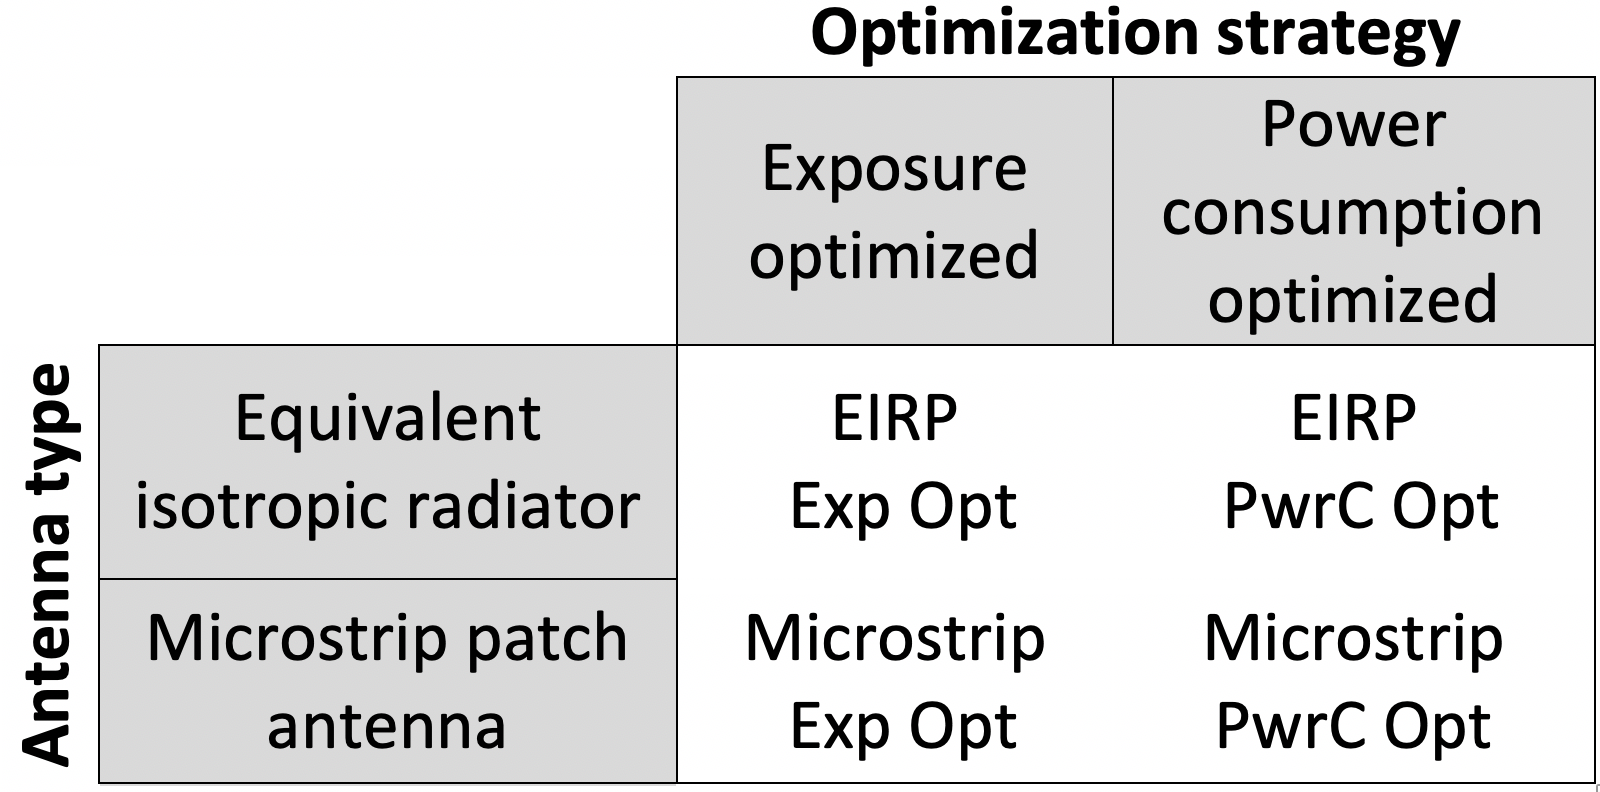
\includegraphics[width=\linewidth]{fourCasesMatrix.png}
  \caption{Matrix met de vier mogelijke configuraties.}
  \label{fig:fourCasesMatrix}
\end{figure}

\section{Results}
Vier configuraties zullen overwogen worden tijdens het evaluaren van twee parameters, zijnde 
populatie groote en vlieg hoogte. Deze parameters zullen onderzocht worden in drie scenarios 
door het gedrag van het energieverbruik, electromagnetische straling en \gls{SAR}-waarden te monitoren.
De electromagnetische straling en \gls{SAR} zullen genonmen worden van de gewogen gemiddelde gebruiker
m.b.v. vergelijking \ref{eq:em} waarbij $w_{1}$ en $w_{2}$ gelijk gesteld zijn aan 50\%. 
Elk resultaat wordt uitgemiddeld over 20 simmulaties.


\subsection{E\'en gebruik en \'e\'en \gls{UABS}}
De resultaten tonen dat voor een variabele vlieghoogte, een logaritmische relatie bestaat tussen de 
 $P_{tx}$ en de vlieghooghte.
 Dit komt door de logaritmische schaal waarin de decibels van de $P_{tx}$ zijn in uitgedrukt.
Elke keer rdat de vlieghoogte te hoog wordt neemt de $P_{tx}$ met \'e\'en dBm toe.
Voor een stanaard configurartie met een maximum $P_{tx}$ van 33 dBm en een \gls{LOS} verbinding kan een 
\gls{UABS} tot 387 m hooghte vliegen voor het verliezen van de connectie.

Dit scenario is onderzocht voor een microstrip patch antenne die energieverbruik minimaliseerd.
De gekozen optimalisatie maakt echter niet uit aangezien er uitsluitend \'e\'en \gls{UABS} beschikbaar is.
Het beslissing's algoritme bepaalt welke gebruiker met welke \gls{UABS} verbonden wordt.
Aangezien er maar een \gls{UABS} beschikbaar is is zullen beide optimalisatie technieken gelijkaardig werken.
Verder zal de gebruikte antenne ook geen verschil maken. 
De gebruiker zal zich namelijk boor beide antennes in de hoofdbeam van het stralingspatroon 
bevinden waar in beide gevallen geen verzwakking van het signaal is.




Tijdens het onderzoeken van verschillende vlieghoogte's stellen de resultaten vast  dat
\gls{UL} straling exponentieel toeneemt terwijl de \gls{DL} straling constant blijft op 
10 $nW/kg$. De reden dat de \gls{DL} straling constant blijft is vanwege power control dat ervoor zorgt
dat niet meer energie gebruikt wordt dan strikt noodzakelijk. 
Daardoor kan bevestigd worden dat de elektromagnetische straling een constante fractie is van energie en afstand.
De \gls{UL} straling start laag met 1 $nW/kg$ maar steekt de \gls{DL} straling voorbij rond de 80 meter.

\begin{figure}[]
\centering
  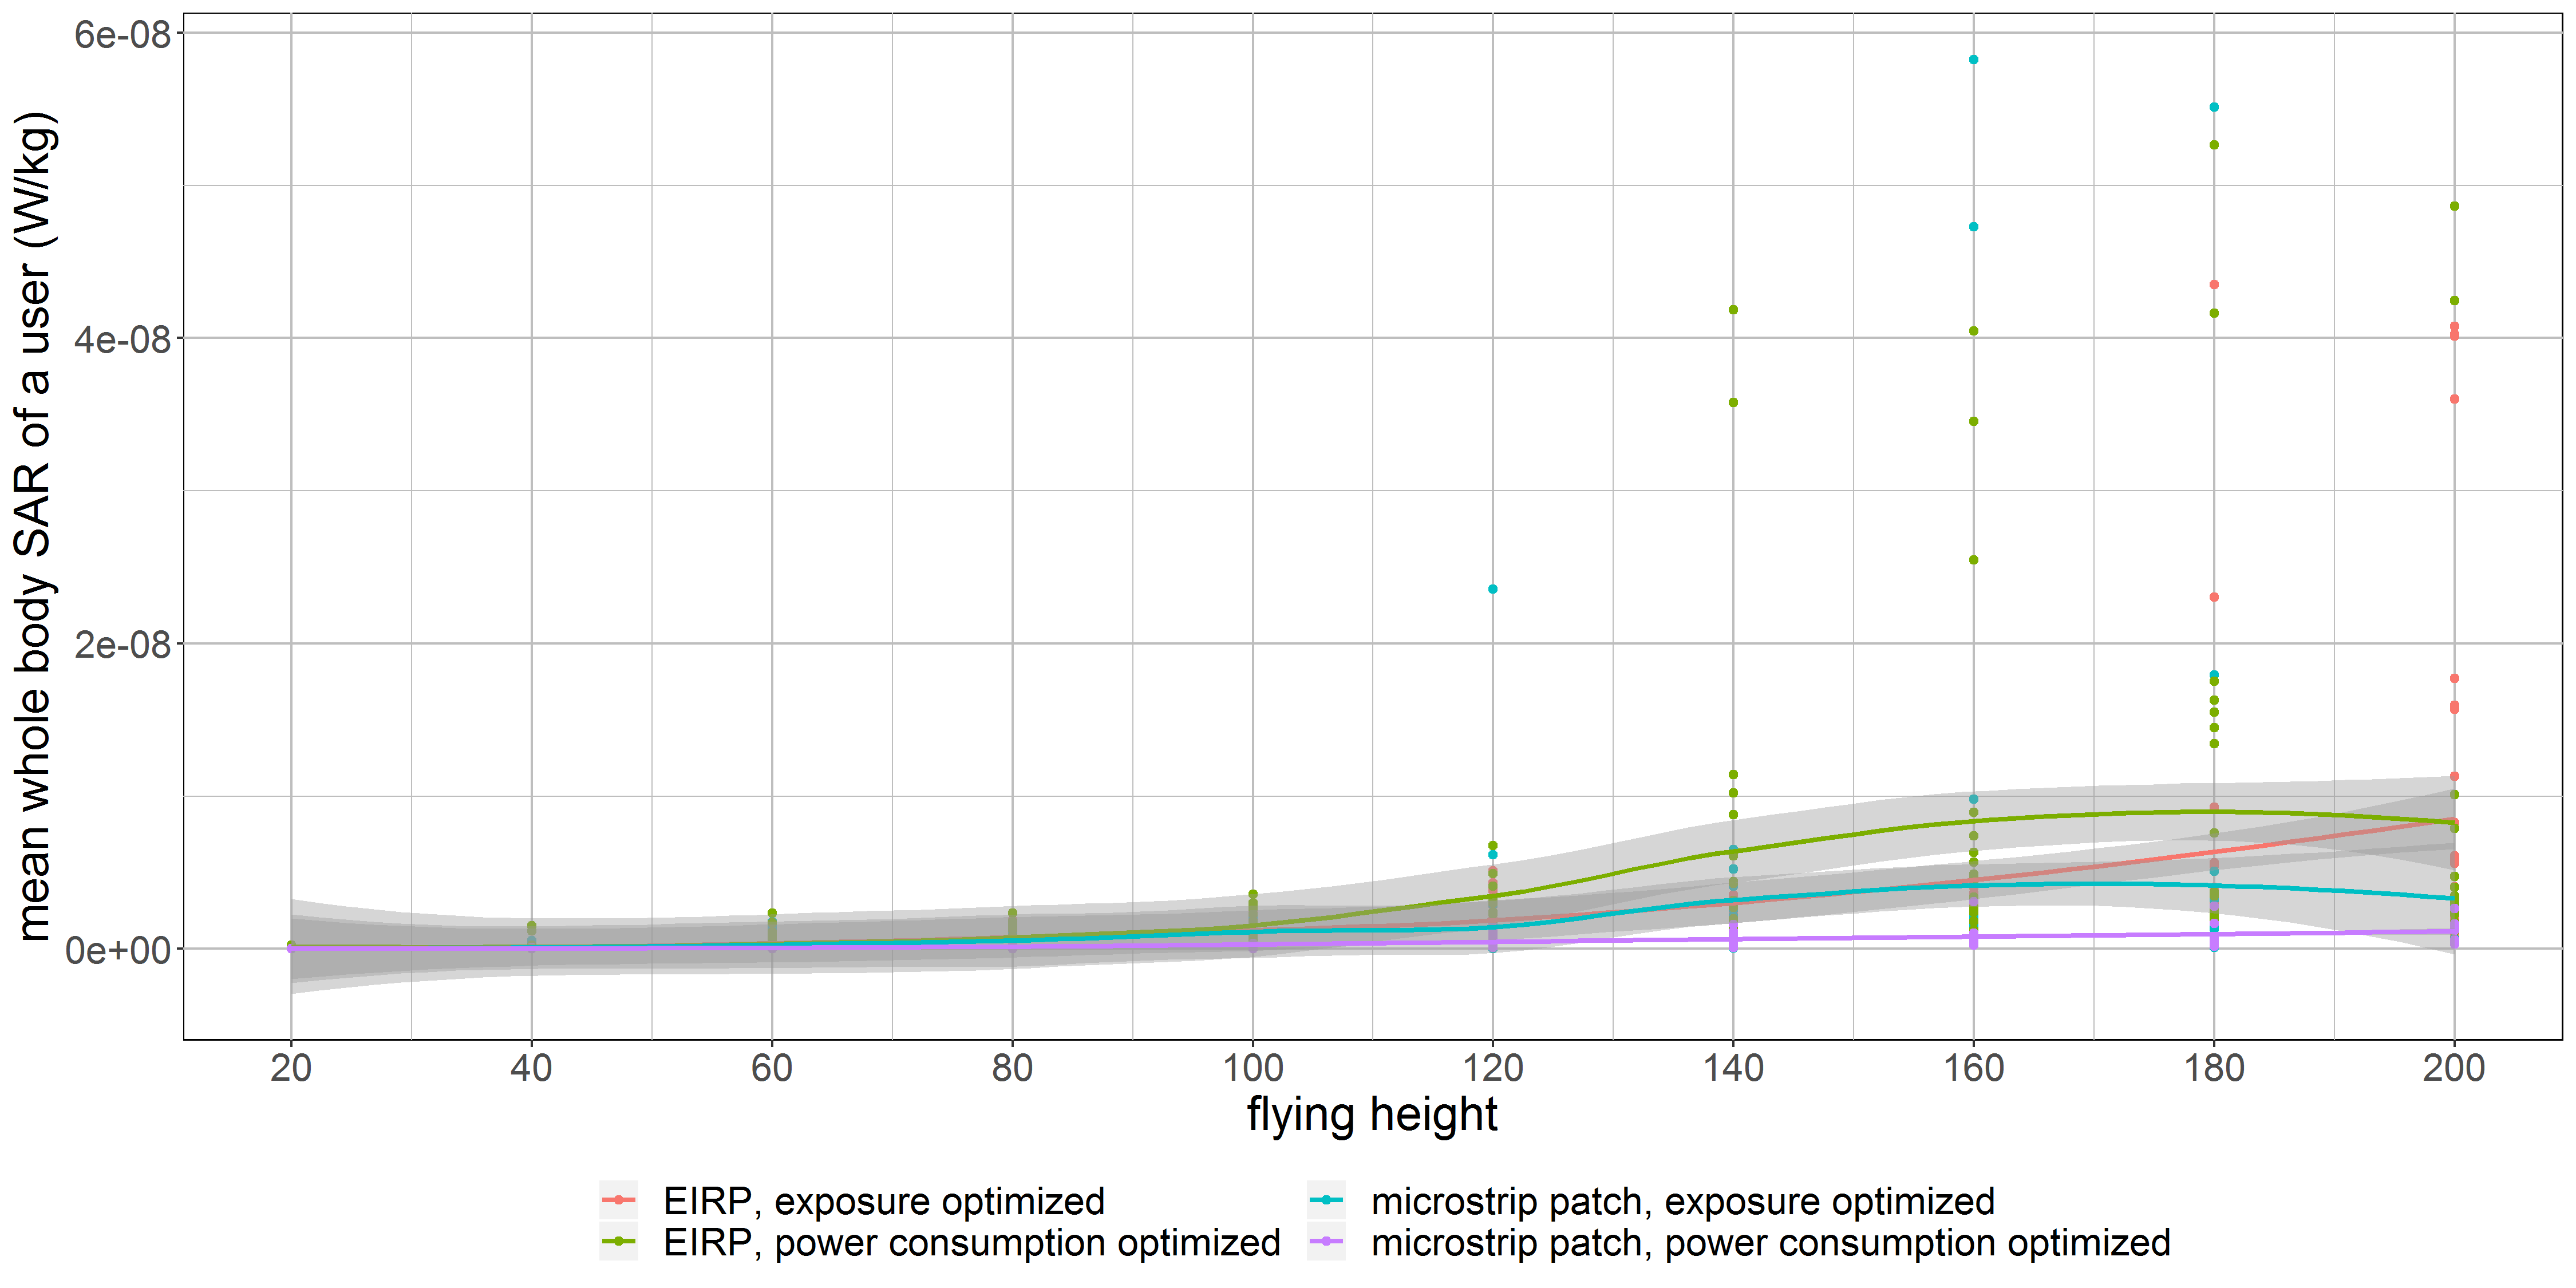
\includegraphics[width=\linewidth]{s1/fhvssar.png}
  \caption{This figure shows how SAR values from different sources are influenced by different flying altitudes.}
  \label{fig:s1_fhsar}
\end{figure}

\subsection{Increased Population with one UABS}
\subsubsection{Variable Flying Height}
A \gls{PwrC Opt} network has higher exposure compared to an \gls{Exp Opt} network; a behaviour that was already proven by \cite{J1}. 
However, for this scenario, a \gls{PwrC Opt} network will not necessarily result in a lower power consumption. 
For example, at 100 metres, an \gls{EIRP} \gls{Exp Opt} network exposes the average 
user to $1.5\ mV/m$ less but requires $20\ mW$ more.
To understand this, the behaviour of the deployment tool needs to be understood first. 
A \gls{PwrC Opt} network will result in a few high powered \gls{UABS}s because increasing the input power of an antenna costs 
less than activating a new  \gls{UAV}. Likewise, an \gls{Exp Opt} network 
generates a lot of low powered \gls{UABS}s because the lower the power of the antenna, the lower the exposure. This has the consequence that the cover radius 
is less and therefore requires more \gls{UAV}s which costs more energy.
When only a limited amount of \gls{UABS}s are available, 
like only one in this scenario, the tool will only keep \gls{UABS}s which cover the most users. 
Therefore, the power consumption in a \gls{PwrC Opt} network is often higher. 
\begin{figure}[h!]
  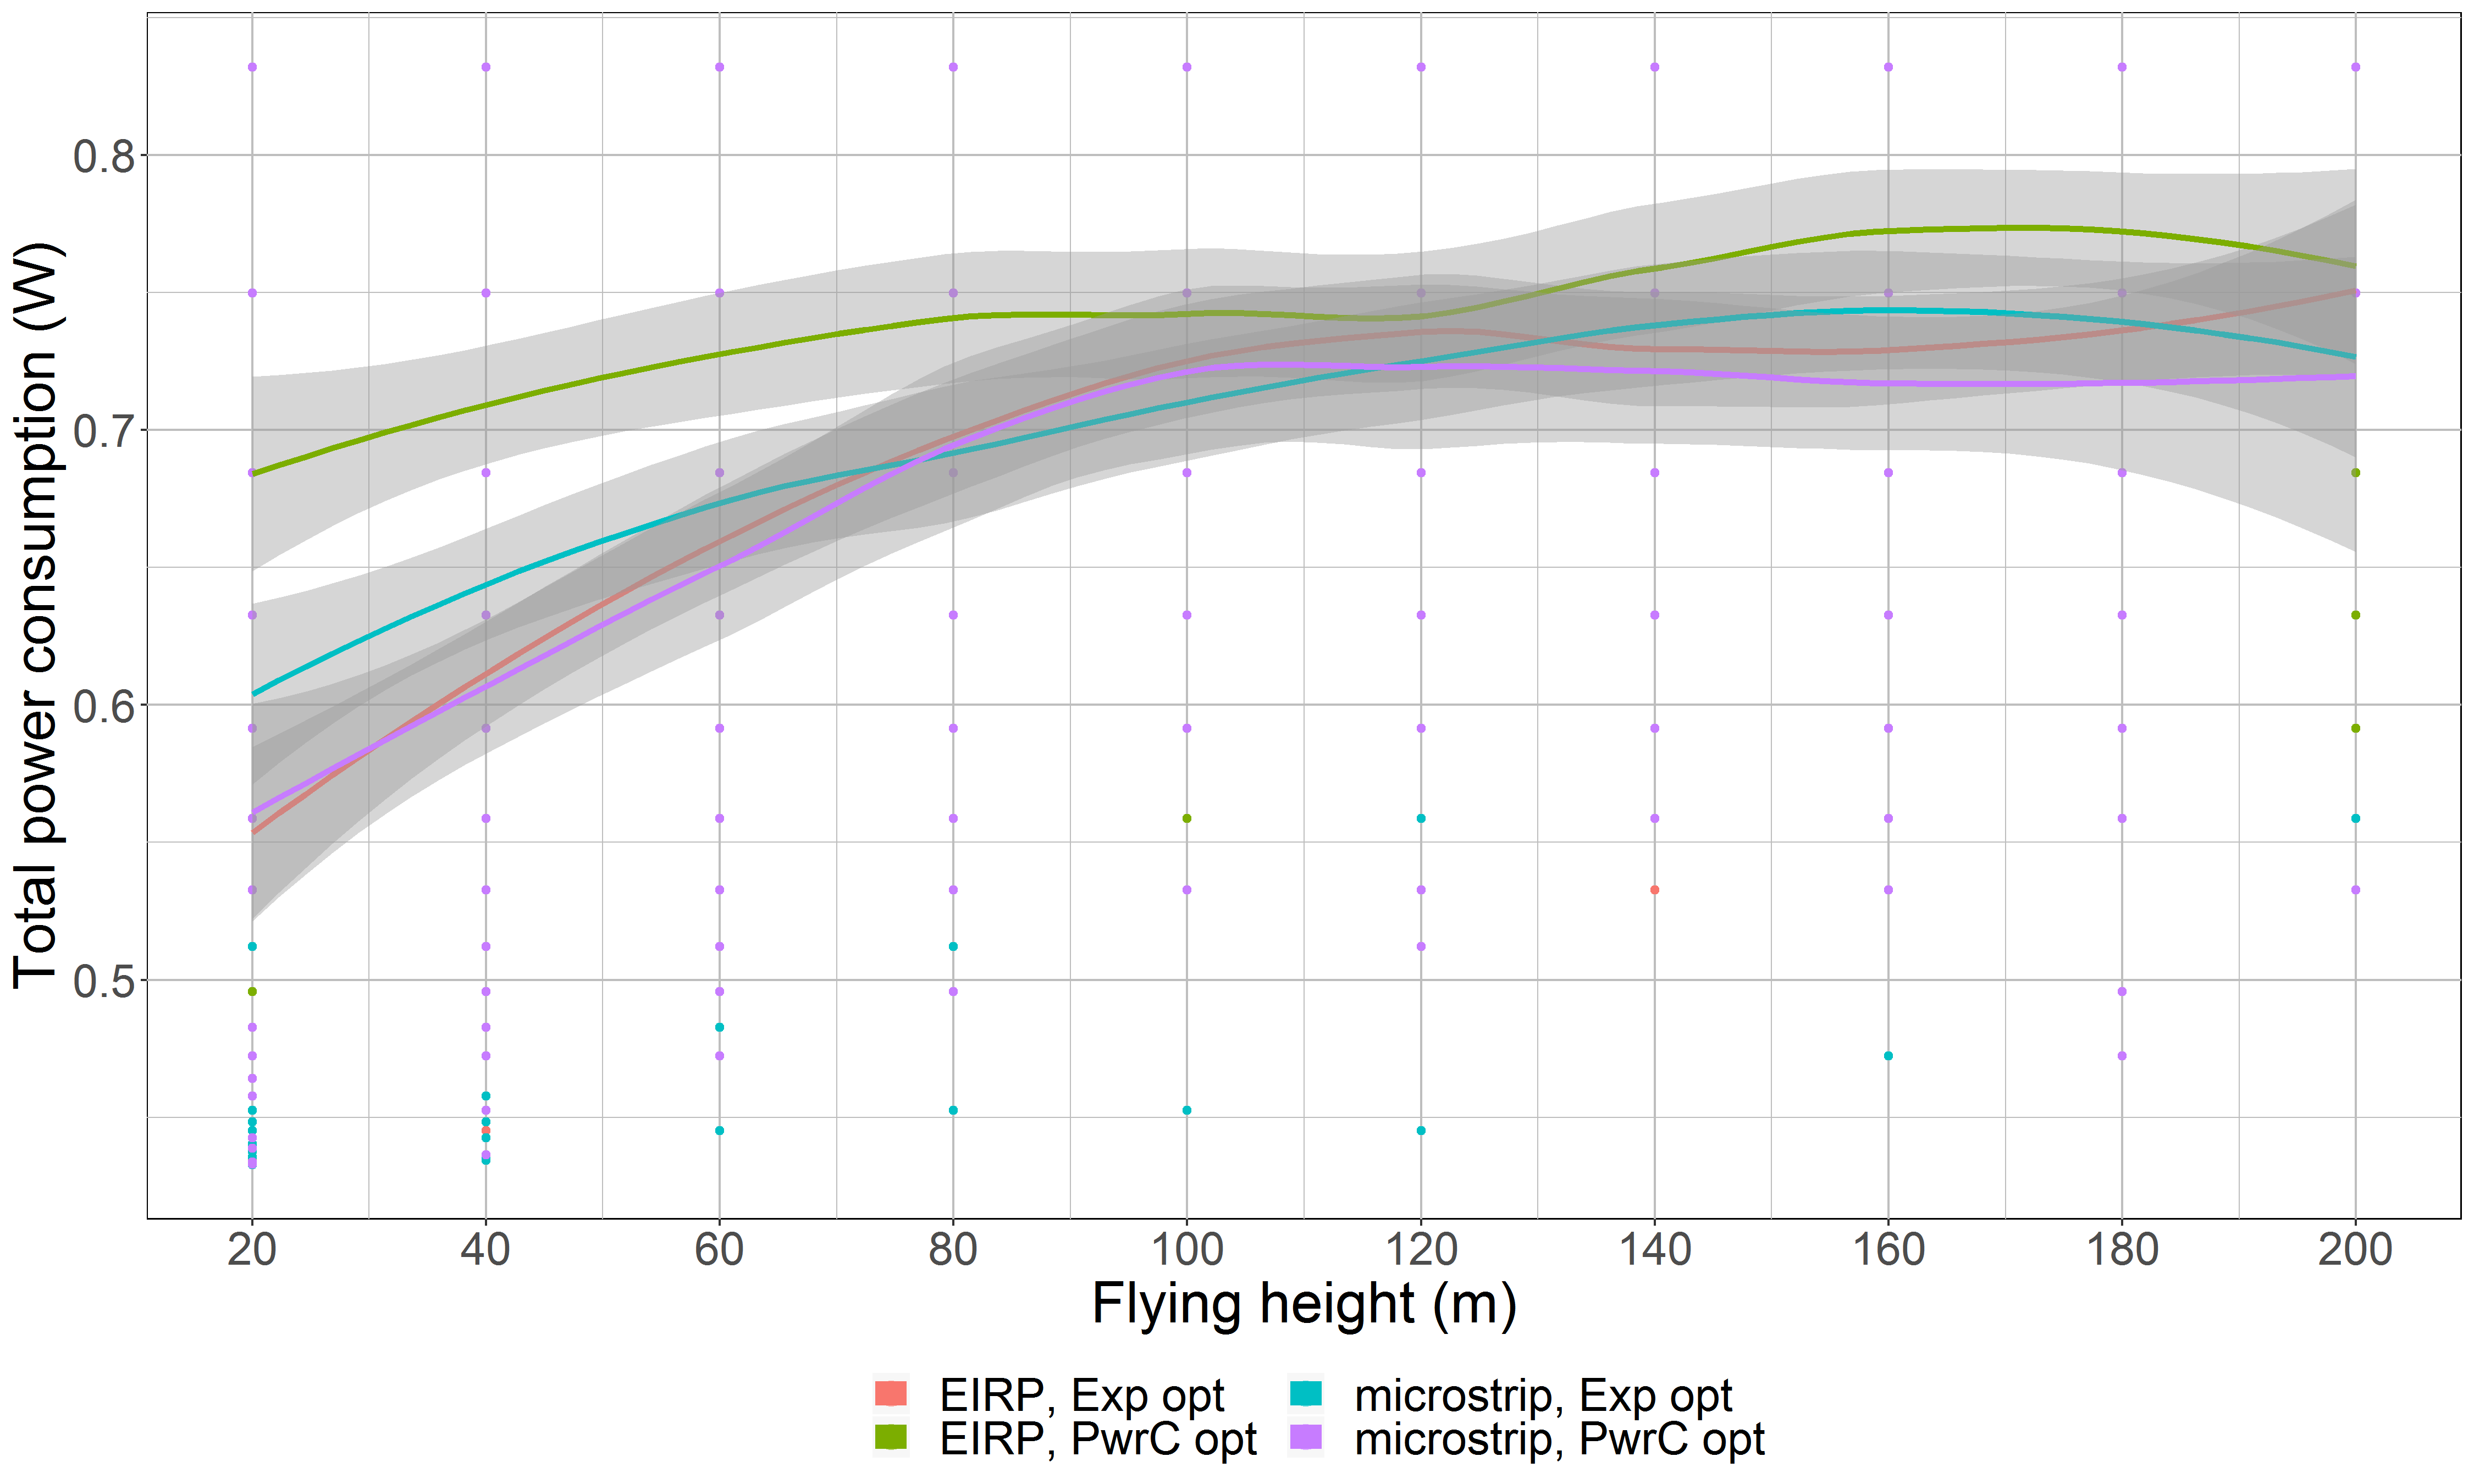
\includegraphics[width=\linewidth]{s2/fhvsdlAndPc.png}
  \caption{Fig. (a) show how the flying height influences the downlink electromagnetic radiation of the average user and fig. (b) the
  power consumption of the entire network for the only \acs{UABS} available in the network.}
  \label{fig:s2a_dlAndPc}
\end{figure}

Further, figure \ref{fig:s2a_dlAndPc} also show that the exposure increases with higher flying altitudes
because there is a lower probability of having \gls{NLOS} links by obstructing buildings. This has as consequence that  
more users become covered. 
Increasing the flying height from 20 to 100 metres improves the coverage between 1\% and 2\% for all four configurations.
The increasing electromagnetic radiation is however not unlimited.
A microstrip \gls{PwrC Opt} network is at his highest point  
around 162 metres and an \gls{EIRP} \gls{PwrC Opt} is at his highest at 195 metres.
This decline starts later for exposure optimized networks and is situated outside the investigated flying range.
The decreasing electromagnetic radiation at high flying altitudes is not caused by the obstructing buildings but by the 
distance in general.

Figure \ref{fig:s2shfourSourcesMatrix} shows the whole body $SAR_{10g}$ for the weighted average user, deducted from all electromagnetic sources. 
When investigating the three different sources, we see 
that the $SAR^{myUABS}$ shows the same curve as it did with the electromagnetic exposure 
in figure \ref{fig:s2a_dlAndPc}.a. This is normal behaviour considering that equation \ref{eq:DLconversion} is able of 
converting the \gls{DL} exposure to \gls{SAR} by simply multiplying with a constant.
During the entire time is $SAR^{myUABS}$ the most dominant factor followed by 
 the near-field radiation from the user's own device.
The far-field radiation from other \gls{UE} barely has influence. 
As an illustration, when the \gls{UABS} flies at 140 metres, the average user in an \gls{EIRP} \gls{PwrC Opt} network will 
experience around  2.1 $nW/kg$ from the \gls{UABS} and around 0.2 $nW/kg$ from his own device.
The exposure from other \gls{UE} can be neglected with 0.03 $pW/kg$. A low but plausible value considering that most 
\gls{UE} are not radiating anything since they are uncovered.

\begin{figure}[h!]
  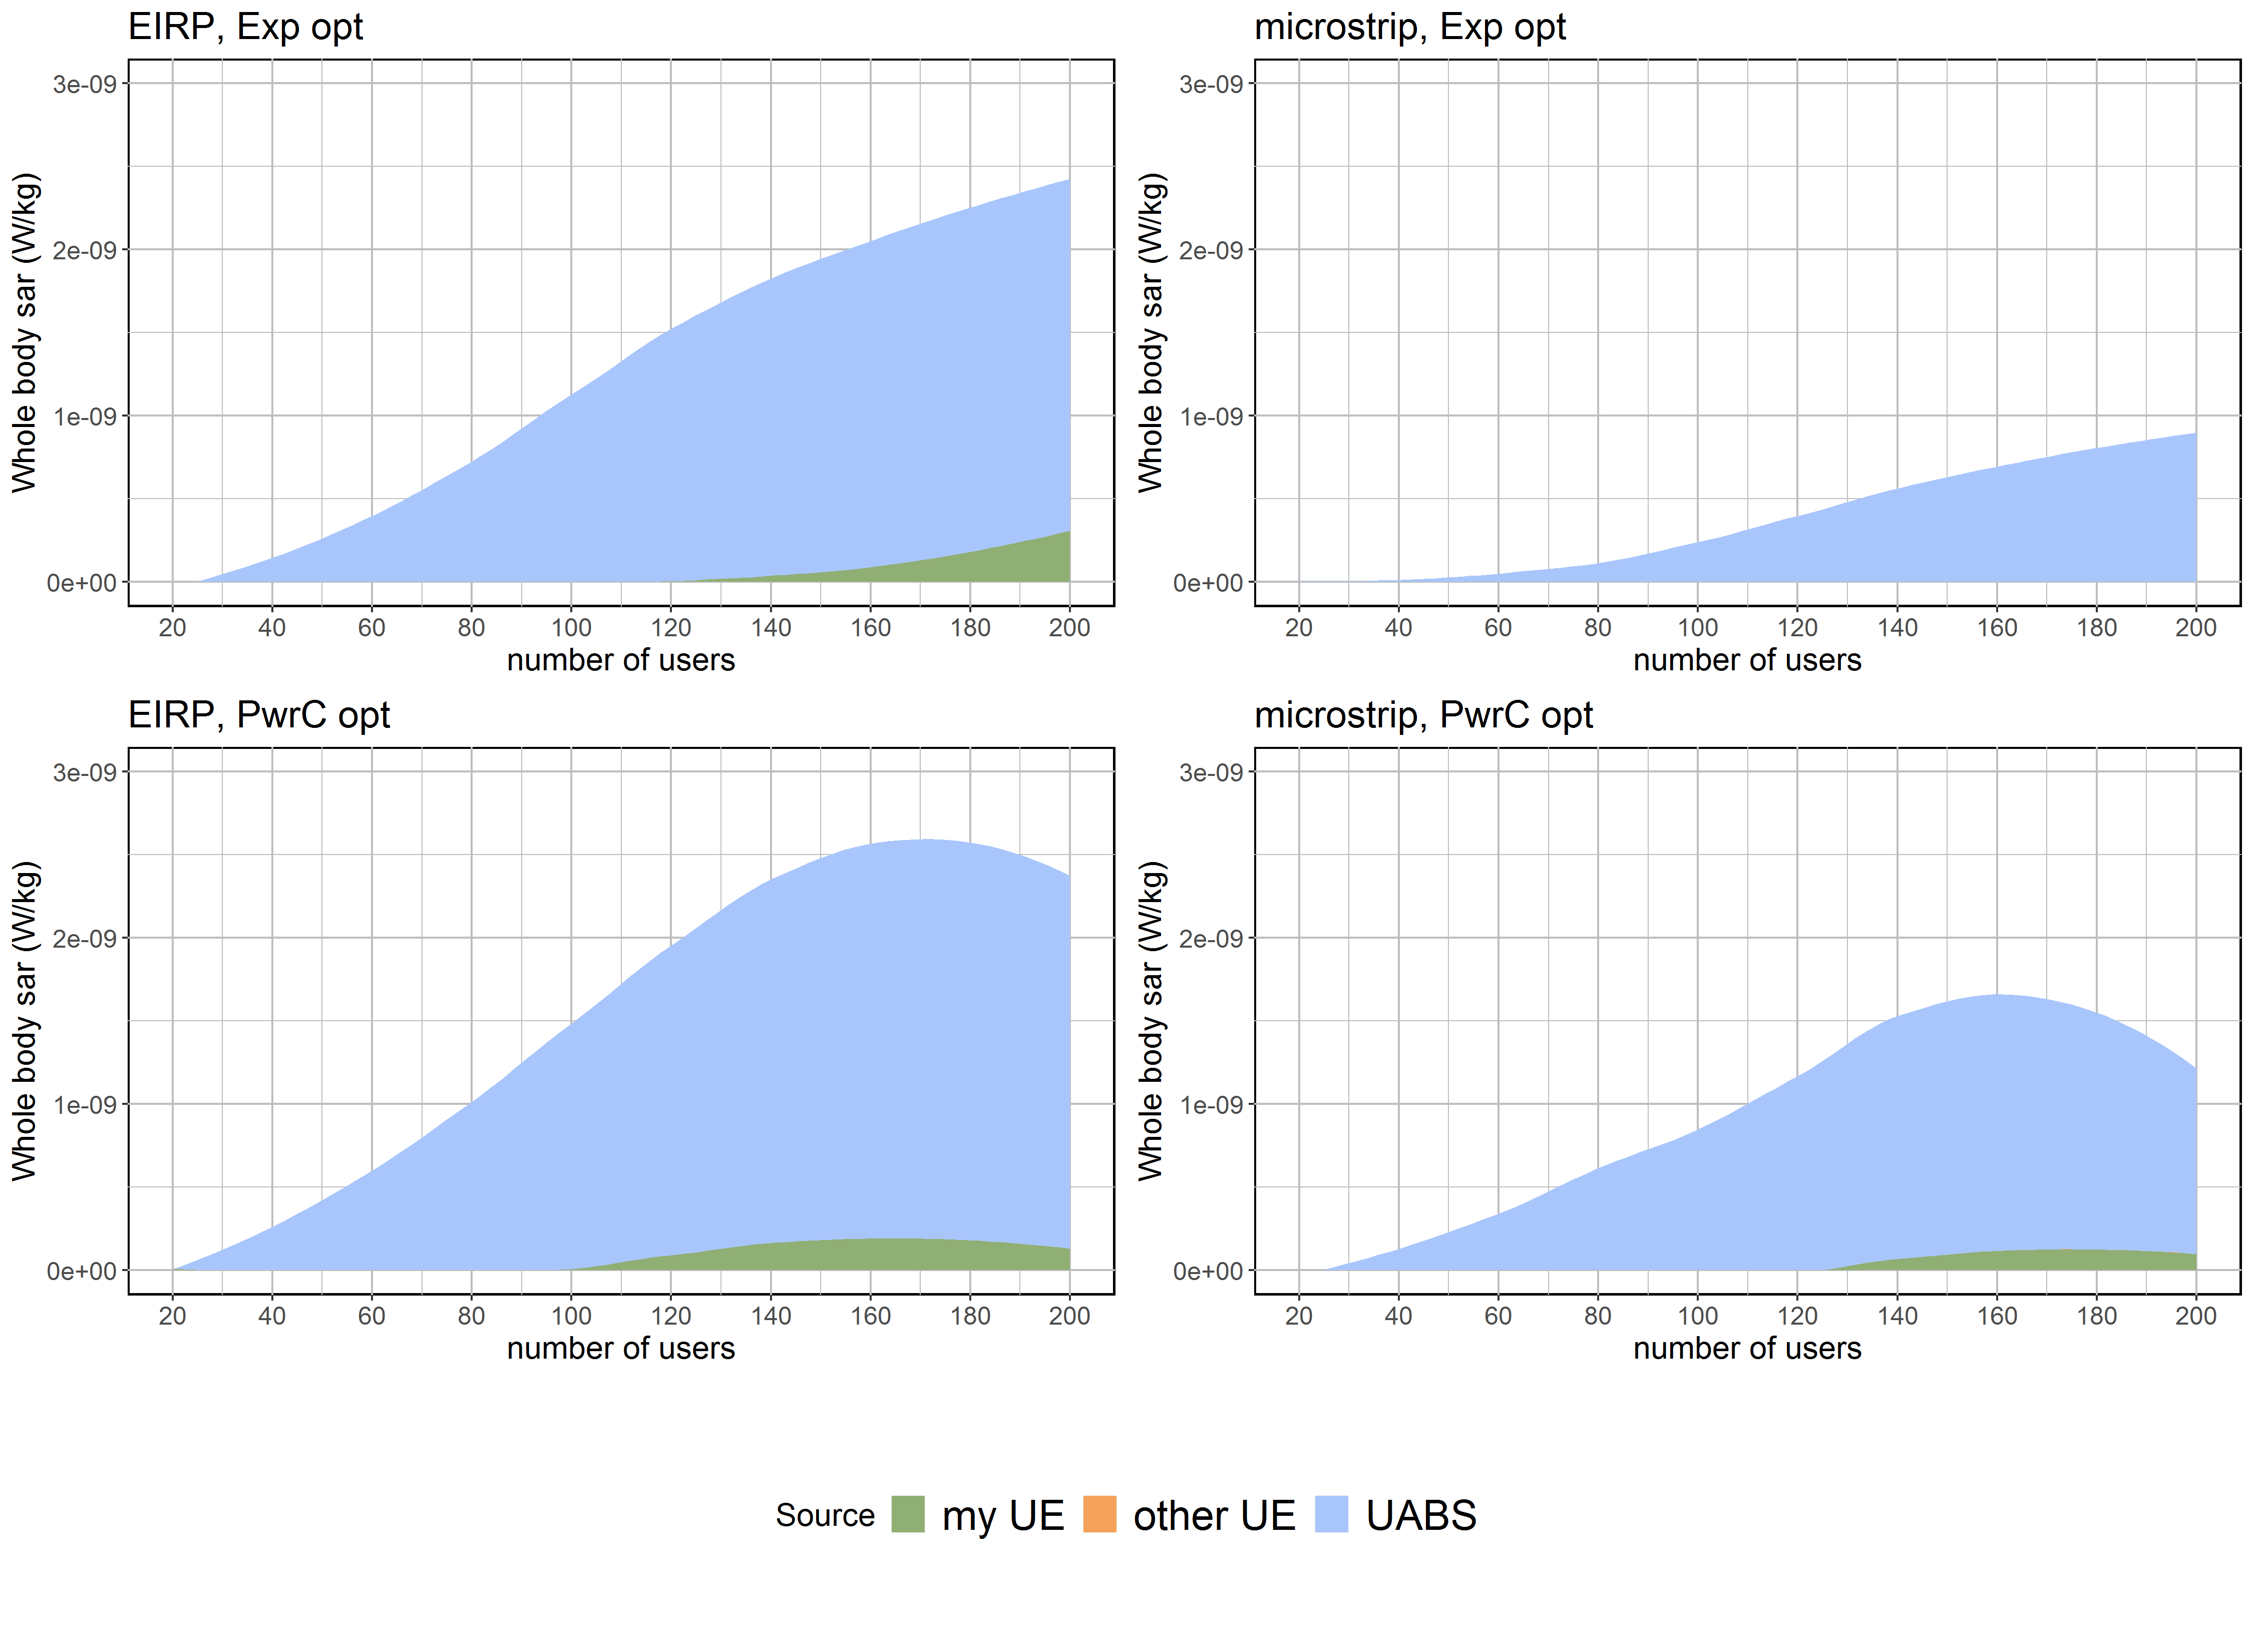
\includegraphics[width=\linewidth]{s2/fhFourSources.png}
  \caption{Each figure corresponds with a certain configuration and shows how the \acs{SAR} from 
  different sources are influenced by an increasing flying height.}
  \label{fig:s2shfourSourcesMatrix}
\end{figure}

\subsubsection{Variable Number of Users}
The number of covered users increases linearly compared to the number of users present in the network as shown in figure 
\ref{fig:s2uvsnumcovusers}.b. It illustrates how an \gls{isotropicradiator} is able to reach more users 
compared to a microstrip patch antenna. Just like an power consumption optimized network 
is able to reach more users than an exposure optimized network.
For example, with 600 users, 5 to 7 additional 
people can be covered when replacing a microstrip patch antenna with an \gls{isotropicradiator}
and changing an exposure optimized network with an power consumption optimized network will 
cover one or two additional users.
\begin{figure}[h!]
  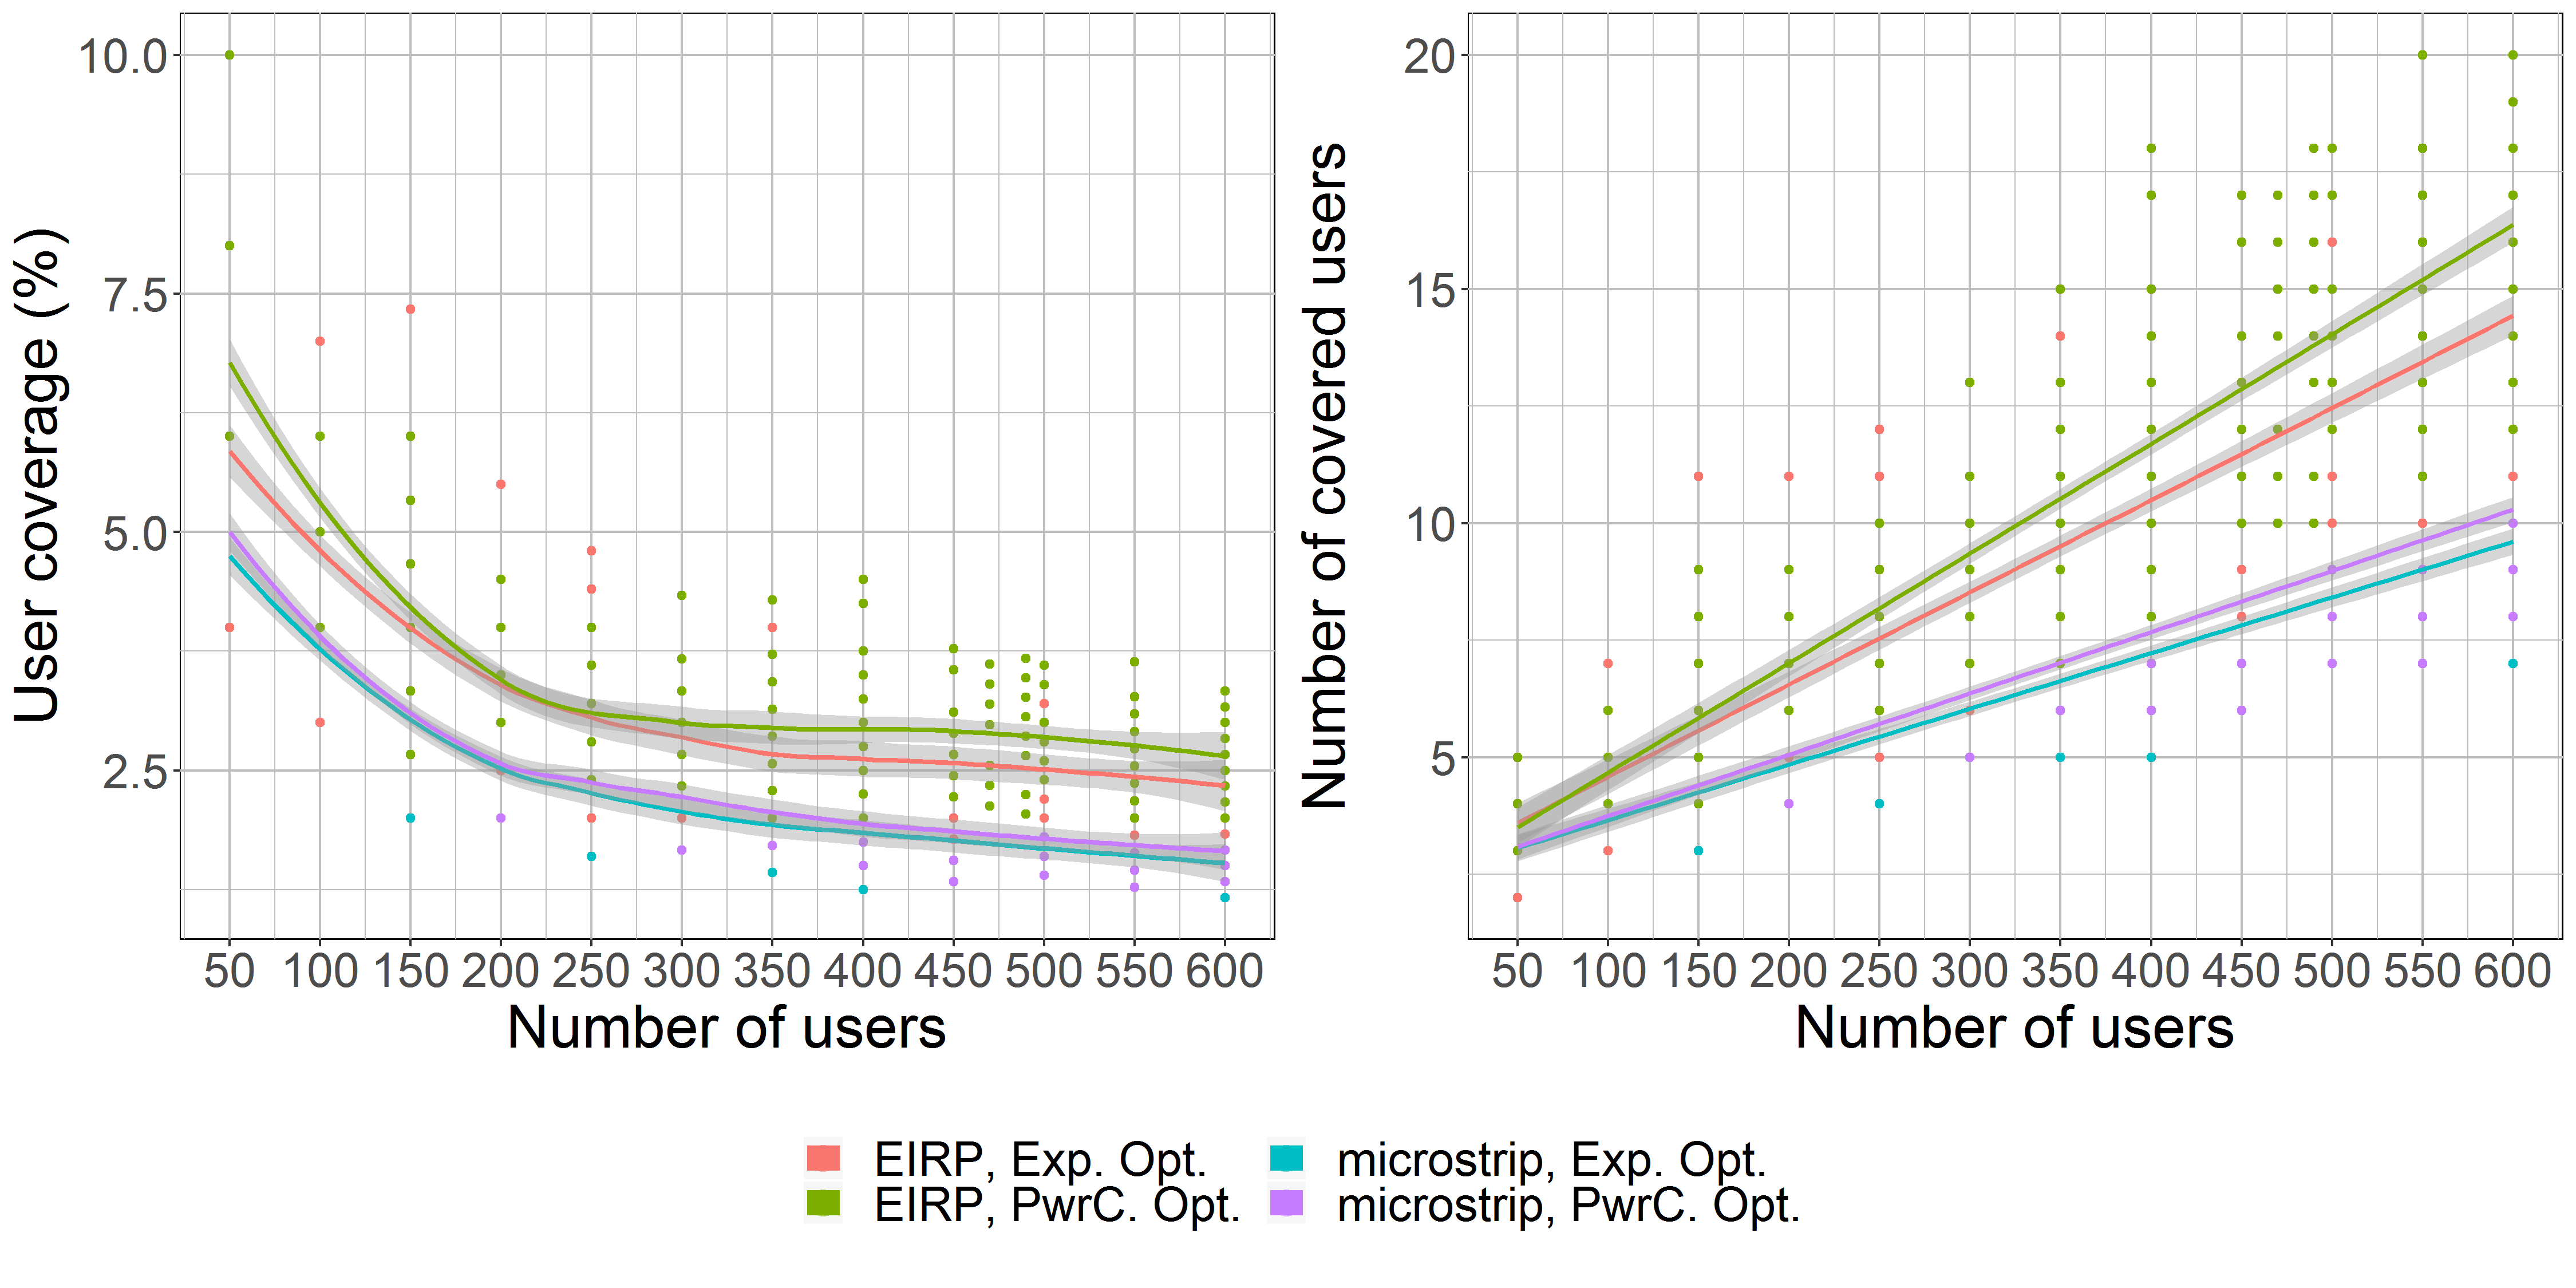
\includegraphics[width=\linewidth]{s2/uvsnumdronesAndCov.png}
  \caption{The influence of increasing traffic on the user coverage.}
  \label{fig:s2uvsnumcovusers}
\end{figure}

Figure  \ref{fig:s2b_dlAndPc}.a  is influenced by  \ref{fig:s2uvsnumcovusers}.a. When less users are 
covered, the exposure of the average user will decrease as well.
For example, in an EIRP \gls{PwrC Opt} network, 50 users have a 6.75\% coverage which corresponds with a weighted average exposure of  18 $mV/m$
while 600 users with 2.75\% coverage only have 9 $mV/m$.
Further,  figure \ref{fig:s2b_dlAndPc}.b is directly influence by figure \ref{fig:s2uvsnumcovusers}.b. When the \gls{UABS} has to cover more users,
the probability that some of these users have a worse path loss is higher. The \gls{UABS} solves this problem by increasing the 
power consumption. Increasing the population from 50 to 600 will require between 0.05 and 0.1 $W$ more. 
For this scenario, no clear difference in power consumption exists between the four configurations.

\begin{figure}[h!]
  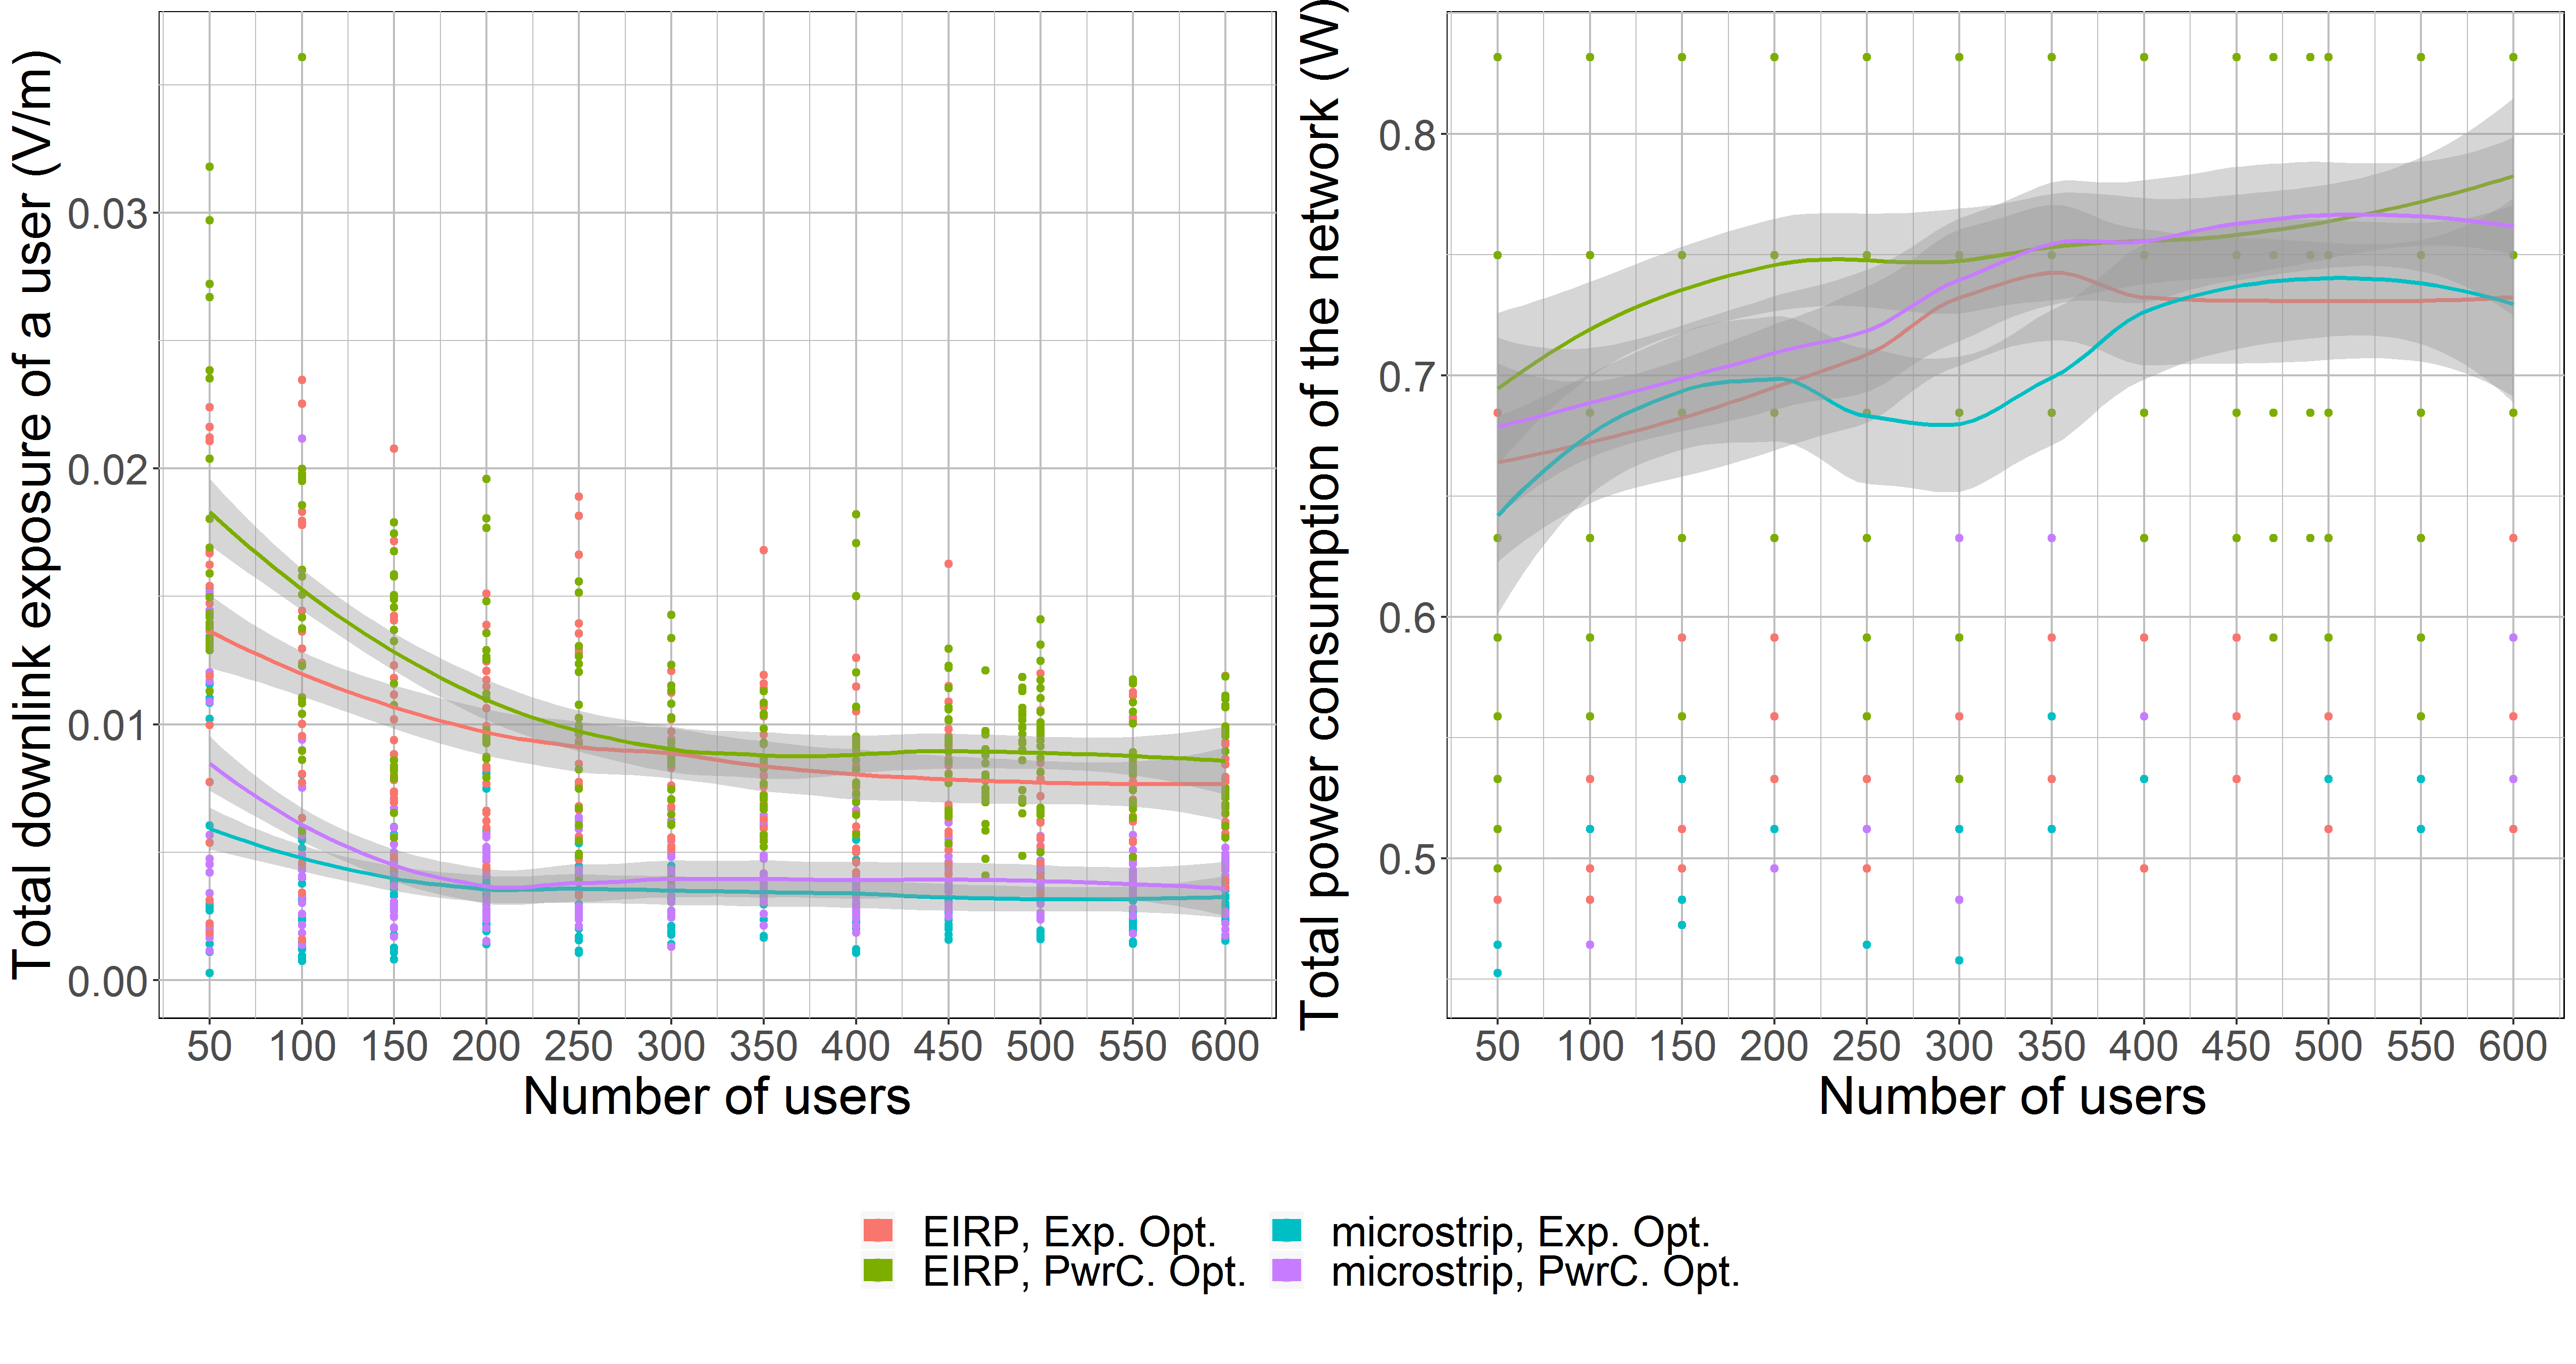
\includegraphics[width=\linewidth]{../results/s2/uvsdlAndPc.png}
  \caption{These two figures show how various sizes of population influence the downlink electromagnetic radiation of the average user (left) and 
  power consumption of the entire network (rights) for one \acs{UABS} available in the network.}
  \label{fig:s2b_dlAndPc}
\end{figure}

The \gls{SAR} comming from the 
users own device is on average zero since most users are uncovered. 
Figure \ref{fig:uvsulsarcentralUsers} shows the exposure for the covered user
just below the \gls{UABS}. Scenario I already showed that the \gls{SAR} from the user's own device is only influenced by the flying height
and is also confirmed by the results in fig. \ref{fig:uvsulsarcentralUsers} where constant $SAR^{myUE}$ is measured of 0.15 $\mu W/kg$.
The \gls{SAR} from the \gls{UABS} experiences a slight increase of 0.005 $\mu W/kg$. When the population grows, more users
will be near the \gls{UABS}. The \gls{UABS} will likely decide to cover these users as well as visible in figure \ref{fig:connectionMap}.
These users might have a slightly 
worse path loss because of obstructing buildings or somewhat bigger distance. The \gls{UABS} reacts to this by increasing 
his power consumption causing an increase in the \gls{DL} \gls{SAR} for the central user.
The far-field radiation from \gls{UE} is very low as mentioned before and therefore added separately in figure \ref{fig:connectionMap}.b.
It shows that the \gls{SAR}  from other \gls{UE} increases from zero to $0.15\ pW/kg$. This is normal 
behaviour considering that around the central user more and more people become available of which some will be connected to the \gls{UABS}
and therefore also emitting radiation.

\begin{figure}[!htb]
\minipage{0.50\linewidth}
  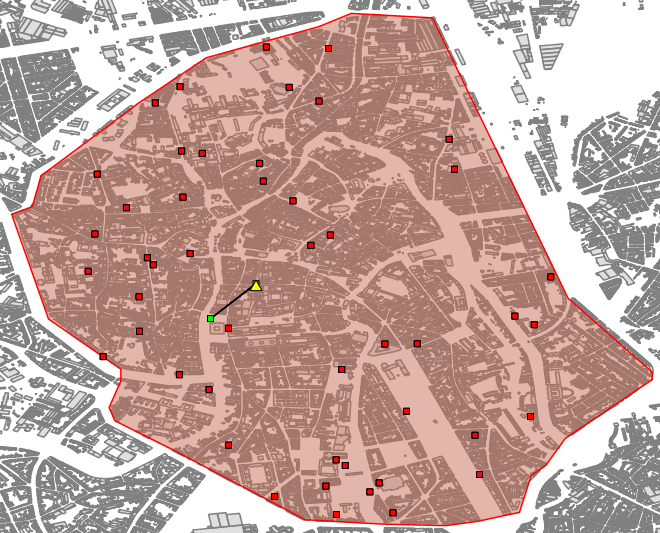
\includegraphics[width=\linewidth]{../images/connectionsMap50Users.png}
\endminipage\hfill
\minipage{0.50\linewidth}%
  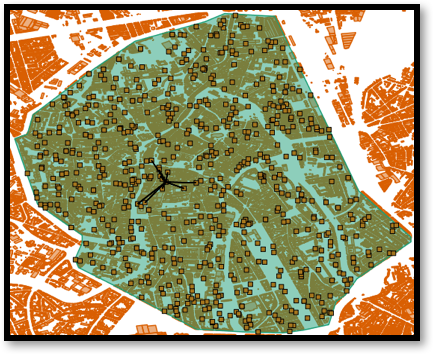
\includegraphics[width=\linewidth]{../images/connectionsMap600Users.png}
\endminipage
  \caption{Overview of which users are connected to the \gls{UABS}. The map on the left is for 50 active users while the map on the right considers 600 active users.}
  \label{fig:connectionMap}
\end{figure}

\begin{figure}[h]
\centering
  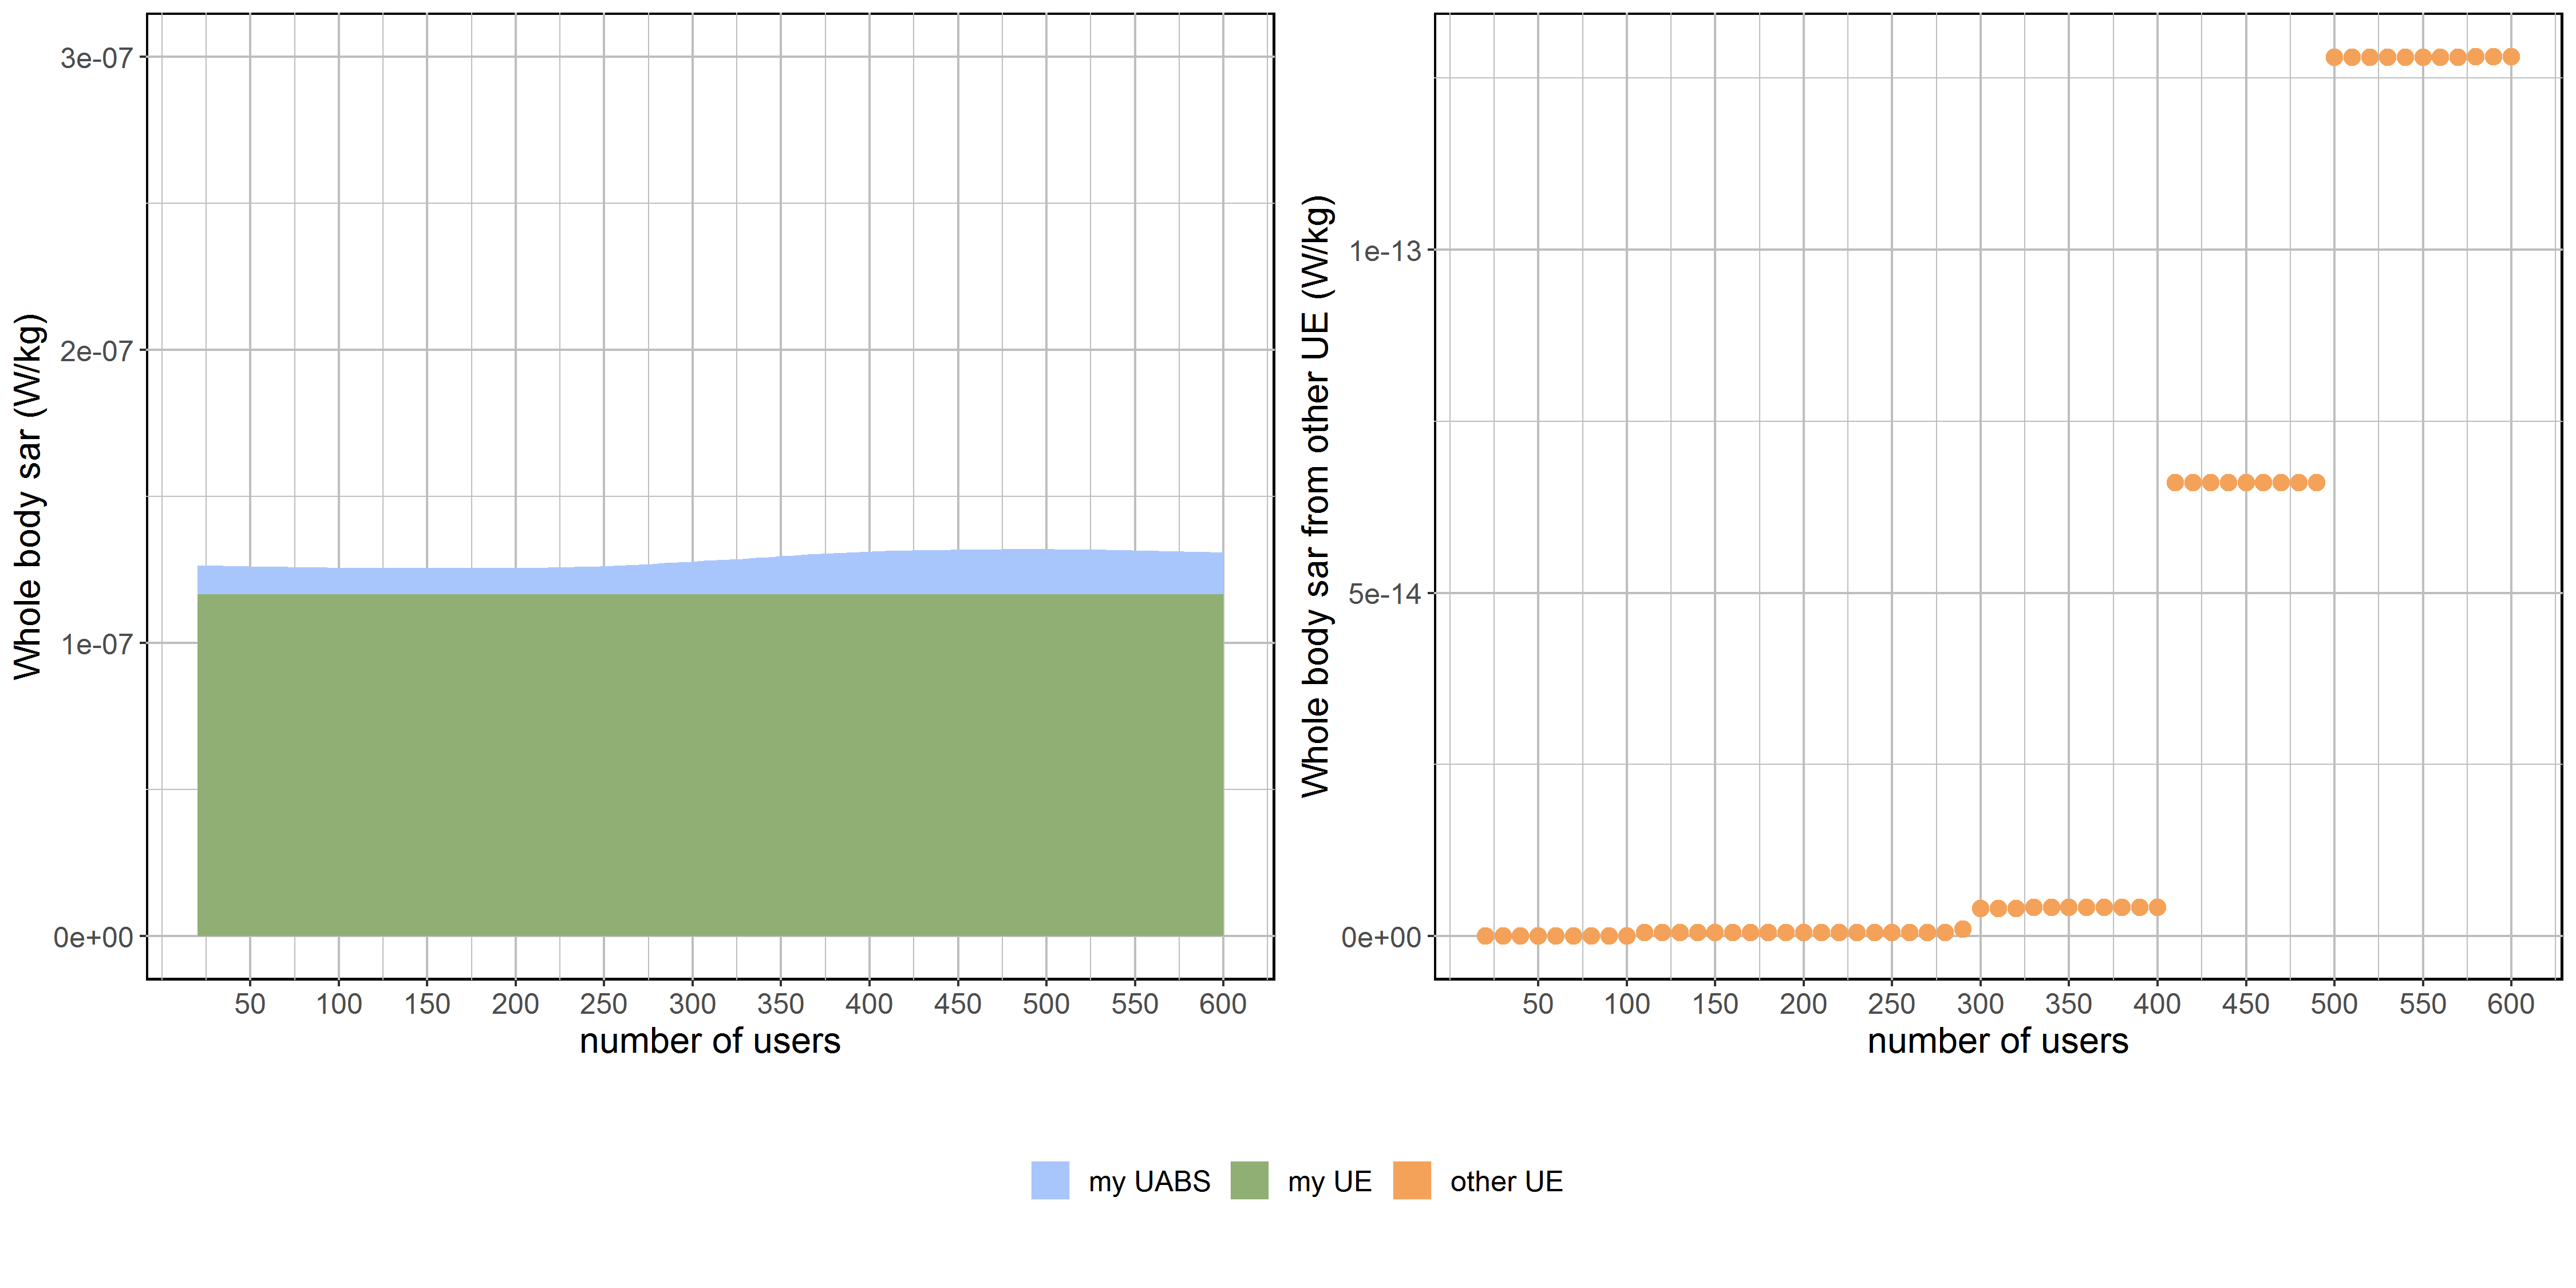
\includegraphics[width=0.9\linewidth]{../results/s2/uvsulsarcentralUser.png}
  \caption{SAR-values for the user who is directly beneath the only \acs{UABS} available.}
  \label{fig:uvsulsarcentralUsers}
\end{figure}

\FloatBarrier
\subsection{Unlimited Number of UABSs}
\subsubsection{Variable Flying Height}
The same scenario as in the previous section is investigated. Only now, an unlimited number of \gls{UABS}s is available.
The results prove that the different optimization strategies work as intended.
A \gls{PwrC Opt} network has indeed a lower power consumption but therefore result in higher electromagnetic radiation.
On the other hand, an \gls{Exp Opt} network will reduce the electromagnetic exposure by using more \gls{UAV}s and thence also increase the network's
power consumption. This conclusion was already made in \cite{J1} and is supported by these results.
For example, when comparing both optimization strategies for the same \gls{isotropicradiator} and the same default flying height, we see that
the power consumption optimized network requires 51 $W$ and therefore exposes its users
to $15\ mV/m$. When optimizing towards electromagnetic radiation, the exposure drops to $11.5\ mV/m$ but at a cost of a higher power consumption
of $54\ W$.
\begin{figure}[h!]
  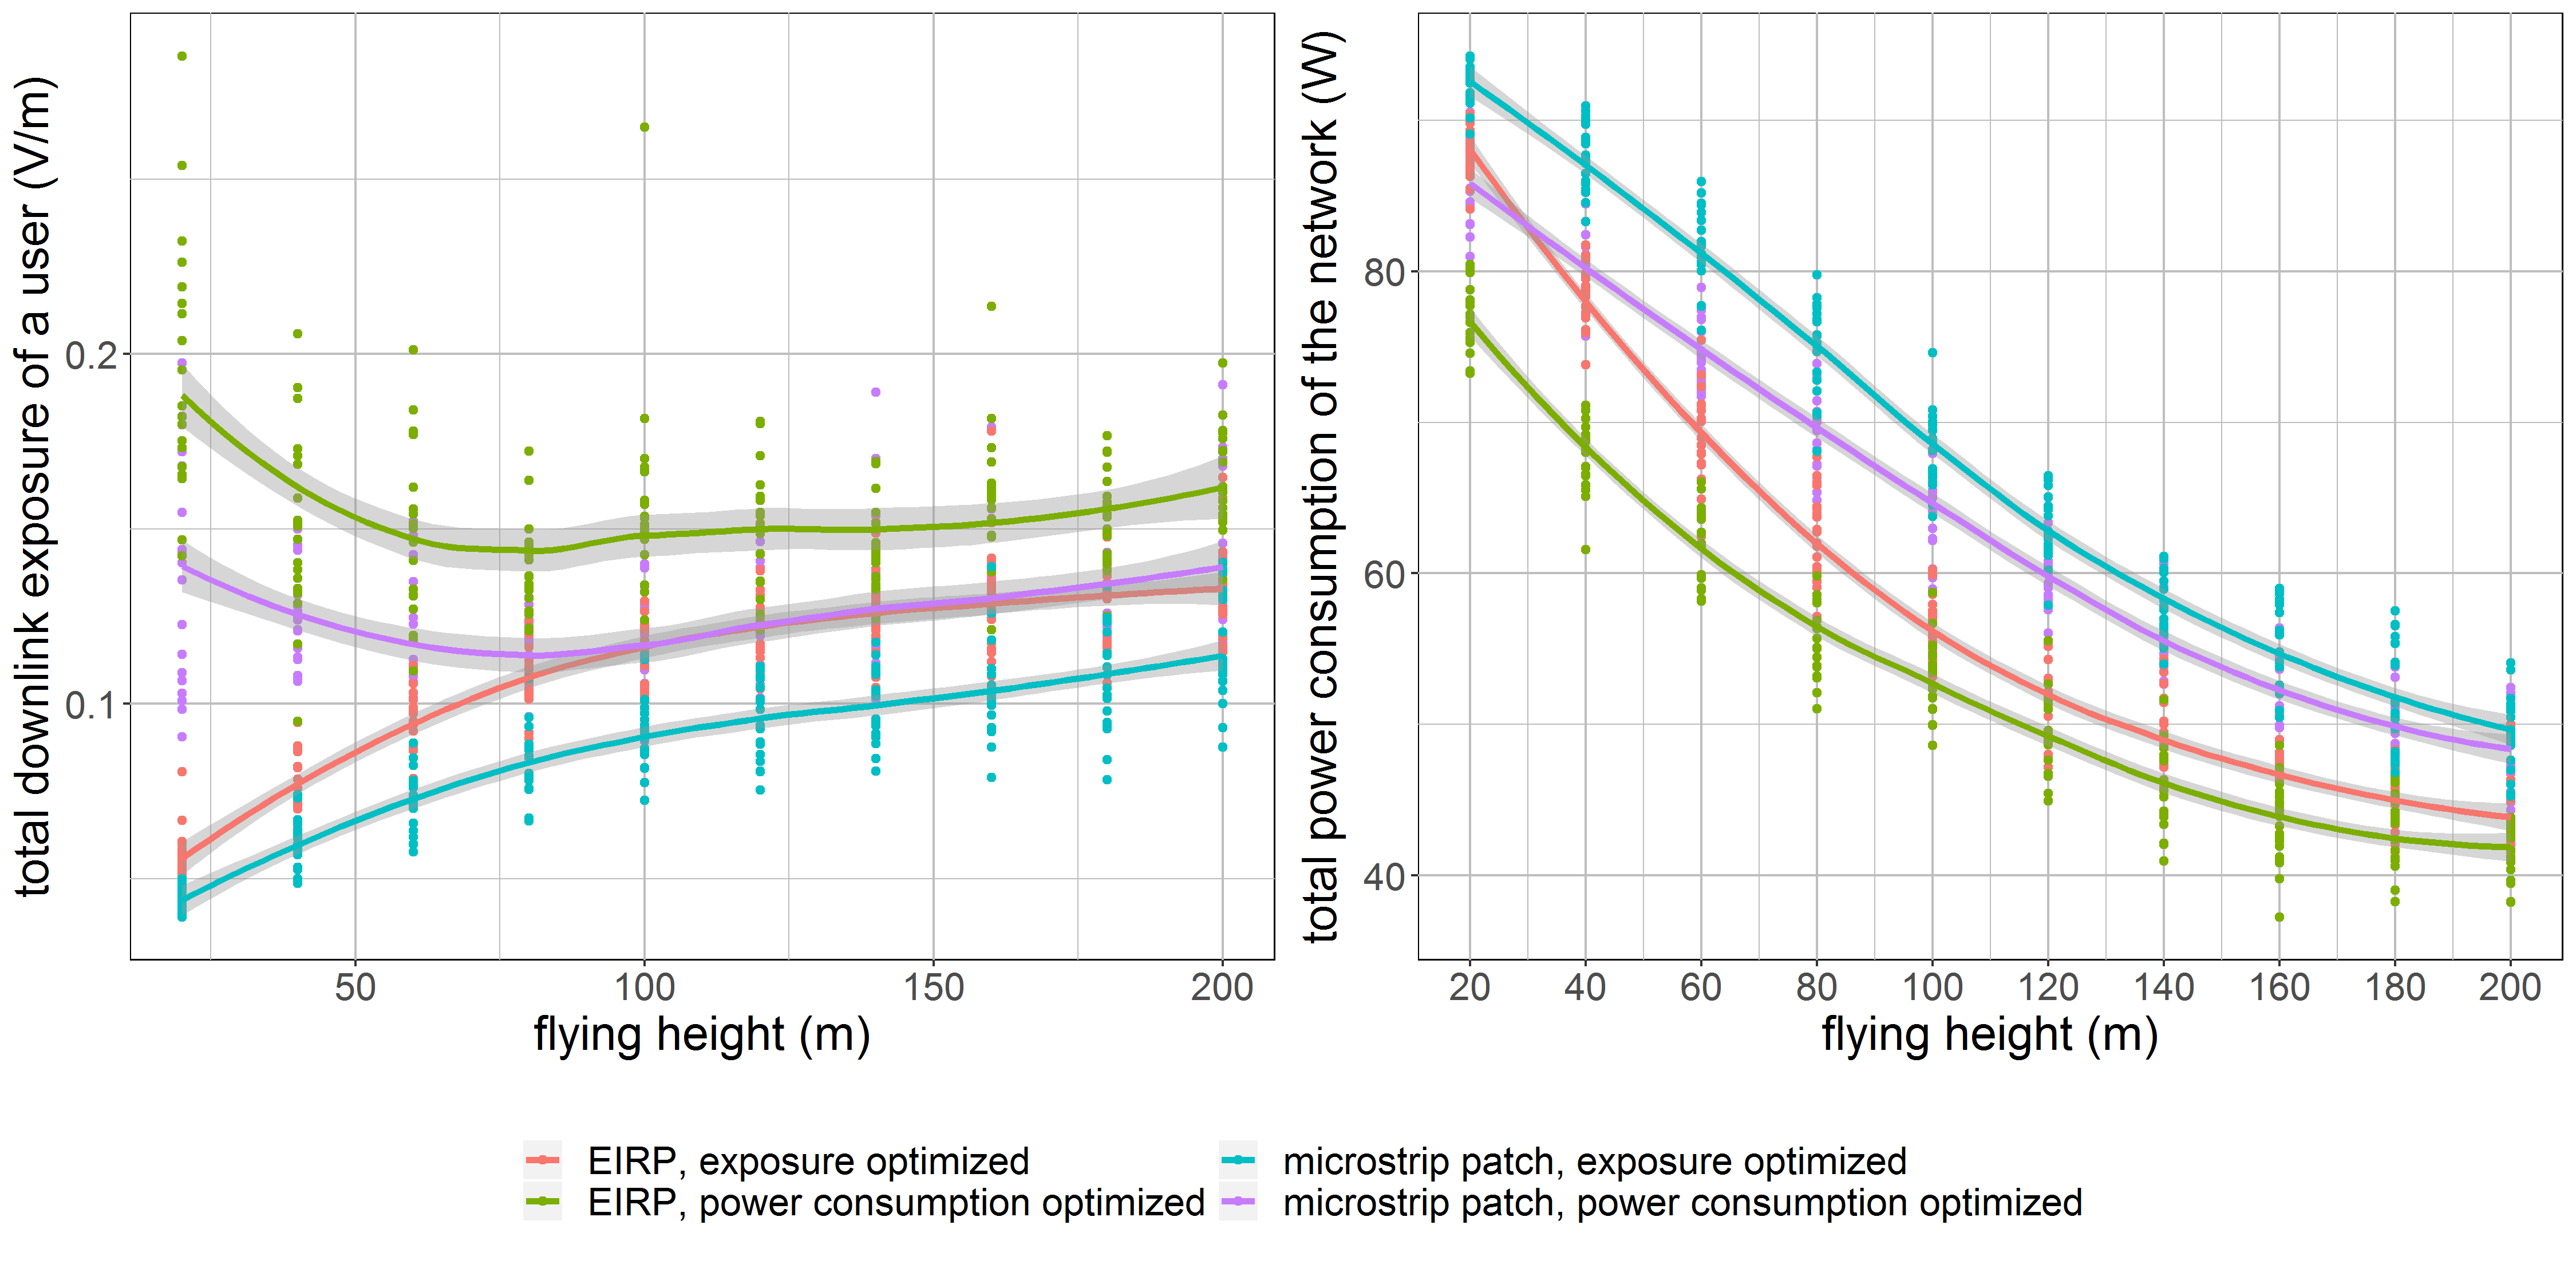
\includegraphics[width=\linewidth]{../results/s3/fhvsdlAndPc.png}
  \caption{These two figures show how the flying height influences the downlink electromagnetic radiation of the average user (left) and 
  power consumption of the entire network (right) for an unlimited number of drones.}
  \label{fig:s3a_dlAndPc}
\end{figure}

The exposure in figure \ref{fig:s3a_dlAndPc} shows that an \gls{Exp Opt} network increases logarithmically while the \gls{PwrC Opt} network rather 
has a concave relationship with the flying height, and has its lowest point at around 70 metres.

Figure \ref{fig:s3a_numDronesAndCov}.a shows that the optimal coverage is achieved at a low flying height of 
40 metres with around 99\% coverage. 
However, there is a downside to this. 
Figure \ref{fig:s3a_numDronesAndCov}.b 
 shows that the number of required \gls{UAV}s increases when the flying altitude becomes lower;
a behaviour which was also determined in \cite{J2}.
For example, an microstrip \gls{Exp Opt} network and an \gls{EIRP} \gls{PwrC Opt} network require respectively 84 and 64
\gls{UABS}s at a flying altitude of $200\ m$ which increases respectively to 211 and 162 \gls{UABS}s at a much lower flying altitude of $20\ m$.

\begin{figure}[]
  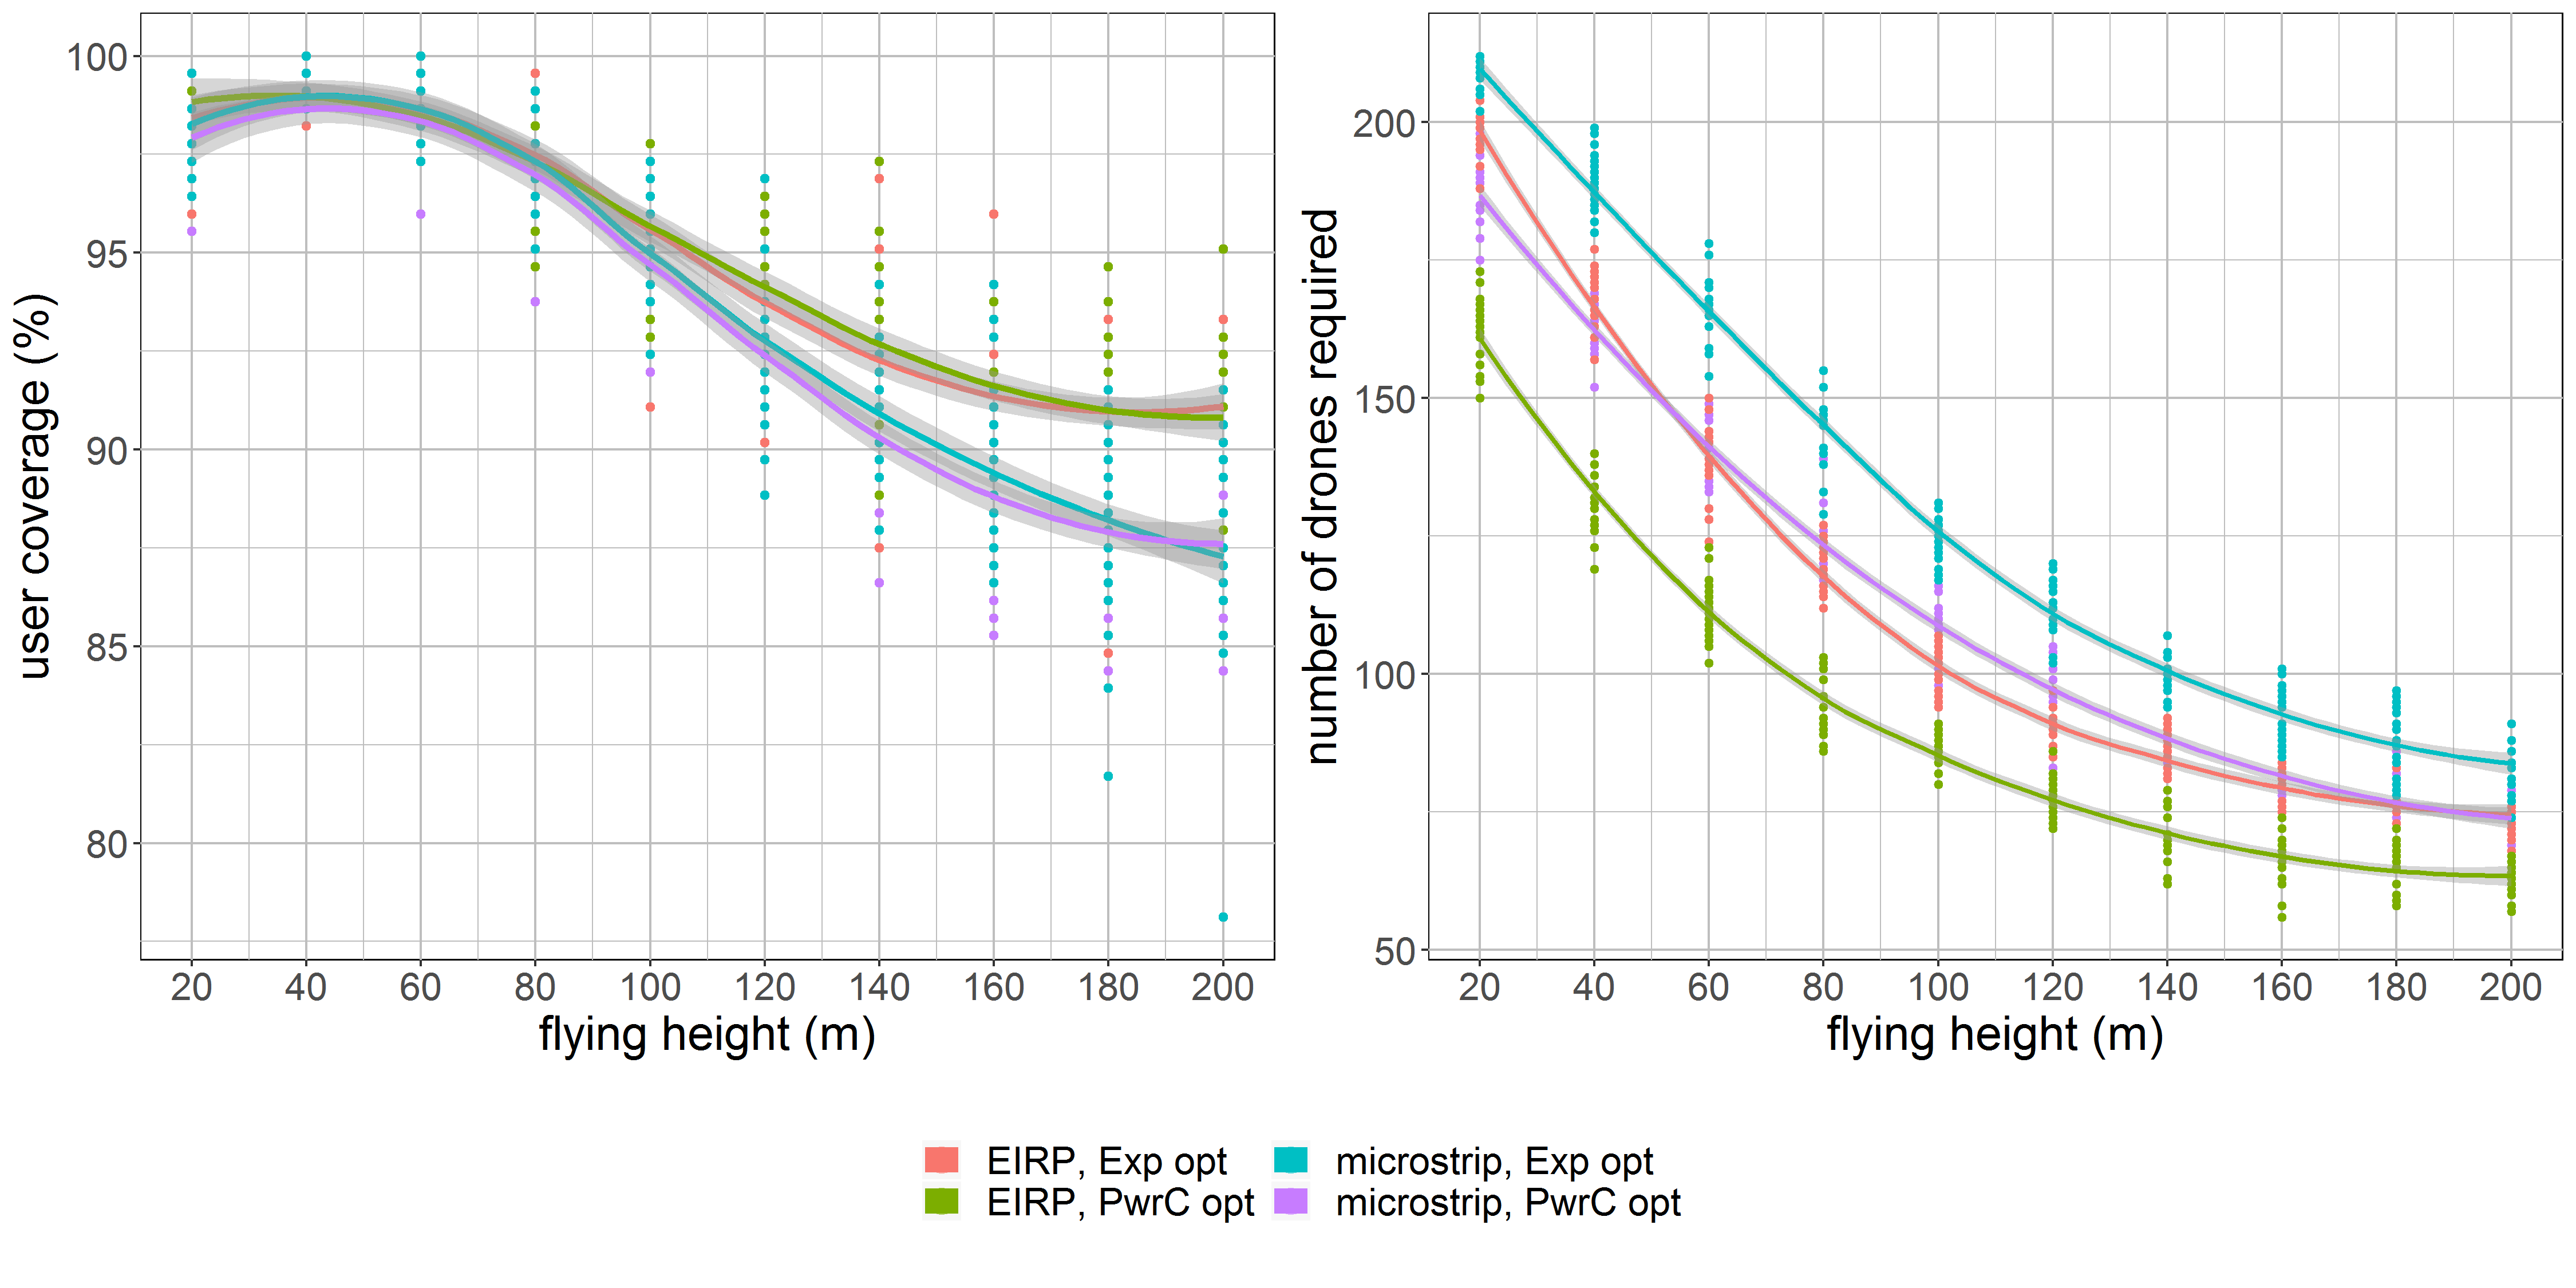
\includegraphics[width=\linewidth]{../results/s3/fhvsnumdronesAndCov.png}
  \caption{This graph shows how much \acs{UAV}s are required at different flying heights while trying to achieve a 100\% coverage.}
  \label{fig:s3a_numDronesAndCov}
\end{figure}

Figure \ref{fig:s3a_fourSourcesMatrix} shows how each source contributes to the total \gls{SAR}.
A first consequence of raising the flying altitude from 
 20 to 200 metres is the increase \gls{SAR} from the user's own device situated
 with 89 and 141 $nW/kg$; a behaviour also explained in the first scenario.
Figure \ref{fig:s3a_fourSourcesMatrix} shows that once the flying altitude surpasses the \gls{NLOS} of the buildings, 
around 70 to 80 metres, the SAR from the serving \gls{UABS} remains 
more or less constant for all configurations.
The $SAR^{myUABS}$ varies for these higher flying heights 
around $160\ nW/kg$ for microstrip \gls{PwrC Opt} networks and around $98\ nW/kg$ for microstrip \gls{Exp Opt} and \gls{EIRP} \gls{PwrC Opt} networks.
An \gls{EIRP} \gls{Exp Opt} network is situated around $47\ nW/kg$.
These higher flying altitudes will also result in an increase in electromagnetic radiation from 
other \gls{UABS}s.
Raising the flying altitude from 20 to 200 metres will increase the
the $SAR^{otherUABS}$ between 115 and 140 $nW/kg$ for \gls{EIRP} antennae and between 54 and 74 $nW/kg$ for microstrip patch antennae
for both optimization strategies.


\begin{figure}[h!]
  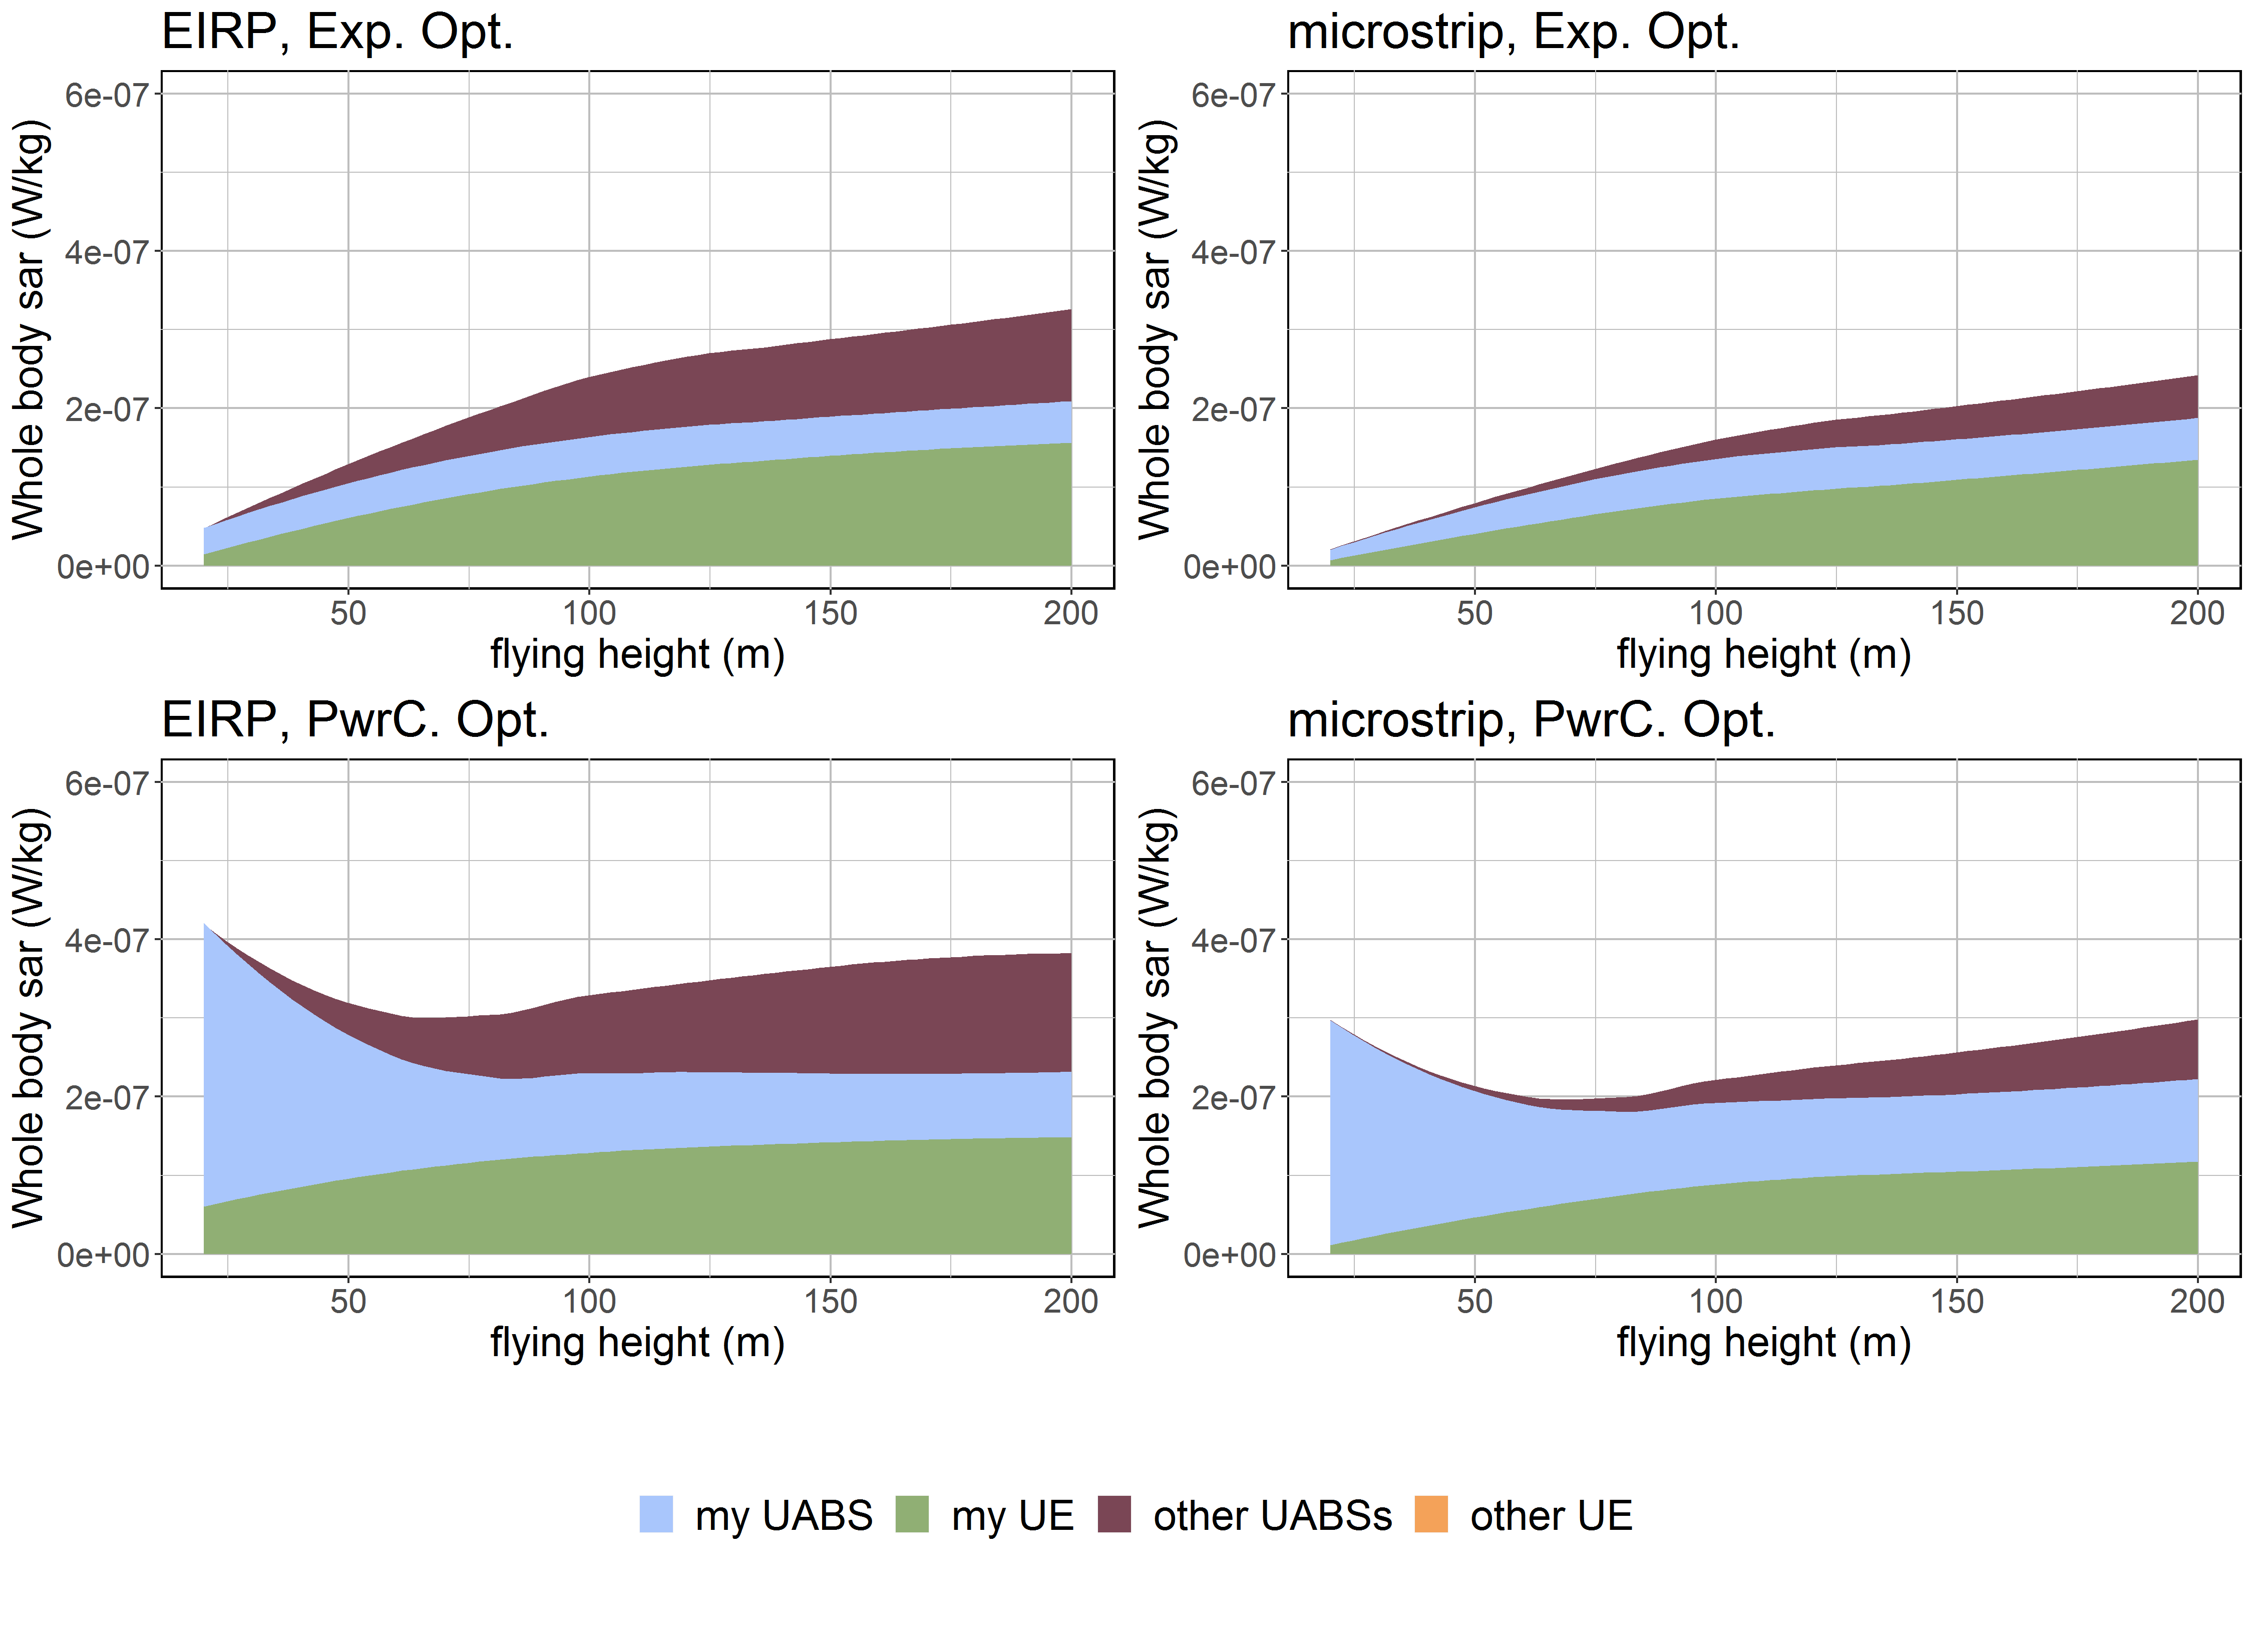
\includegraphics[width=\linewidth]{../results/s3/fhFourSources.png}
  \caption{Each chart corresponds with one of the four possible configurations. The contribution of each source towards the total 
  \gls{SAR} for a varying flying height is shown.}
  \label{fig:s3a_fourSourcesMatrix}
\end{figure}

\subsubsection{Variable Number of Users}

The second evaluated parameter of scenario III is a variable number of users while the flying height is fixed to 100 metres.  
Figure \ref{fig:s3b_numdronesAndCov}.a shows how the tool tries to reach a 100\% coverage. The percentage
of covered users is slightly less for smaller networks. For only 50 users, an average 
coverage of around 93\% is achieved while a network with 600 users has a coverage of around 97\%.
Figure \ref{fig:s3b_numdronesAndCov}.b shows how the tool requires more \gls{UAV}s for these large 
populations. 
The difference in optimization strategy is very little for a small amount of people but increases very quickly. 
When the population increases from 50 to 600 users,
 200 more \gls{UABS}s are required by a microstrip \gls{Exp Opt} network 
 around 130 more \gls{UABS}s for an \gls{EIRP} \gls{Exp Opt} network or a microstrip \gls{PwrC Opt} network
 and 110 more \gls{UABS}s for an \gls{EIRP} \gls{PwrC Opt} network.
This is an expected behaviour  when looking at scenario II where, with only one \gls{UABS} available, 
the percentage of covered users decreases for these larger populations.

\begin{figure}[h]
  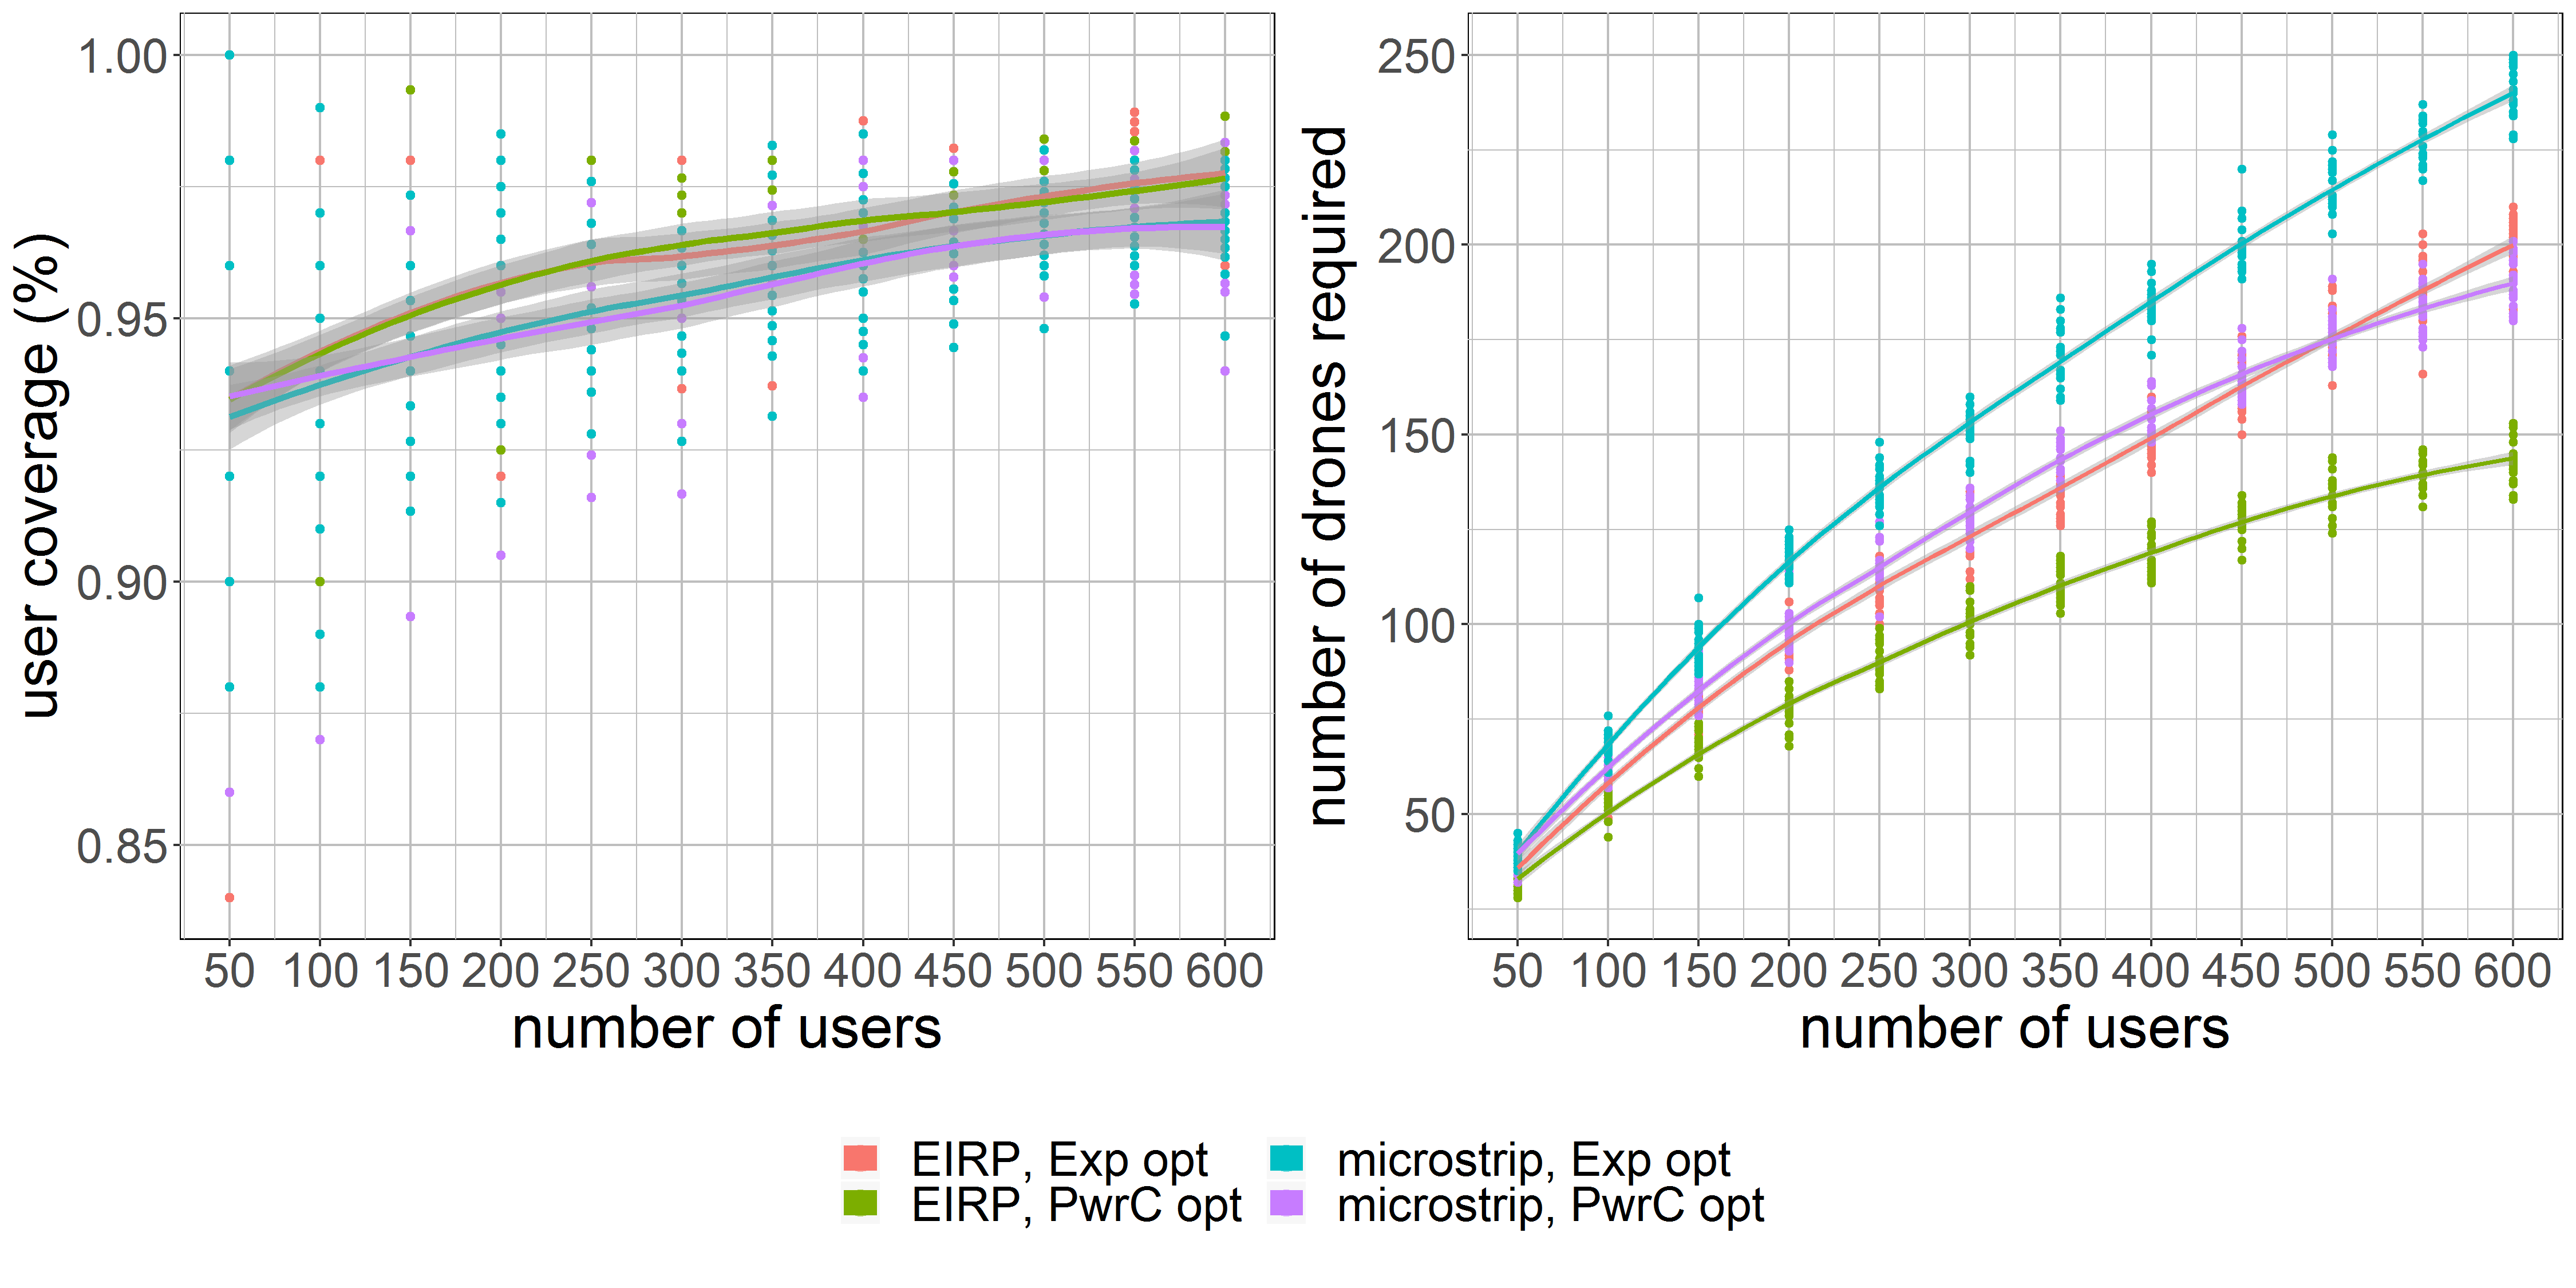
\includegraphics[width=\linewidth]{../results/s3/uvsnumdronesAndCov.png}
  \caption{This graph shows how much \acs{UAV}s are required for different flying heights while trying to achieve a 100\% coverage.}
  \label{fig:s3b_numdronesAndCov}
\end{figure}


Figure \ref{fig:s3b_dlAndPC} shows that the electromagnetic radiation and power consumption increase for larger 
populations which is normal since more drones will be available.
When the population increases from 50 to 600 users, the electromagnetic radiation increases 
between 80 and 130 $mV/m$ depending on the configuration. The power consumption with 50 users is for all configurations around 
20 $W$. Once the population is increased to 600 users, a microstrip \gls{Exp Opt} network will require 130 $W$, 
 a microstrip \gls{PwrC Opt} network requires 117 $W$,
\gls{EIRP} \gls{Exp Opt} networks require 107 $W$ and \gls{EIRP} \gls{PwrC Opt} network requires 92 $W$.

The correct behaviour of the decision algorithm became already clear in the previous subsection \ref{S3A} but is also
confirmed here. 
When comparing both optimization strategies, a power consumption optimized network requires around 5 $W$ less but exposes its users between 27 $mV/m$ and 30 $mV/m$ more than
exposure optimized networks. 
Further, it is also noticed that \gls{isotropicradiator}s cause more electromagnetic radiation for less energy
compared to microstrip patch antennae. 
When comparing the two types of antennae for a default number of 224 users, 
an \gls{isotropicradiator} will expose the average user 
between 25 $mV/m$ and 27 $mV/m$ more while requiring around 12 $W$ less than when the network would be using a microstrip patch antennae.


\begin{figure}[h!]
  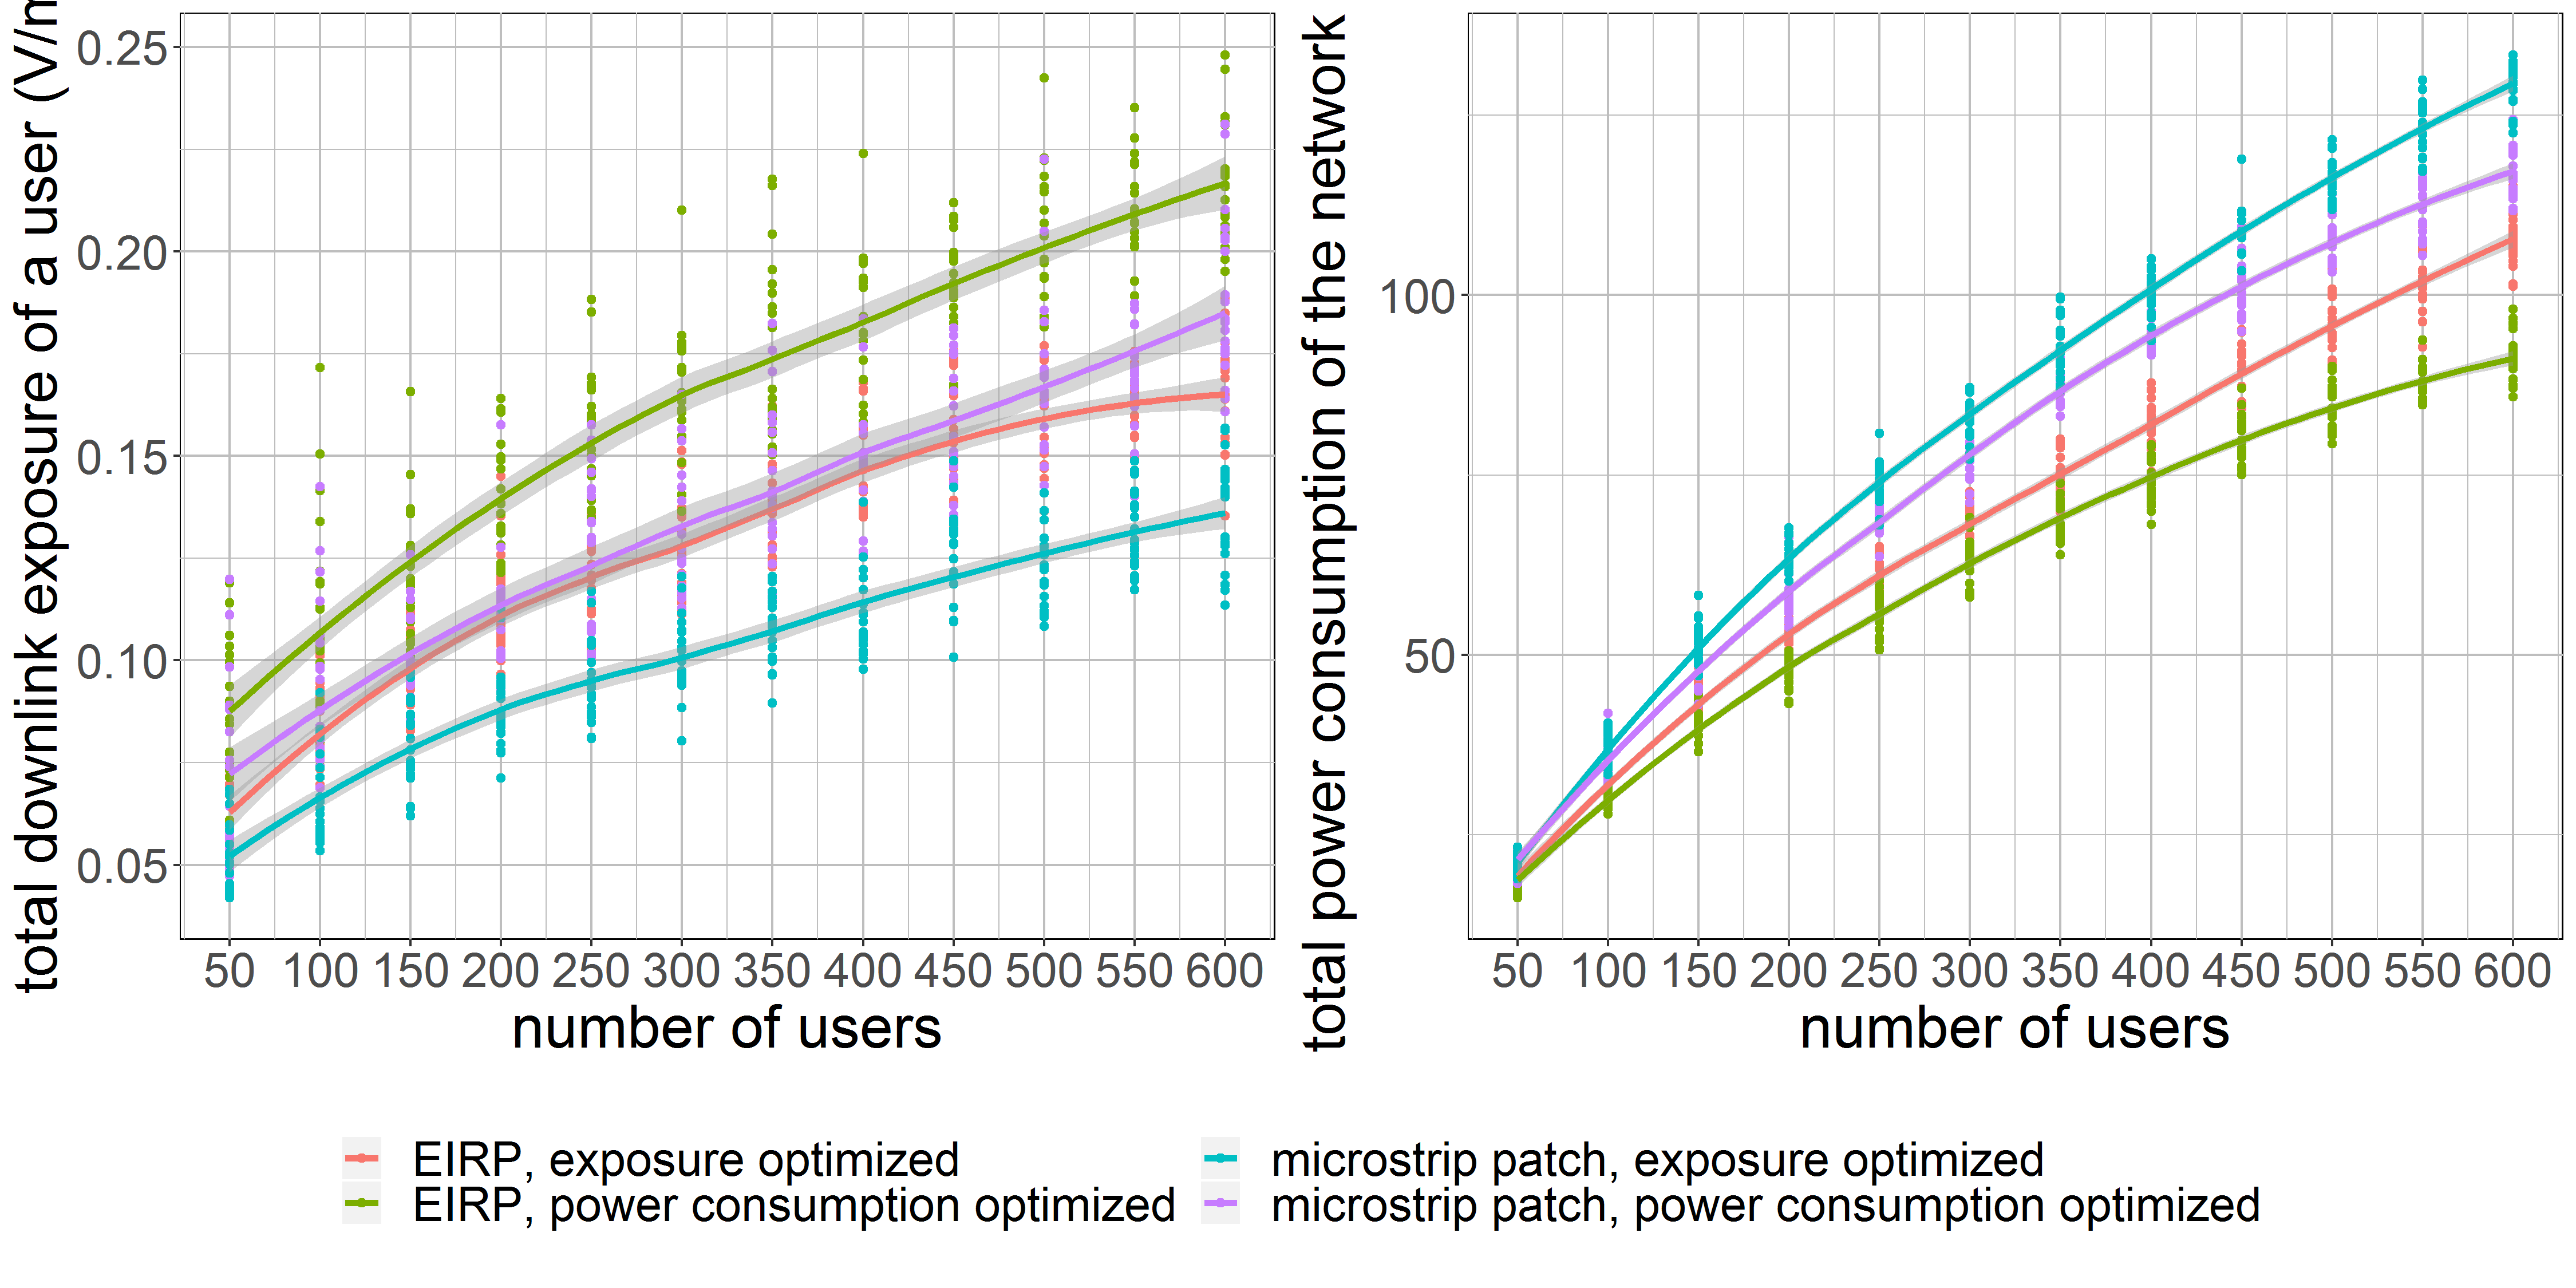
\includegraphics[width=\linewidth]{../results/s3/uvsdlAndPc.png}
  \caption{The influence of the population size on the downlink electromagnetic radiation (a) and power consumption (b).}
  \label{fig:s3b_dlAndPC}
%\bigbreak
 % 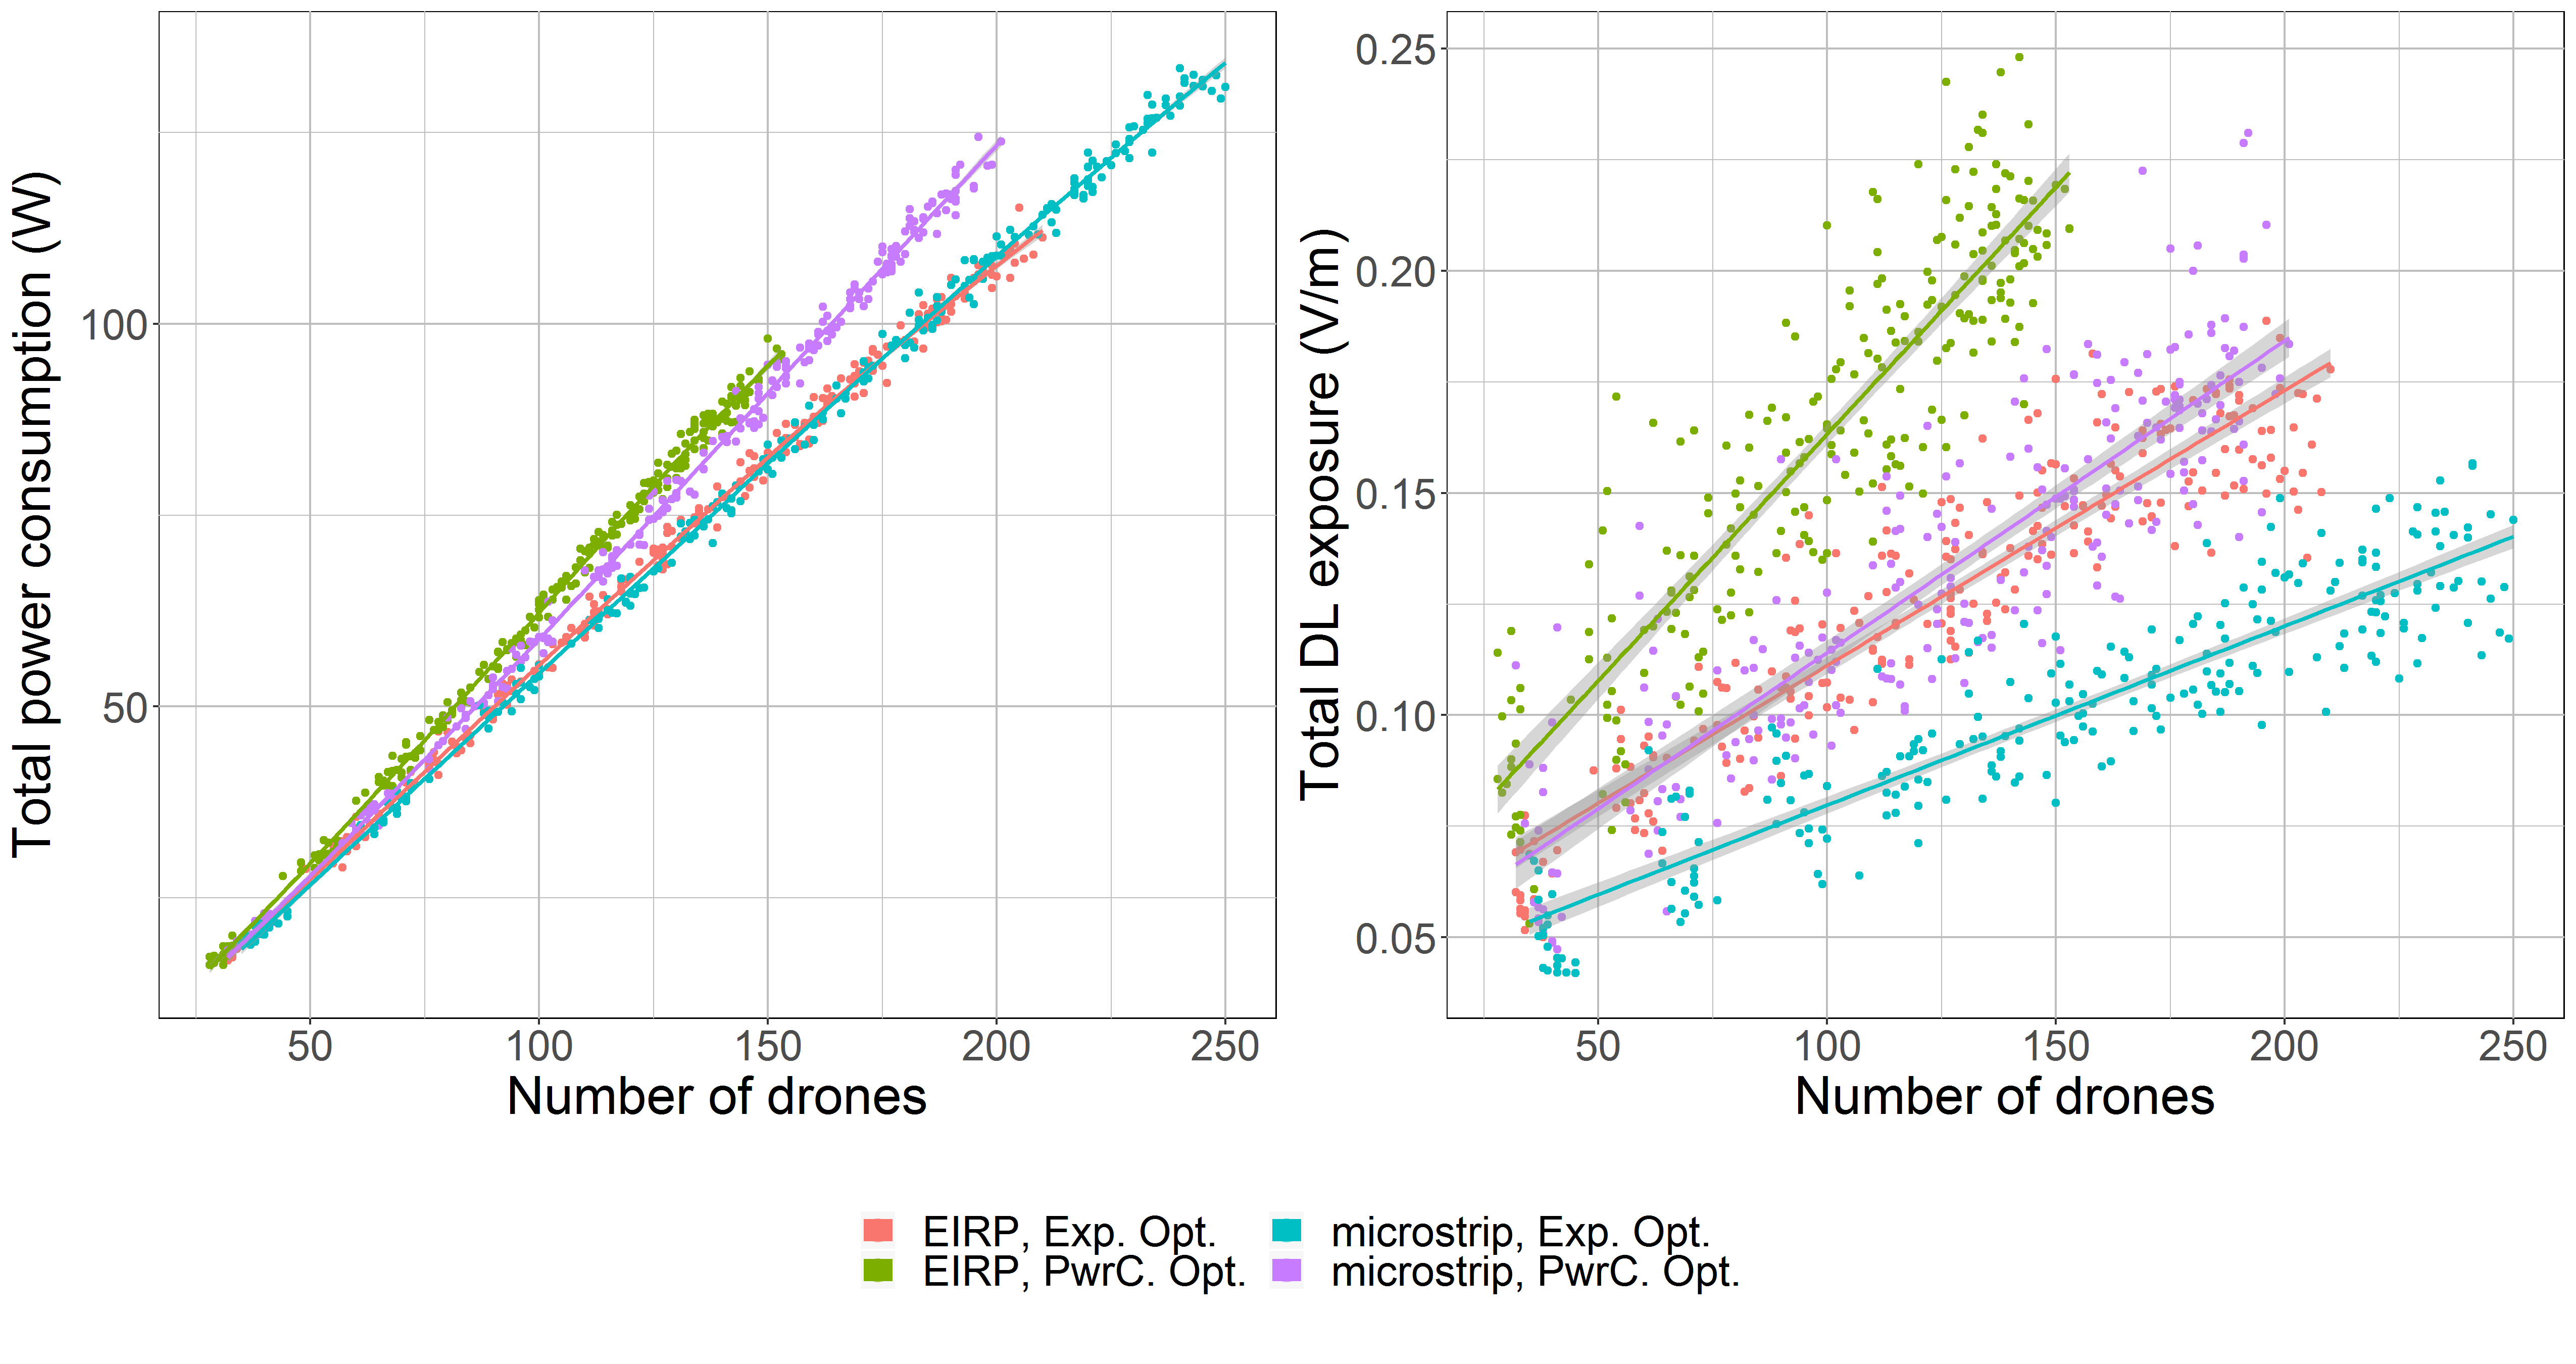
\includegraphics[width=\linewidth]{../results/s3/u_numdronesvsdlAndPc.png}
  %\caption{The influence of the number of UABSs on the downlink electromagnetic radiation (a) and power consumption (b).}
  %\label{fig:s3b_dlAndPC2}
\end{figure}

\begin{figure}[h!]
  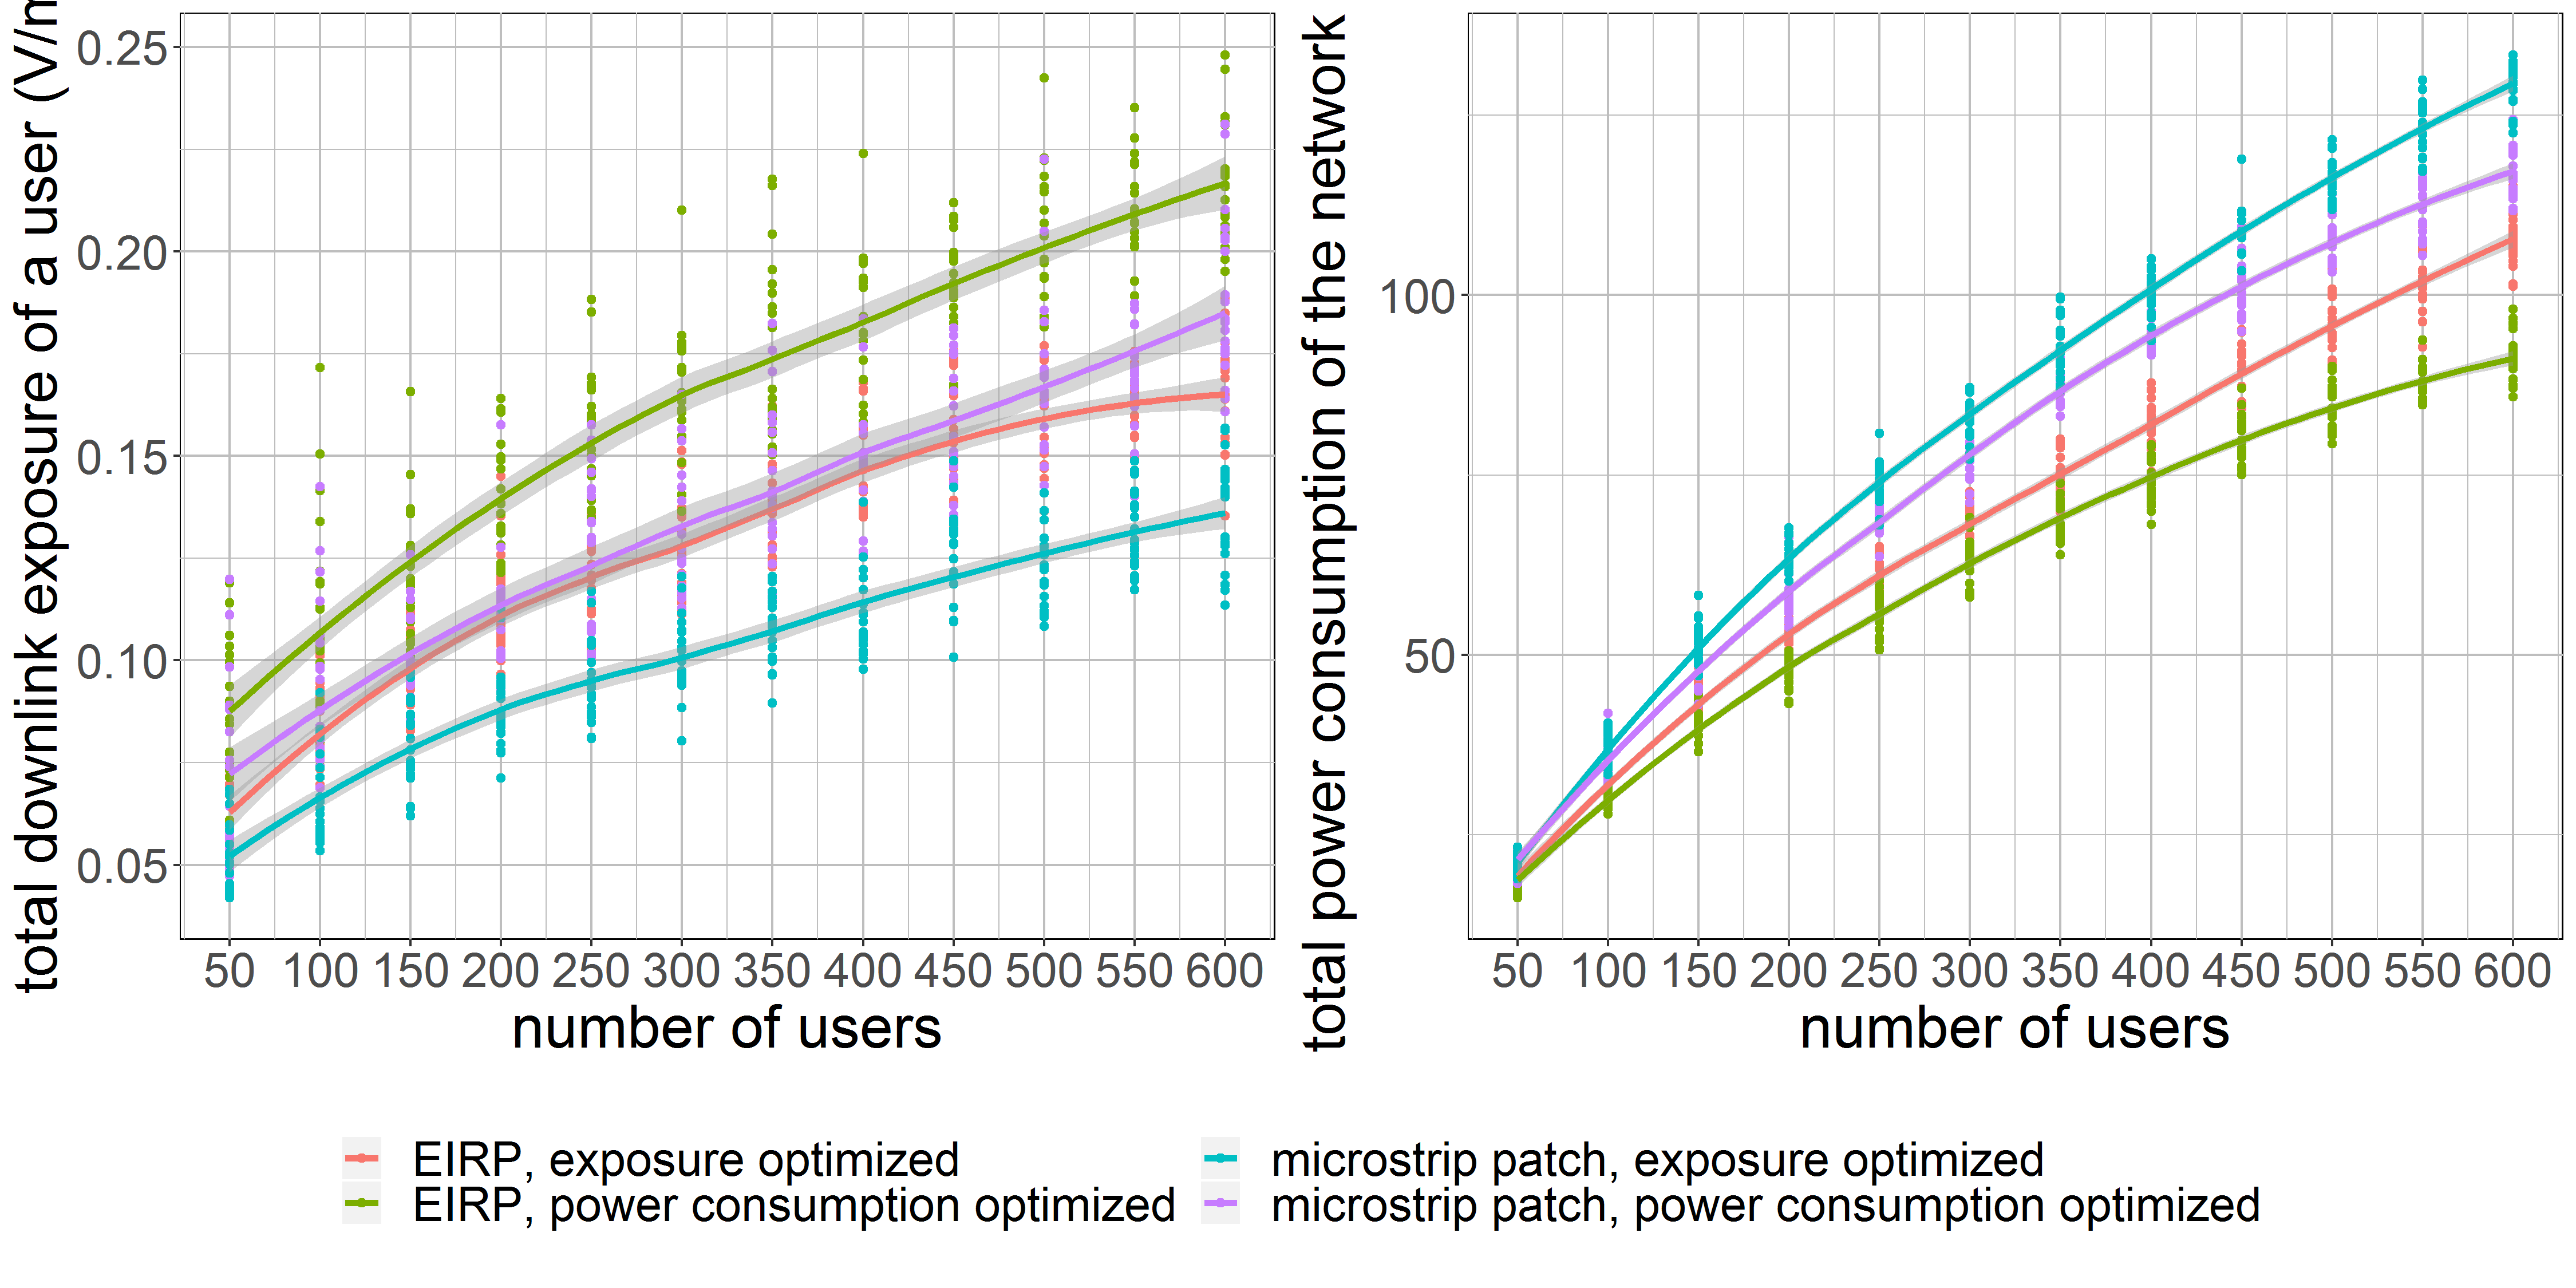
\includegraphics[width=\linewidth]{../results/s3/uvsdlAndPc.png}
  \caption{These two figures show how the number of users influences the downlink electromagnetic radiation of the average user (left) and 
  power consumption of the entire network (right) for an unlimited number of drones.}
  \label{fig:s3b_dlAndPC}
\end{figure}

Figure \ref{fig:s3b_fourSourcesMatrix} represents the 
\gls{SAR} from the weighted average user and shows how the \gls{SAR} coming from the user's own device remains almost constant. 
The flying altitude is always the same so 
also the required energy to cover that distance will remain the same. 
For both optimization strategies, the $SAR^{myUE}$ for networks with \gls{isotropicradiator}s vary around $1.1\ \mu W/kg$  %between 1 $\mu W/kg$ and 1.2 $\mu W/kg$ 
 and around  0.7 $\mu W/kg$ for networks using microstrip patch antennae.
The $SAR^{myUABS}$ barely increases in an exposure optimized network and is situated around 0.5 $\mu W/kg$ for both antennae.
The power consumption optimized network also starts around 0.5 $\mu W/kg$ but increases when more users become online. 
A normal behaviour when considering that these \gls{UABS}s try to cover much more users. Therefore, the $SAR^{myUABS}$ 
with 600 users increases up to 1 $\mu W/kg$ for an \gls{isotropicradiator} and almost 2 $\mu W/kg$ for a microstrip patch antenna.
The \gls{SAR} value that increases the most is $SAR^{otherUABS}$ which 
starts really low with less than 0.1 $\mu W/kg$ for 50 users for all configurations. 
The \gls{SAR} increases however very fast. The biggest increase is noticed in an \gls{EIRP} \gls{PwrC Opt} network 
where 3 $\mu W/kg$ is measured for 600 users. The $SAR^{otherUE}$ increases the least for microstrip \gls{Exp Opt} with 
only 1 $\mu W/kg$ for 600 users.
\begin{figure}[h!]
  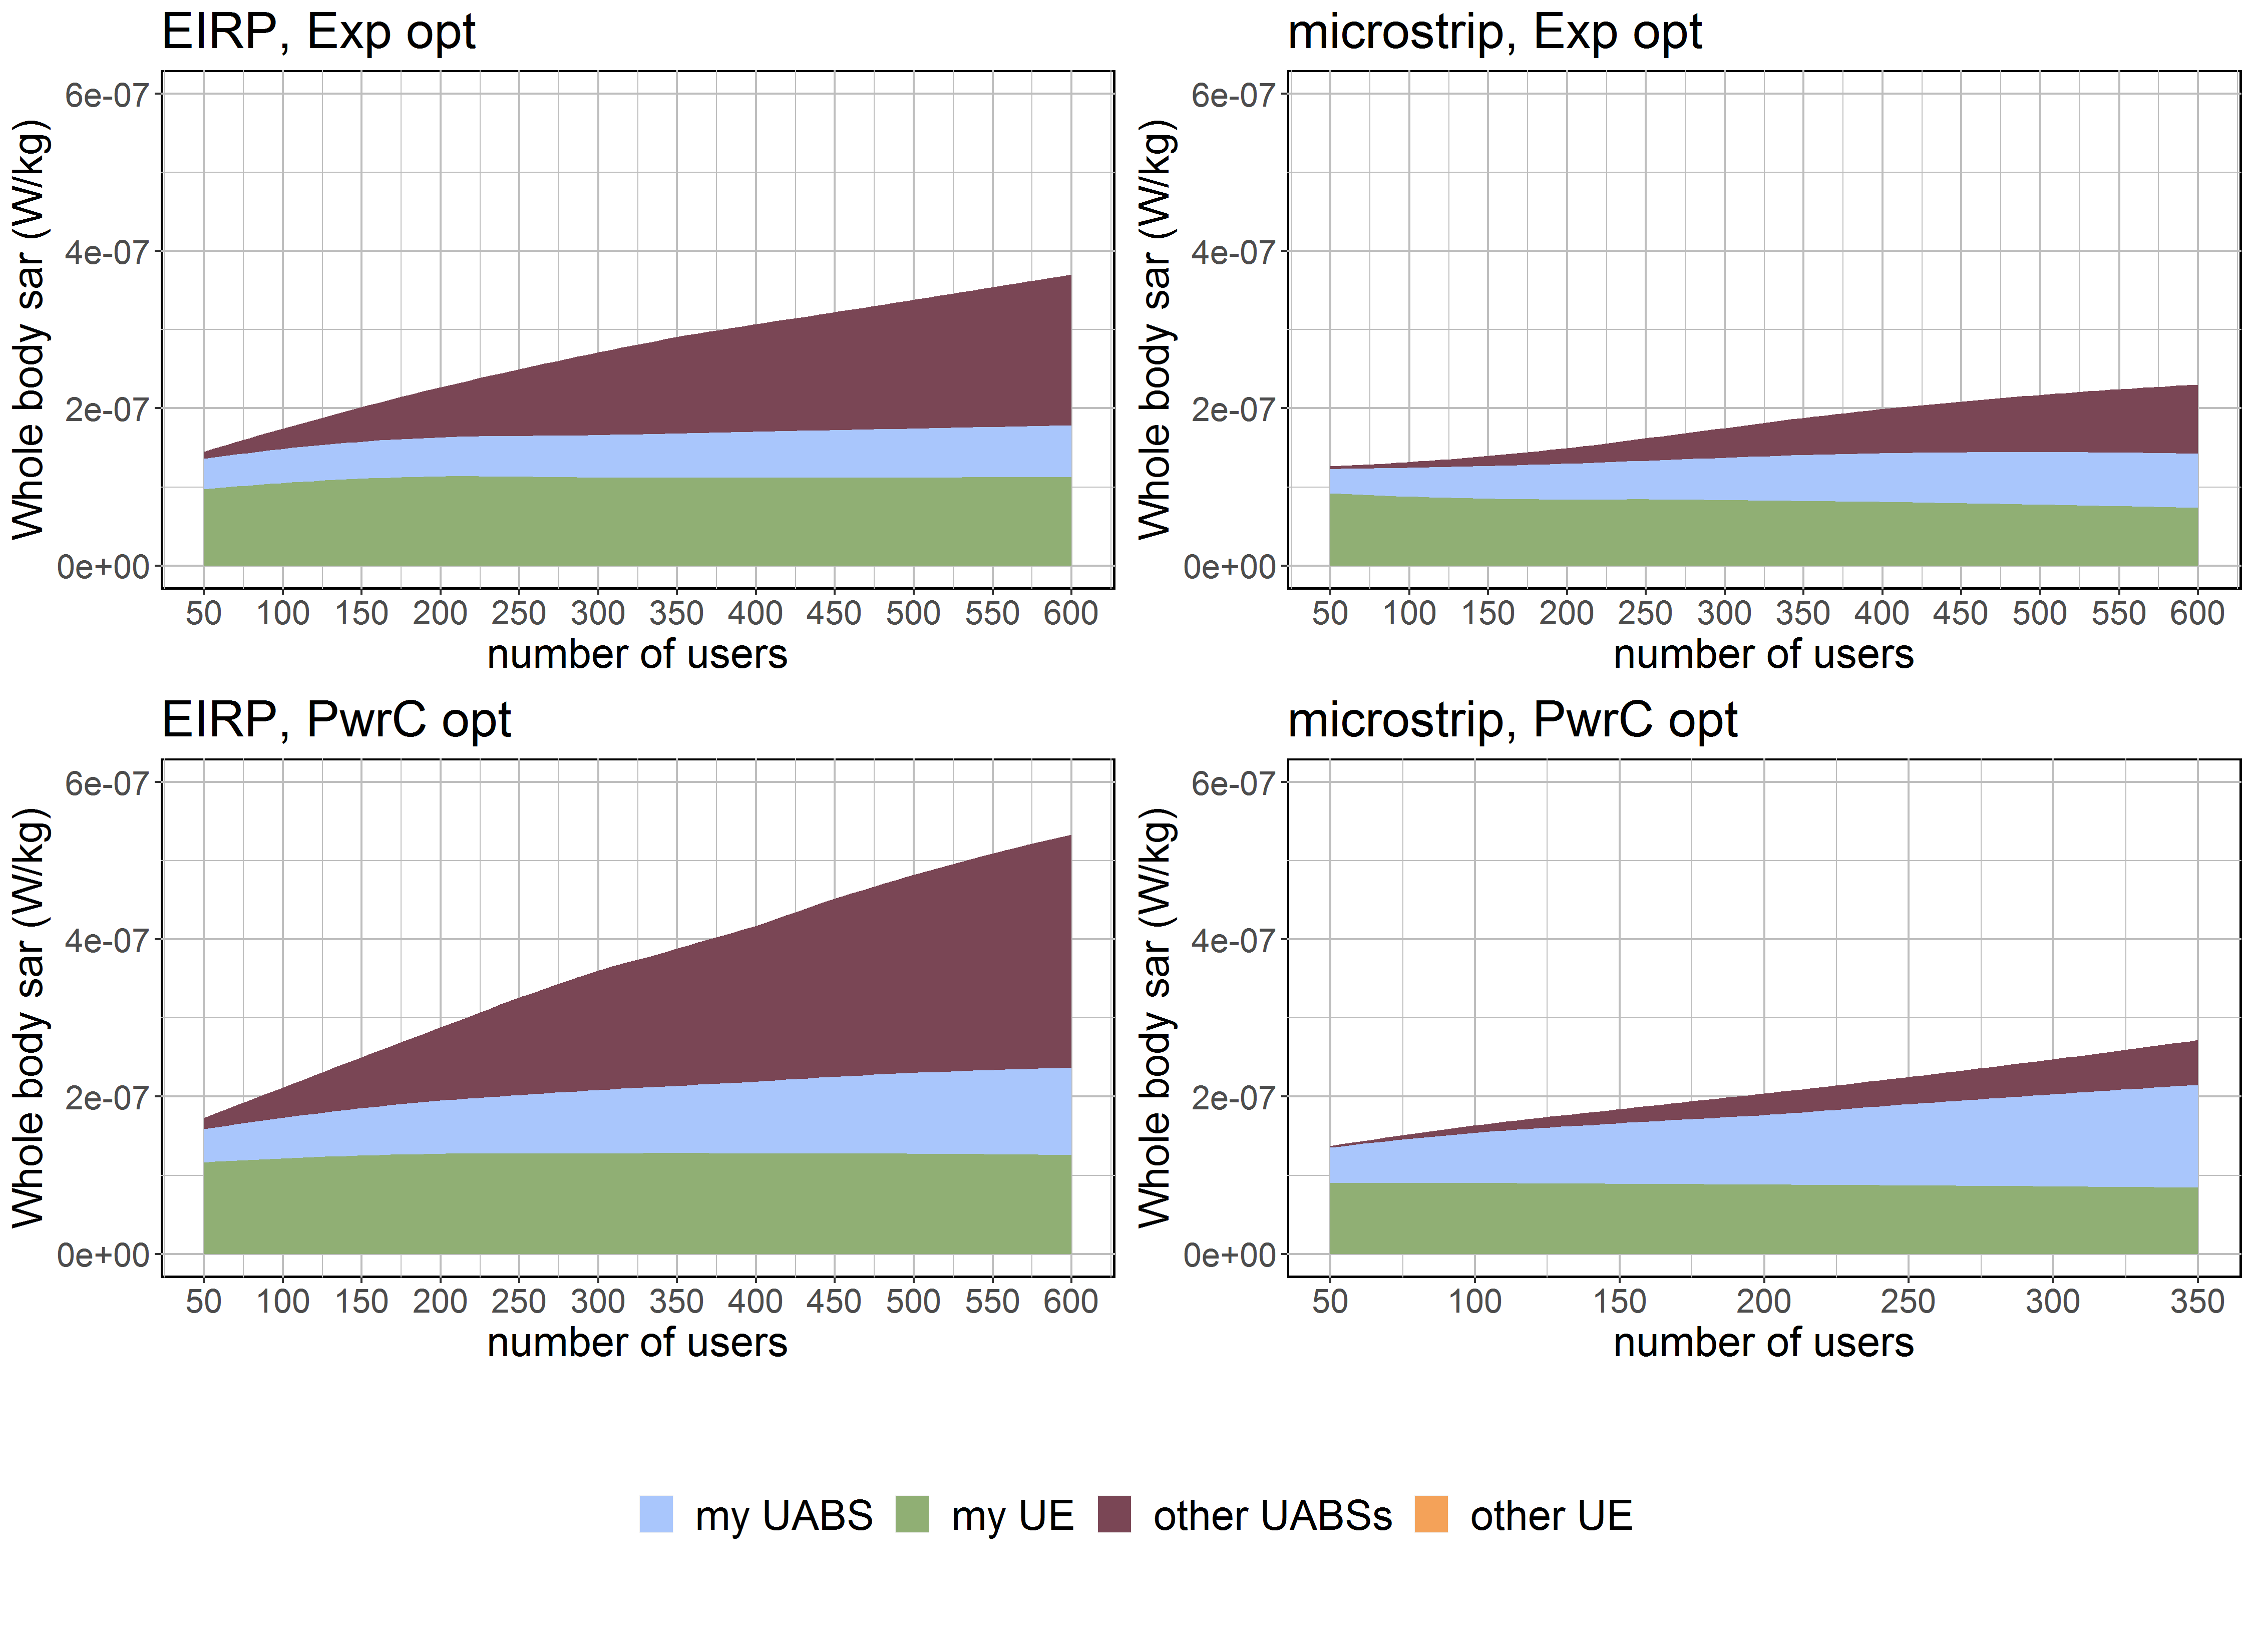
\includegraphics[width=\linewidth]{../results/s3/uFourSources.png}
  \caption{Each figure corresponds with a certain configuration and shows how the \acs{SAR} 
  from different sources are influenced by an increasing population density. An unlimited number of \acs{UABS}s is available.
}
  \label{fig:s3b_fourSourcesMatrix}
\end{figure}

\section{Conclusion}
%How can a UABS network be optimized to minimize global exposure or overall power consumption? 
Literature showed that a network can be optimized towards either the power consumption of the entire network 
or the electromagnetic exposure of the average user using a fitness function \cite{J1}.
However, the fitness function should be used with care considering that \gls{UABS}s can be placed anywhere as opposed to 
the transmission towers from \cite{J1} who have a predetermined position. 
In an \gls{Exp Opt} network, this causes a lot of users to get a \gls{UABS} all by 
themselves because this is the best approach to minimize exposure.
A \gls{PwrC Opt} network on the other hand will try to limit the number of drones 
in order to save energy. 
So as a rule of thumb: an \gls{Exp Opt} network will result in a lot of low powered devices (increasing the overall power consumption)
while a \gls{PwrC Opt} network results in a few high powered devices (increasing the exposure of the average user).
If the goal is to remain in the air for a longer period of time, an \gls{Exp Opt} network is recommended because the power consumption of 
an individual \gls{UABS} is lower.
On the other hand, a \gls{PwrC Opt} network is cheaper because less drones are involved. 
Moreover, the results show that the electromagnetic radiation in a \gls{PwrC Opt} network (with high powered \gls{UABS}s)
is far below the thresholds enforced by the Flemish government.

The user's main sources of exposure are the user's own device and the \gls{UABS} who is serving him, followed by all
other \gls{UABS}s in the network. 
When the population increases, there is not only more radiation from \gls{UE} but also 
from more \gls{UABS}s that are serving the other users.
The exposure from other people's \gls{UE} is so low that it can be neglected.
An \gls{Exp Opt} network will limit the total exposure mainly by trying to reduce the exposure from other \gls{UABS}s.

%1)	How does the network behave differently after the introduction of a realistic antenna?
A directional microstrip patch antenna is introduced because it gives several advantages compared to omnidirectional antennae.
Directional antennae are able to focus their energy there where it is needed, namely towards the ground. Microstrip patch antennae 
further benefit from their thin and lightweight design. The performance 
of this directional microstrip patch antenna has been compared to a 
fictional \gls{isotropicradiator}.
This \gls{isotropicradiator} has higher exposure and coverage for less power, compared to realistic antennae like microstrip patch antennae
because of the absence of attenuation, and can hypothetically be compared with an antenna with a very big aperture angle.
This type of antenna can achieve the same coverage with less
resources like power and number of drones. 
A microstrip patch antenna with a more limited aperture angle of \ang{90} requires more resources but 
causes less sideways radiation. So the exposure from other \gls{UABS}s will be way less.

\begin{figure}[h!]
  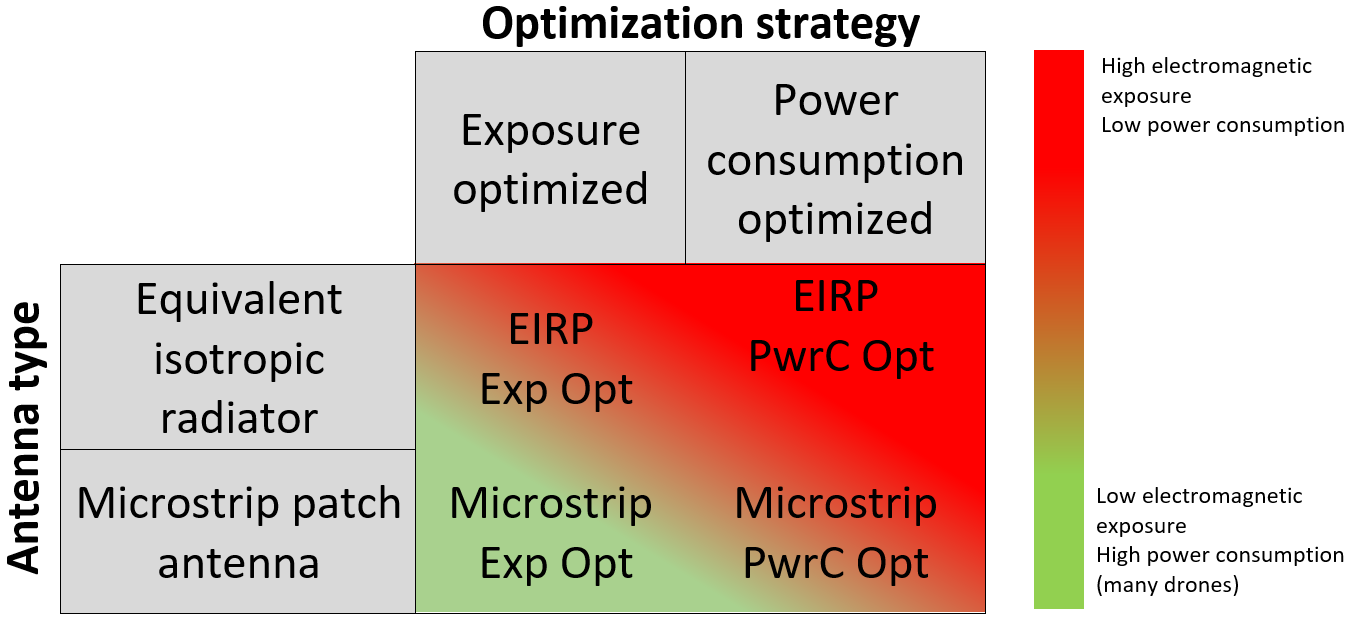
\includegraphics[width=\linewidth]{fourCasesMatrixSol.png}
  \caption{Matrix with the four possible configurations, colour-coded based on the results.}
  \label{fig:resultIllustration}
\end{figure}

Remarkable is that an \gls{EIRP} \gls{Exp Opt} network behaves very similar to a microstrip \gls{PwrC Opt} network as shown 
in figure \ref{fig:resultIllustration}.
This results in the best of both worlds. 
The microstrip patch antenna will generate less electromagnetic radiation by design and
 the power consumption optimization reduces the number of required drones and power. A microstrip patch antenna with an aperture 
 angle of \ang{90} is considered as a good solution but if budget is limited, an antenna with a larger aperture angle 
 would further reduce cost without interfering with the Flemish legislation regarding electromagnetic exposure.

The electromagnetic radiation of an \gls{Exp Opt} network increases with higher flying altitudes.
Around 80 metres, the exposure from the  user's device surpasses the exposure from the serving \gls{UABS}.
On the other hand, a \gls{PwrC Opt} network shows that the lowest exposure is measured around 70 to 80 metres.
Further, the results also show that the number of required drones decreases when the flying height becomes larger; a conclusion that was also made in \cite{J2}.
When also considering the results from \cite{U1} where a flying altitude from 
80 metres is suggested for an optimal access and backhaul connectivity, a flying height 
of 80 metres is also here proposed for the city centre of Ghent.

In short, a \gls{PwrC Opt} network is proposed with a fixed flying height of 80 metres. A microstrip patch 
antenna with a sufficiently large aperture angle is a good starting point. However, different antenna configurations should 
be investigated.

\section*{Acknowledgement}
Special thanks to the WAVES research group at Ghent University for providing 
access to their capacity based deployment tool and therefore making this research possible.

\bibliographystyle{ieeetr}
\bibliography{referenties}


\end{document}
